%
% Chapter 6
%

\chapter{Event Selection}
\label{evt_sel}

\section{Introduction}
\label{evt_sel_intro}
This chapter summarizes the event selection criteria for the analysis. The signal topology consists of an isolated lepton, \Pgm\, or \Pe, along with an oppositely charged isolated tau lepton (\taum, \taue, or \tauh). Jets misidentified as electrons or muons are suppressed by imposing isolation requirements. The events are first categorized into \mutau and \etau and then further divided into leptonic and hadronic channels based on tau decay mode. Figure ~\ref{fig:feynman} shows the corresponding Feynman diagrams for the LFV \Hmt and \Het decays.

\begin{figure}[htbp]
  \centering
  \subfigure[]{ 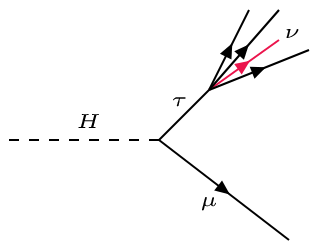
\includegraphics[width=0.3\textwidth]{plots/chapter6/Feynman/Hmuhad.png} }
  \subfigure[]{ 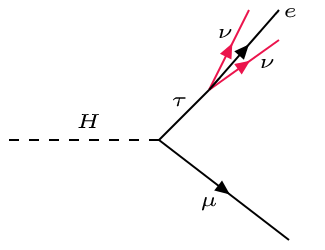
\includegraphics[width=0.3\textwidth]{plots/chapter6/Feynman/Hmue.png} } \\
  \subfigure[]{ 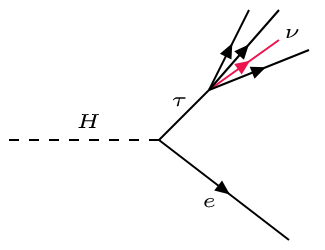
\includegraphics[width=0.3\textwidth]{plots/chapter6/Feynman/Hehad.png} }
  \subfigure[]{ 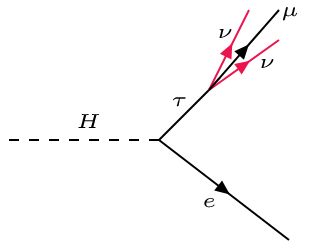
\includegraphics[width=0.3\textwidth]{plots/chapter6/Feynman/Hemu.png} } \\
  \caption{Feynman diagrams of lepton-flavor violating Higgs-boson decays. The first row shows diagrams for the Higgs boson coupling to \mutau (a,b). Couplings to \etau (c,d) are shown in the second row. Taus can decay leptonically or hadronically. Feynman diagrams are shown for the leptonic decay of taus (b,d) and the hadronic decay of taus (a,c).}
  \label{fig:feynman}
\end{figure}

The final states of this analysis are similar to the \Htt decay allowed by the SM and since been observed ~\cite{Sirunyan:2017khh}. However, there are some significant kinematic differences. The LFV \Hmuhad and \Hmue (\Hehad and \Hemu) decays consist of a muon (an electron) that comes directly from the Higgs and has a hard \pt spectrum, along with a hadronically decaying tau or a softer electron (muon) that comes from the tau lepton of opposite sign charge, and missing transverse momentum from the tau decay. Also, there are fewer neutrinos in LFV decays, coming from the decay of the single \Pgt. The decay products of this highly boosted tau are closely aligned, leading to a narrow separation between the visible decay products of the tau and the \ptvecmiss in the azimuthal plane. The same is not true in the \Htt decays. These differences are illustrated pictorially in Figures ~\ref{fig:htt_v_lfv_mt} and ~\ref{fig:htt_v_lfv_et}.

\begin{figure}[htbp]
  \centering
  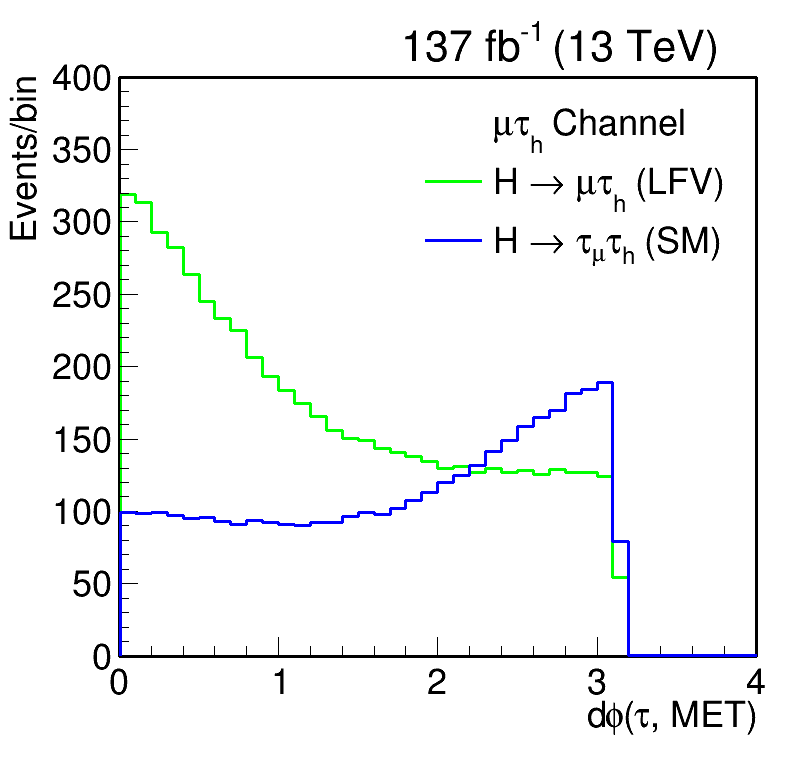
\includegraphics[width=0.45\textwidth]{plots/chapter6/LFVvSM/MTdphi.png}
  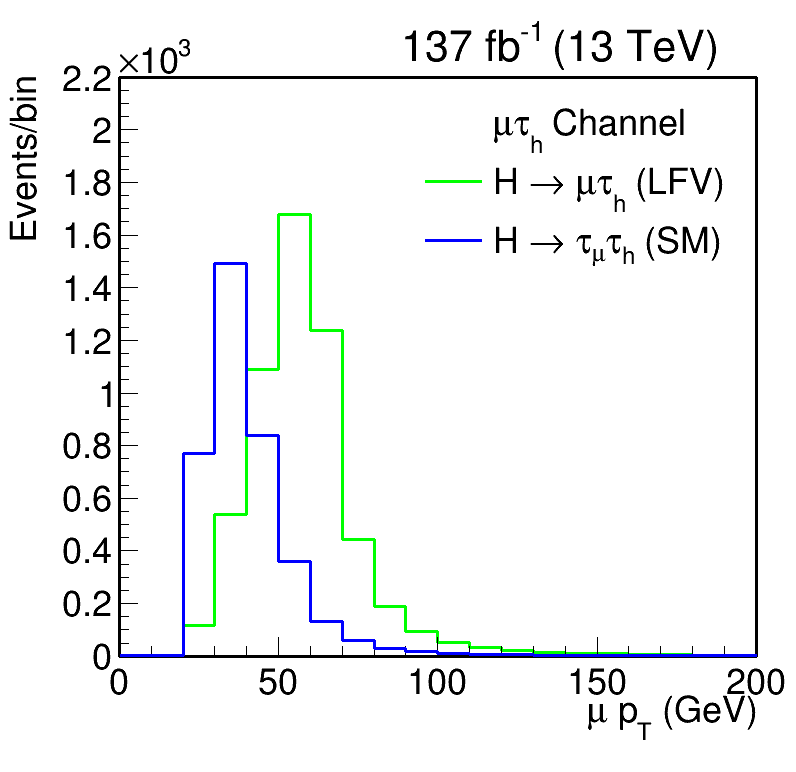
\includegraphics[width=0.45\textwidth]{plots/chapter6/LFVvSM/MTmpt.png} \\
  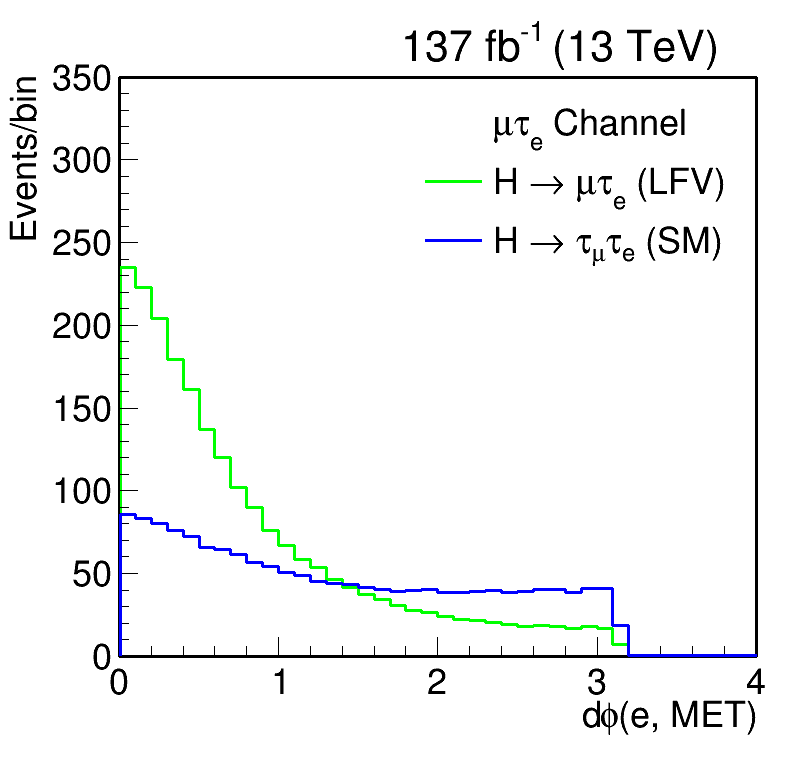
\includegraphics[width=0.45\textwidth]{plots/chapter6/LFVvSM/MEdphi.png}
  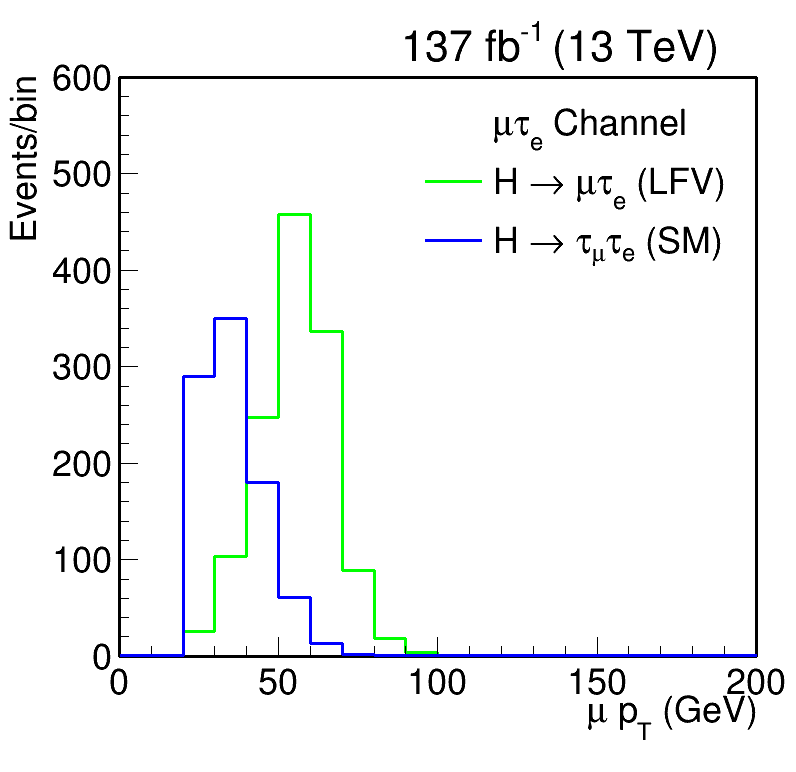
\includegraphics[width=0.45\textwidth]{plots/chapter6/LFVvSM/MEmpt.png} \\
  \caption{Illustration of the differences in $d\phi(\ell = \Pgt \; or \; \Pe, MET)$ and $\pt^{\Pgm}$ spectrums in LFV and SM \Htt processes.}
  \label{fig:htt_v_lfv_mt}
\end{figure}

\begin{figure}[htbp]
  \centering
  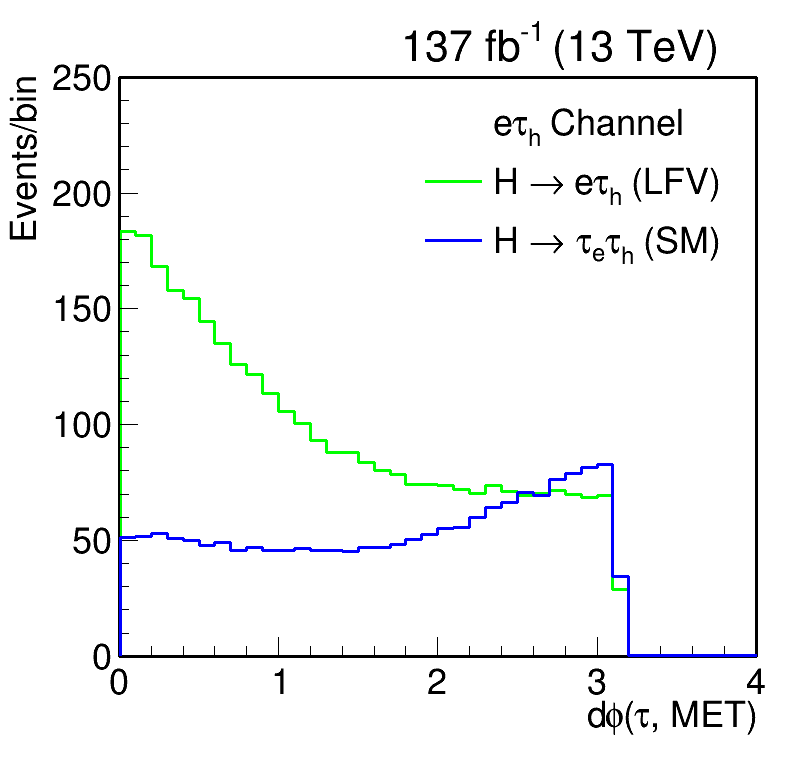
\includegraphics[width=0.45\textwidth]{plots/chapter6/LFVvSM/ETdphi.png}
  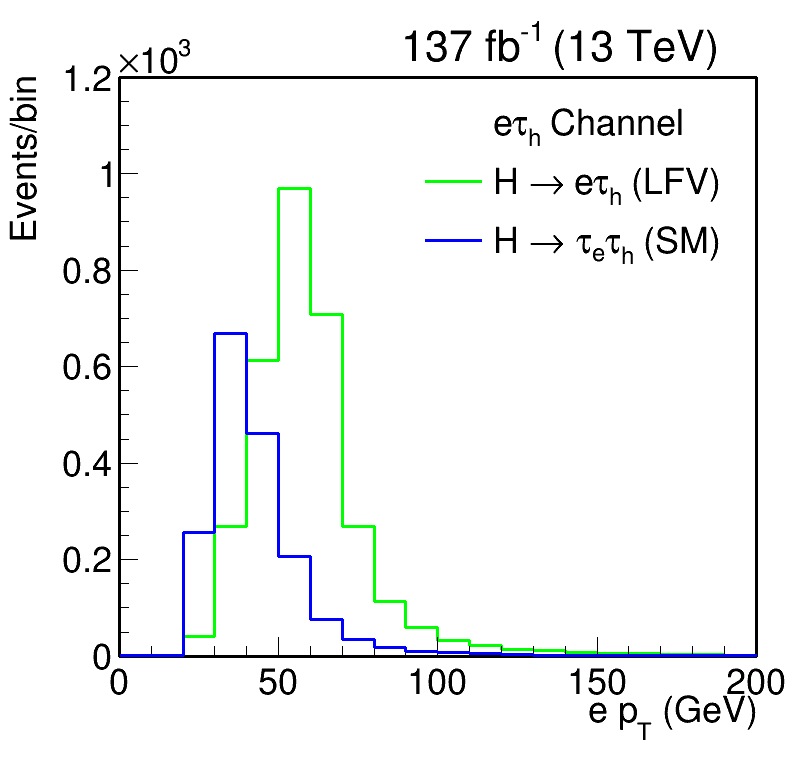
\includegraphics[width=0.45\textwidth]{plots/chapter6/LFVvSM/ETept.png} \\
  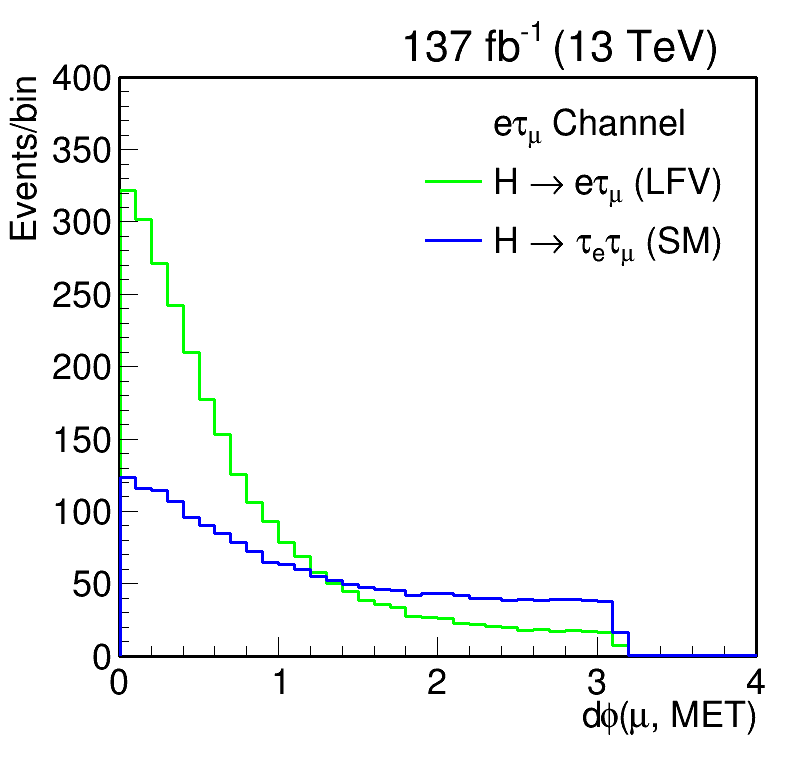
\includegraphics[width=0.45\textwidth]{plots/chapter6/LFVvSM/EMdphi.png}
  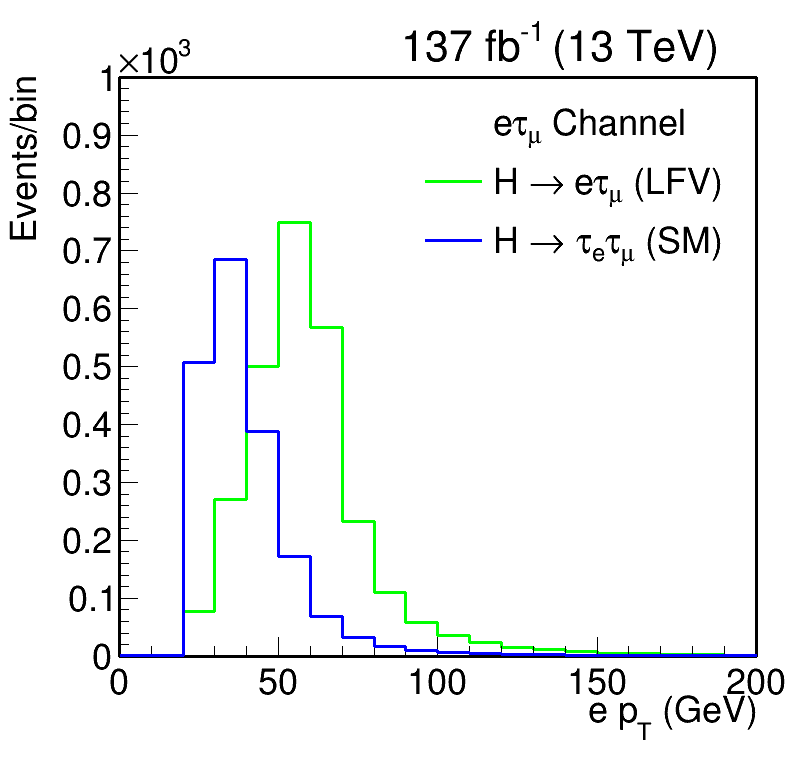
\includegraphics[width=0.45\textwidth]{plots/chapter6/LFVvSM/EMept.png} \\
  \caption{Illustration of the differences in $d\phi(\ell = \Pgt \; or \; \Pgm, MET)$ and $\pt^{\Pe}$ spectrums in LFV and SM \Htt processes.}
  \label{fig:htt_v_lfv_et}
\end{figure}

In each decay mode (\Hemu, \Hehad, \Hmue, \Hmuhad), a set of loose selection (preselection) for the respective signature is first defined. The jets in the event are required to have a $\pt > 30\GeV$ and $\abs{\eta} < 4.7$. The event in each decay channel is divided into categories based on the number of jets in the event (0-jet, 1-jet, 2-jet) to enhance the contribution of different Higgs boson production mechanisms.

The 0-jet category enhances the Gluon Gluon Fusion (GGF) Higgs production contribution, while the 1-jet category enhances the GGF Higgs production with initial-state radiation. The 2-jet category is further broken into two based on the invariant mass of the two jets (\mjj). The threshold of 550 (500)\GeV on \mjj for \mutau(\etau) channels has been optimized to give the best-expected exclusion limits. Events with $\mjj < 550(500)\GeV$ enhances GGF Higgs production contribution while $\mjj \ge 550(500)\GeV$ enhances VBF Higgs production contribution.

To better discriminate between signal and background events, a Boosted Decision Trees (BDT) discriminator is trained using simulated events, using the TMVA tool of the ROOT analysis package ~\cite{Hocker:2007ht}. After applying preselection, a binned likelihood is used to fit the distribution of a BDT discriminator for the signal and the background contributions, and we call this the BDT fit method. The collinear mass (\mcol) and the transverse mass ($\mt(\ell)$) that are used as input variables to the BDT are defined in the following paragraphs. A brief description of the BDT is given in the next section.

The \mcol provides an estimate of \mh using the observed decay products of the Higgs boson candidate. It is reconstructed using the collinear approximation based on the observation that, since $\mh \gg m_\Pgt$, the \Pgt\, lepton decay products are highly Lorentz boosted in the direction of the \Pgt\, candidate ~\cite{Ellis:1987xu}. The momentum of the neutrino coming from \Pgt\, decay can be approximated to have the same direction as the visible decay products of the \Pgt(\vectvis). Figure ~\ref{fig:METproj} shows the corresponding Feynman diagram for the \met projected in the direction of the visible decay products of tau.

\begin{figure}[htbp]
  \centering
  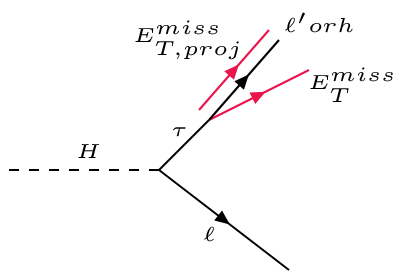
\includegraphics[width=0.49\textwidth]{plots/chapter6/Feynman/METproj.png}
  \caption{Estimation of the neutrino momentum \metproj by using the component of the missing transverse energy \met which is collinear to the visible decay products of tau in the transverse plane.}
  \label{fig:METproj}
\end{figure}

The component of the \ptvecmiss in the direction of the visible \Pgt\, lepton decay products, is used to estimate the transverse component of the neutrino momentum (\ptnu). The collinear mass can then be derived from the visible mass of the $\Pgm-\Pgt$ or $\Pe-\Pgt$ system (\mvis) as $\mcol = \mvis/\sqrt{x_\tvis}$, where $x_\tvis$ is the fraction of energy carried by the visible decay products of the \Pgt ($x_\tvis = \ptvis/(\ptvis + \ptnu)$), and \mvis is the invariant mass of the visible decay products.

The $\mt(\ell)$ is a variable constructed from the lepton momentum and the missing transverse momentum vectors: $\mt(\ell) = \sqrt{2\abs{\vec{p}_{\text{T}}^\ell}\abs{\ptvecmiss} (1-\text{cos}\Delta\phi_{\ell-\ptvecmiss})}$, where $\Delta\phi_{\ell-\ptvecmiss}$ is the angle in the transverse plane between the lepton and the missing transverse momentum, which is used to discriminate the Higgs boson signal candidates from the \wjets background.

An alternate analysis has been implemented to cross-check the results obtained from the BDT fit method. This approach involves placing requirements on several kinematic variables and then using the resulting distribution of \mcol as a discriminant for a binned likelihood fit. Henceforth, we call this the \mcol fit method. The BDT and \mcol fit methods were performed blinded in the signal region ~\cite{Roodman:2003rw}. The selection criterion described was developed without looking at the data in the region where the signal is expected. This approach is standard in particle physics analysis and eliminates the experimenter’s bias. We use a blinding criteria of $\frac{s}{\sqrt{s+b}} > 0.2$ for the plots that are shown in this chapter.

\section{Boosted Decision Tree}
\label{bdt}
A decision tree is a tree structure in which there is a condition on an attribute at each internal node. Each branch represents the outcome of this condition, and each leaf node represents a class label. The tree structure is built based on binary splits Figure ~\ref{fig:dec_tree}. The starting point of the tree structure is called a root node containing all the events we want to classify. A sequence of binary splits is made using conditions on the input variables provided to the classifier. The variable which ensures the separation of the signal and the background is used for each split.

\begin{figure}[htbp]
  \centering
  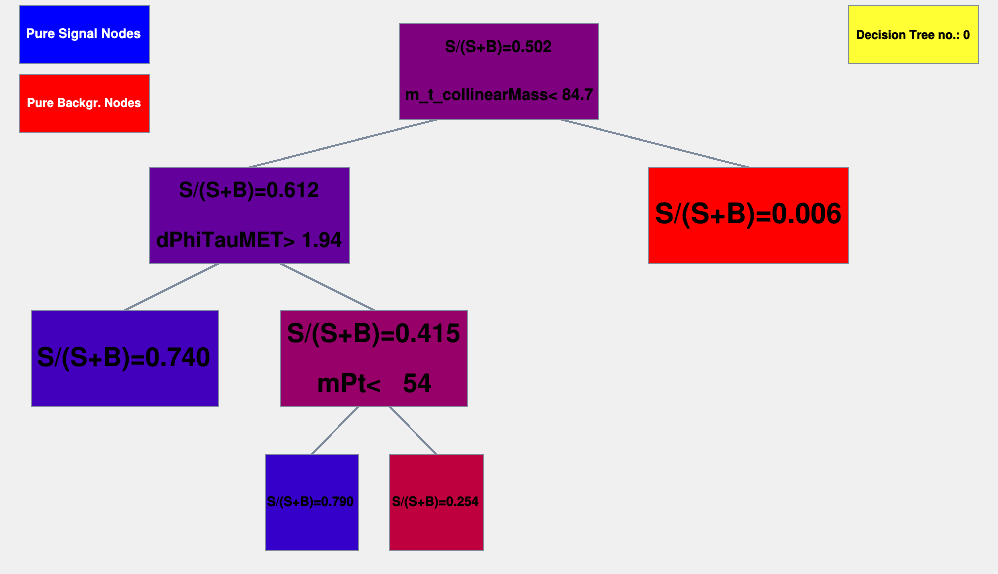
\includegraphics[width=0.8\textwidth]{plots/chapter6/BDT/BDT.png}
  \caption{Illustration of decision tree.}
  \label{fig:dec_tree}
\end{figure}

Gini Index is used as the separation criterion, and it is defined by $p.(1 - p)$, where p is the purity of the node. The purity of a node is given by the ratio of signal events to all events in that node. Since the splitting criterion is always a cut on a single variable, the training procedure selects the variable and cut value that optimizes the increase in the Gini Index between the parent node and the sum of the two daughter nodes' indices, weighted by their relative fraction of events. The same variable can thus be used for splitting several nodes, and the splitting is stopped when a predefined depth of the tree, purity of leaf nodes, the minimum number of events in a leaf node is reached. An event which ends up in a leaf node with a majority of signal events is classified as a signal event and vice versa.

A single decision tree is a weak classifier. The performance of weak classifiers can be enhanced using the Boosting technique. This technique works by building classifiers using reweighted training data and then taking a weighted majority vote of the sequence of classifiers thus produced. AdaBoost (adaptive boosting) method was used for boosting. AdaBoost is adaptive in that subsequent classifiers are tweaked in favor of those instances misclassified by previous classifiers. The misclassified event weights depend on the training error of each decision tree. The training error is calculated as

\begin{equation}
  \operatorname{err}_{m}=\frac{\sum_{i=1}^{N} w_{i} I\left(y_{i} \neq DT_{m}\left(x_{i}\right)\right)}{\sum_{i=1}^{N} w_{i}}
\end{equation}

in which the subscript m is the tree label and w is the event weight. The $y_{i}$ is the true label for the event, 1 for signal and -1 for background. $DT_{m}(x_{i})$ is the output of the decision tree. The variable $I(y_{i} \neq DT_{m}(x_{i}))$ equals 1 if $y_{i} \neq DT_{m}(x_{i})$ or 0 otherwise. The weight for event i is updated using $\alpha_{m}$ which is calculated from the training error. $\beta$ is the learning rate.

\begin{align}
  \alpha_{m}=\beta \times \ln \left(\left(1-\operatorname{err}_{m}\right) / \operatorname{err}_{m}\right) \\
  w_{i} \rightarrow w_{i} \times e^{\alpha I\left(y_{i} \neq DT_{m}\left(x_{i}\right)\right)}
\end{align}

By construction, the training error is $err_{m} \leq 0.5$ as the same training events used to classify the output nodes of the previous tree are used to calculate the training error. The learning rate parameter can be used to adjust the step size of each re-weighting. Event weights in each tree are renormalized to keep the summed weights constant. After the boosting and training processes, the final score of each event is $DT(x)$. A high score indicates a signal like event while a low score indicates a background like event.

\begin{equation}
DT(x)=\sum_{m=1}^{N_{tree}} \alpha_{m} DT_{m}(x)
\end{equation}

This technique also helps in stabilizing the response of the classifiers for fluctuations in the training data. It utilizes a predefined depth of the tree instead of pruning it to avoid overfitting to the training data. All the BDT trainings were done with an ensemble of 850 decision trees, with each tree having a maximum depth of 3. The minimum node size is required to be 2.5\%, and the learning rate is set to 0.5. A training to testing split of 50:50 was used.

\section{\texorpdfstring{\Hmuhad}{Hmutauh} channel}
The first step is to require the events to pass an isolated muon trigger. For 2016 data, this trigger has a muon \pt\, threshold of 24\GeV. However, for the 2017 and 2018 data, the trigger with a 24\GeV threshold is prescaled.  Prescaling corresponds to collecting one out of every n events to reduce the event rate. We use this trigger in conjunction with the isolated muon trigger with a muon \pt\, threshold of 27\GeV. In addition to the event passing the trigger, the reconstructed leptons corresponding to the trigger have to match the HLT objects within $\Delta R < 0.5$.

Next, the preselection begins by requiring an isolated \Pgm\, and an isolated \tauh candidates of opposite electric charge and separated by $\Delta\text{R} > 0.5$. The muon candidate is required to have $\pt > 26\GeV$, $\abs{\eta} < 2.1$ and isolation $I^{\Pgm}_\text{rel} < 0.15$. The \tauh candidate is required to have $\pt > 30\GeV$ and $\abs{\eta} < 2.3$. Events containing additional electrons, muons, or \tauh candidates are vetoed. Events with at least one b jet tagged by DeepCSV algorithm are rejected in order to suppress the \ttbar background.

A BDT is trained after applying preselection criteria. The signal training sample considered is a mixture of simulated GGF and VBF events, weighted according to their respective SM production cross-sections. The misidentified lepton background and \Ztt background are the dominant backgrounds in this channel. The background used for training the BDT is a data sample of misidentified lepton events with the same charge assignment for both leptons along with the Drell-Yan MC sample with signal selections. The input variables to the BDT are $\pt^{\Pgm}, \pt^{\tauh}$, \mcol, \ptvecmiss, \mt(\tauh, \ptvecmiss), \detamtauh, \dphimtauh, and \dphitauhmet. The distribution of the input variables to the BDT can be seen in Figure ~\ref{fig:input_mt}.

\begin{figure}[htbp!]
  \centering
  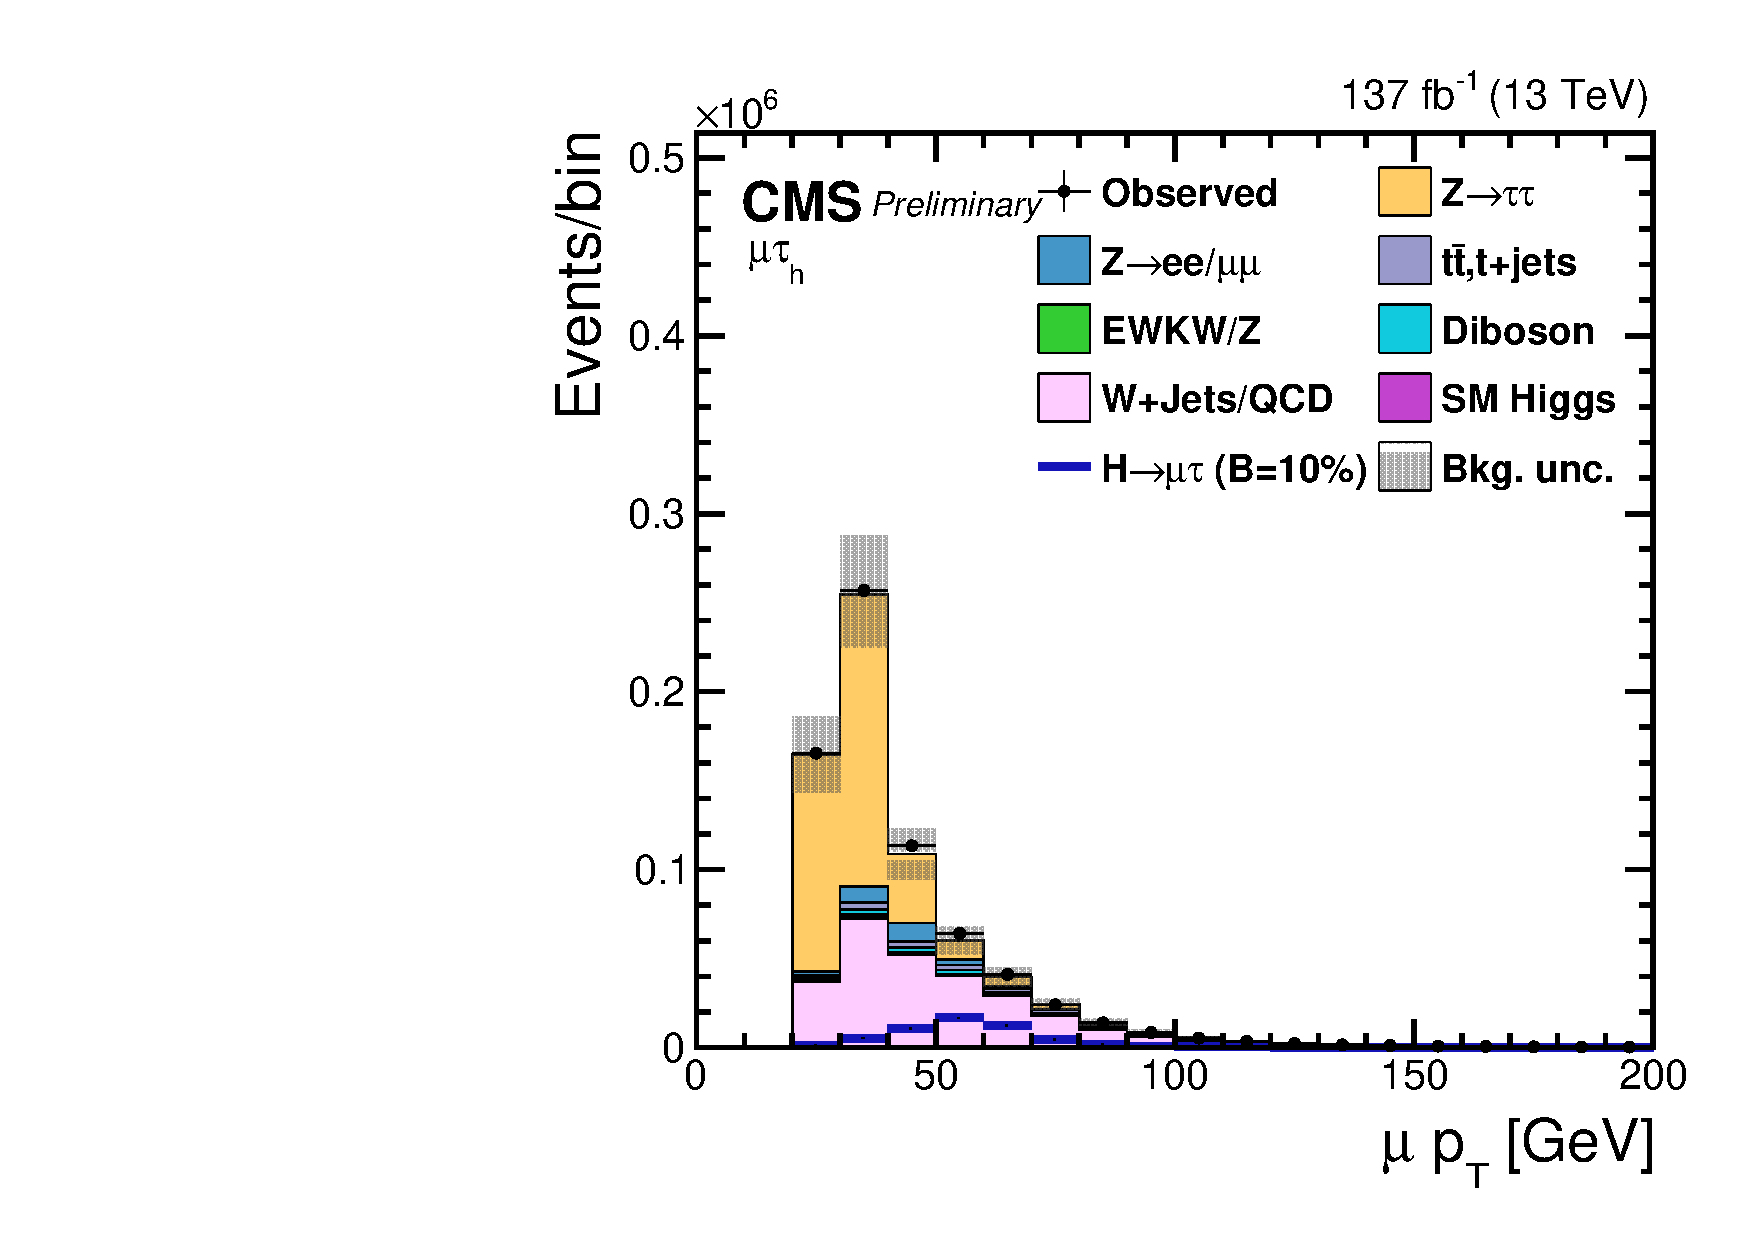
\includegraphics[width=0.36\textwidth]{plots/chapter6/mutau/mPt.pdf}
  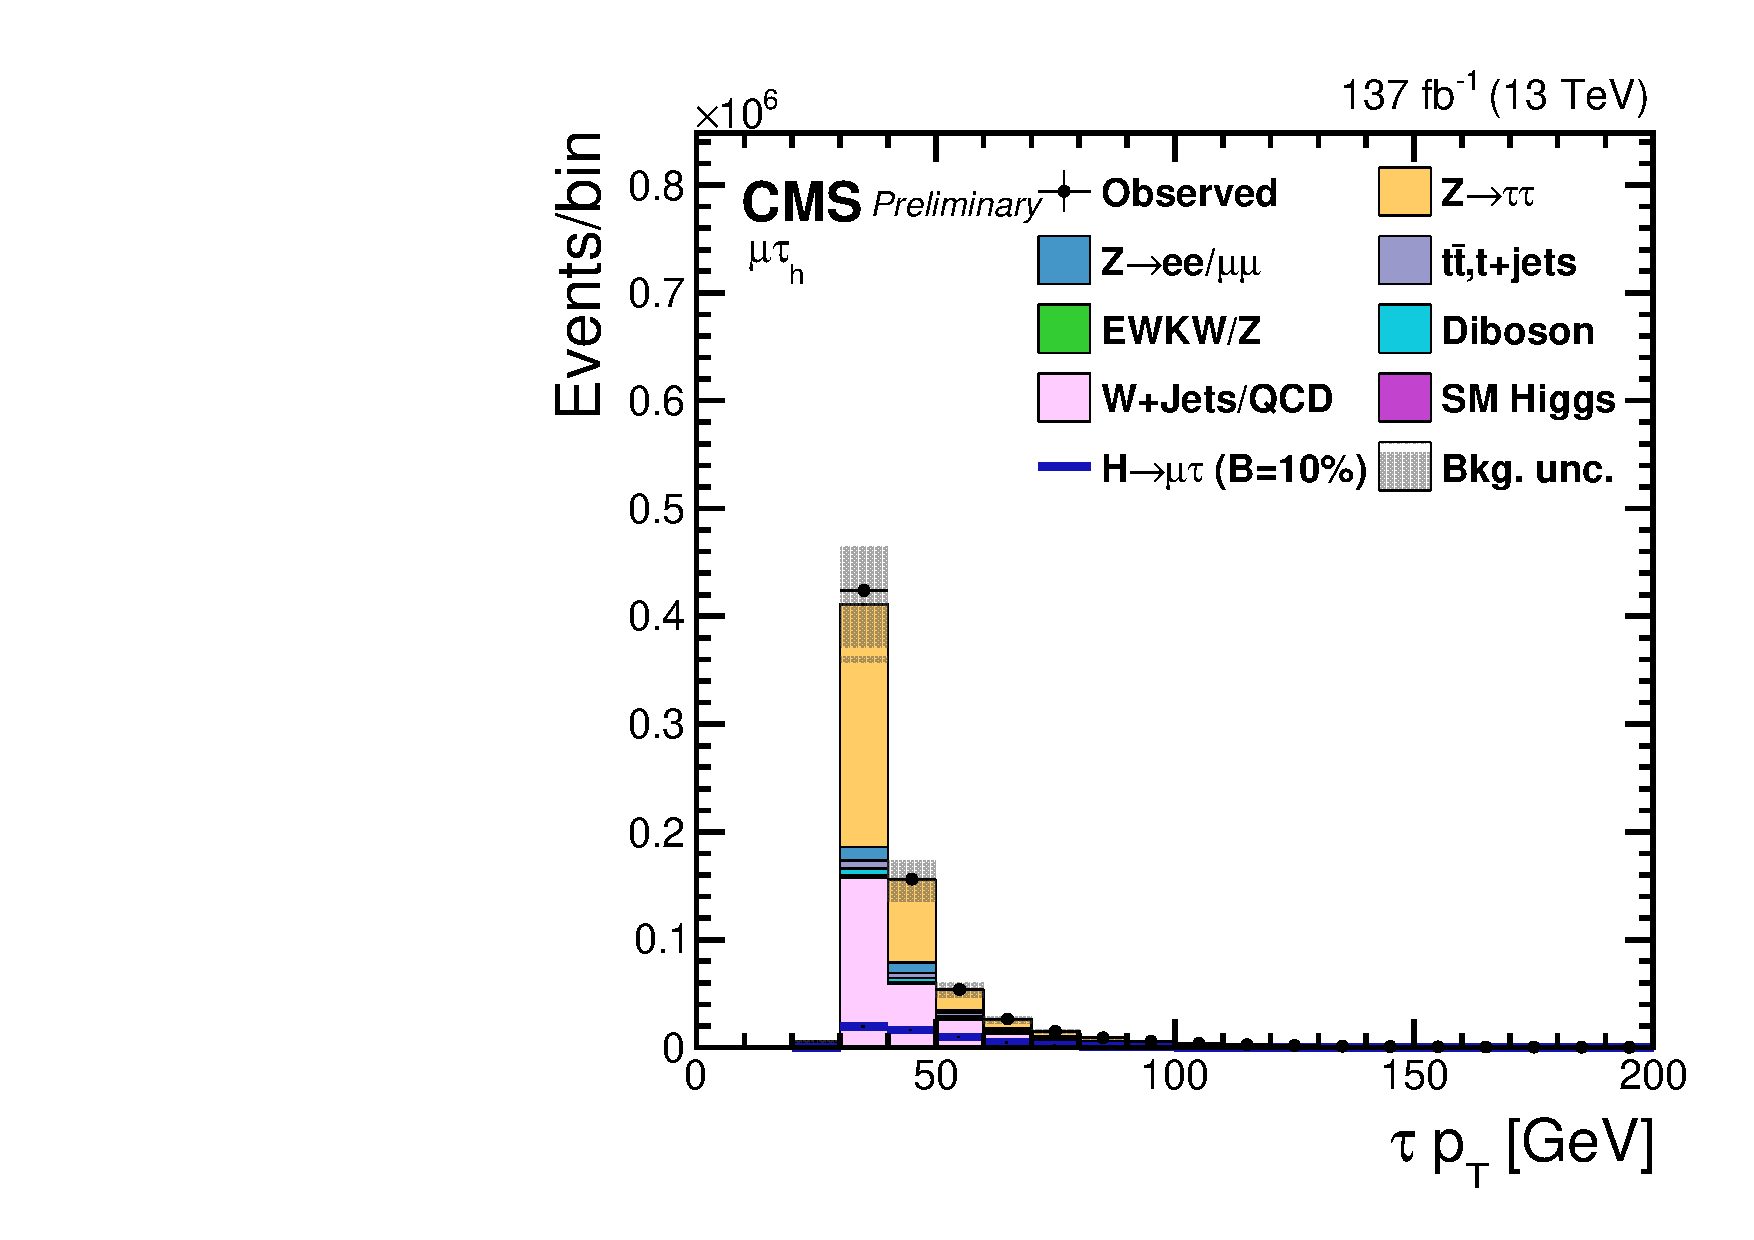
\includegraphics[width=0.36\textwidth]{plots/chapter6/mutau/tPt.pdf}\\
  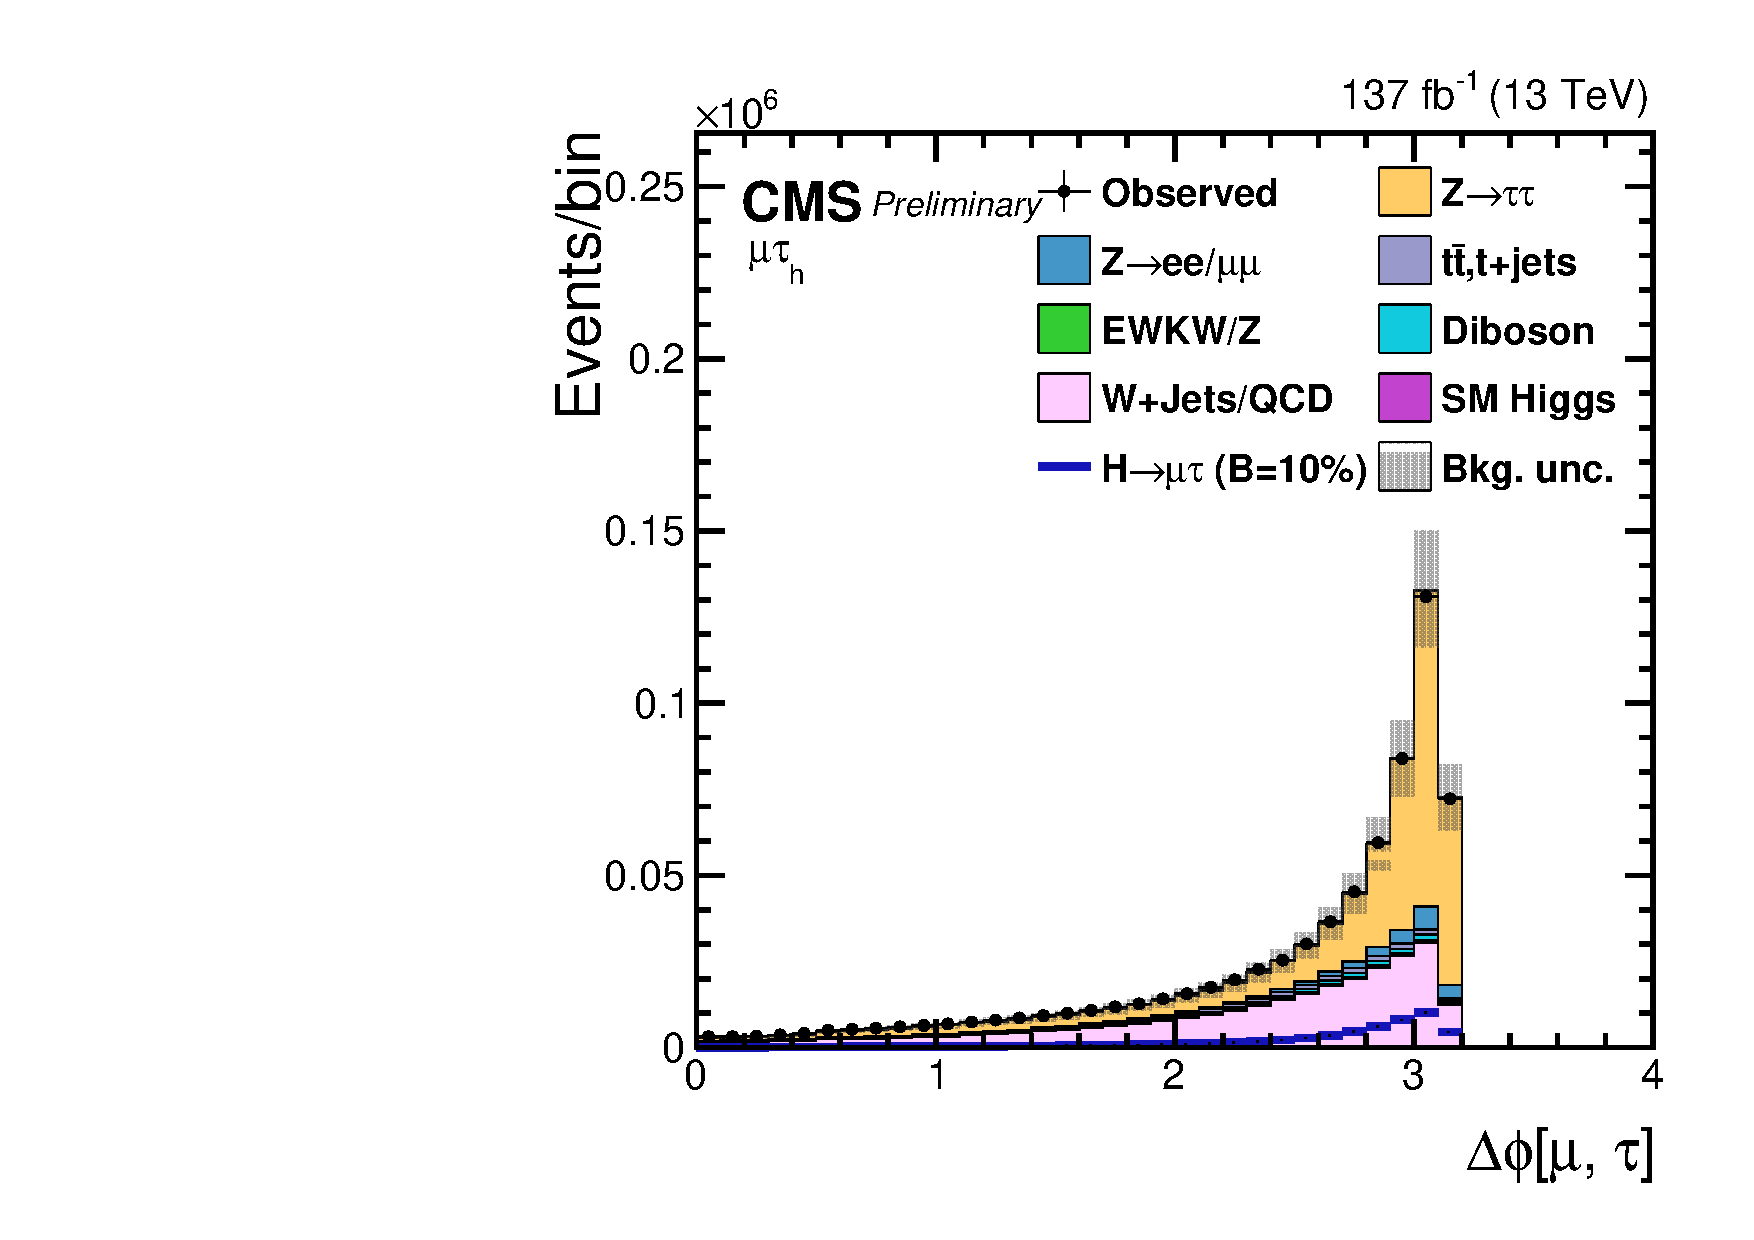
\includegraphics[width=0.36\textwidth]{plots/chapter6/mutau/dPhiMuTau.pdf}
  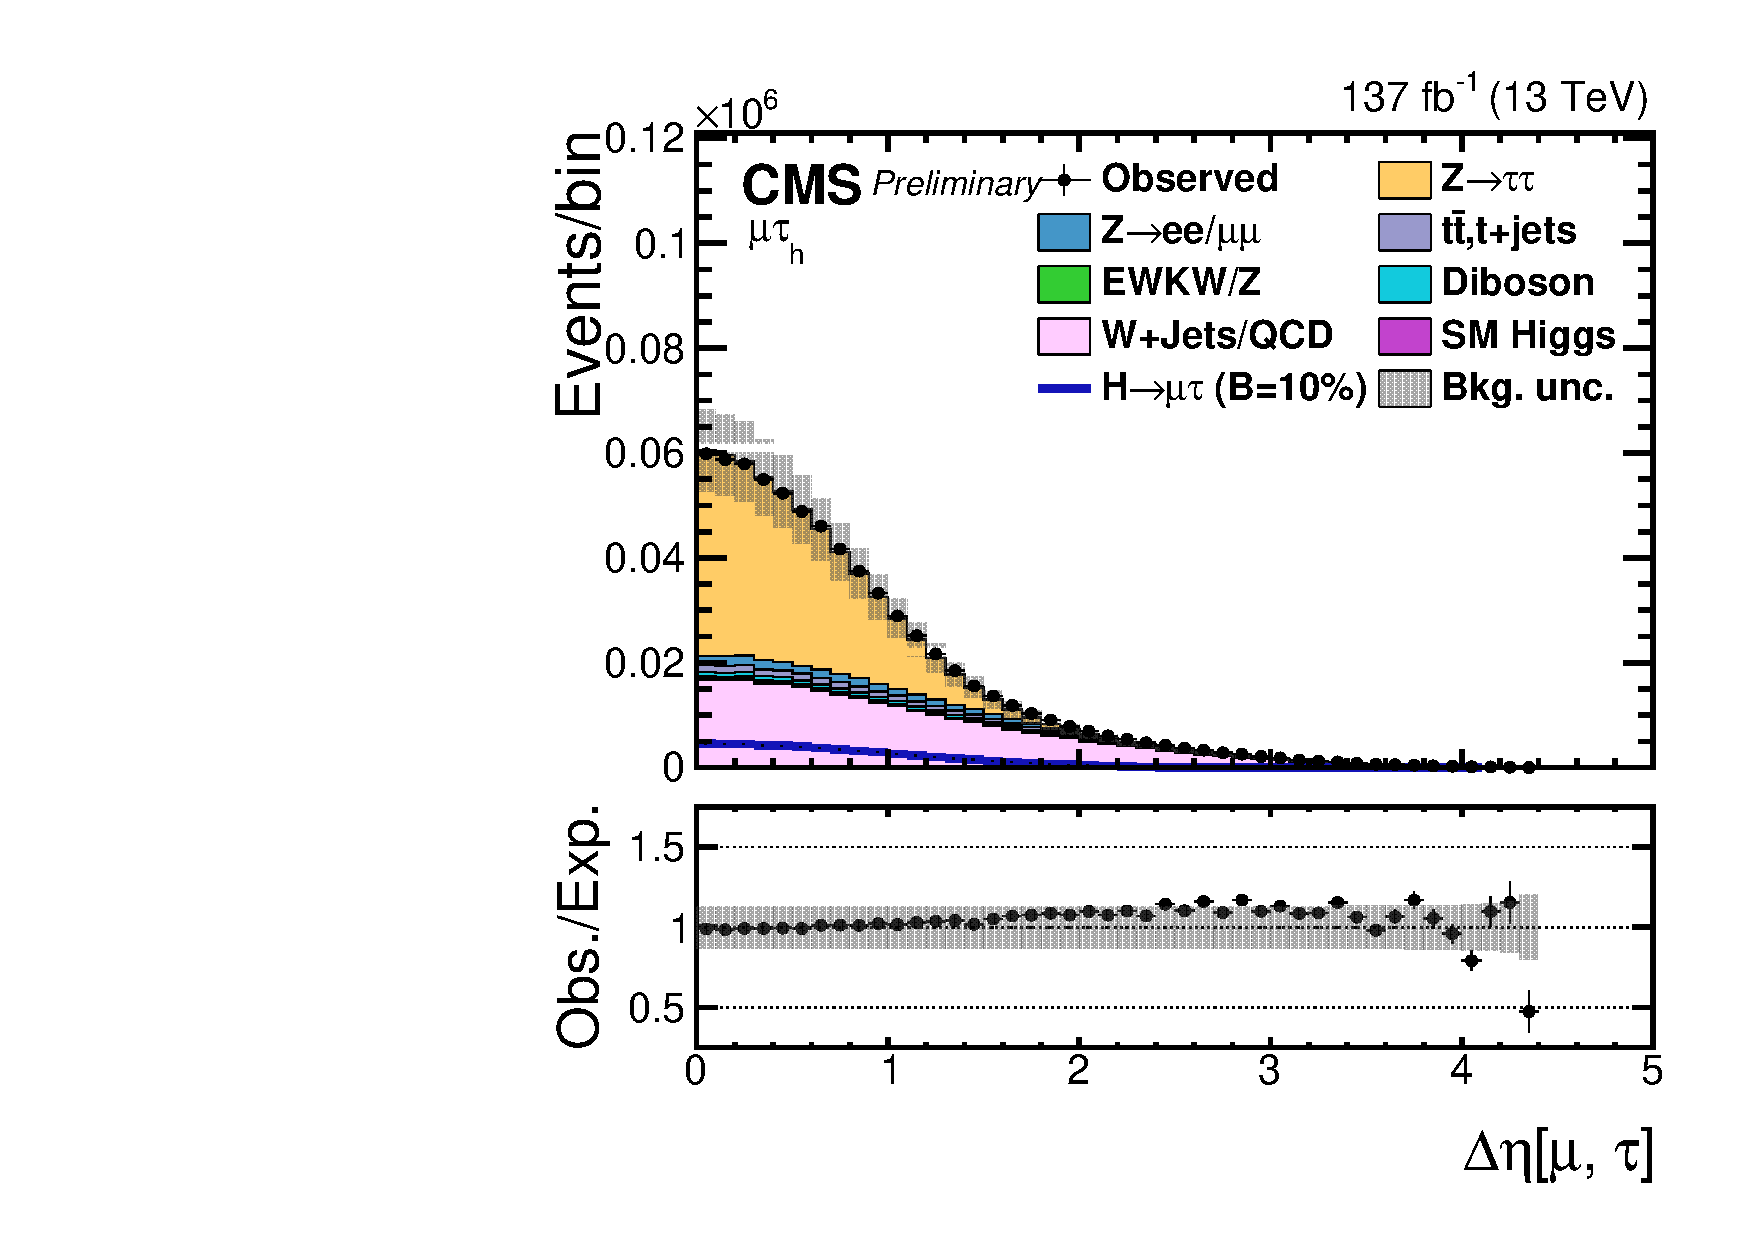
\includegraphics[width=0.36\textwidth]{plots/chapter6/mutau/dEtaMuTau.pdf}\\
  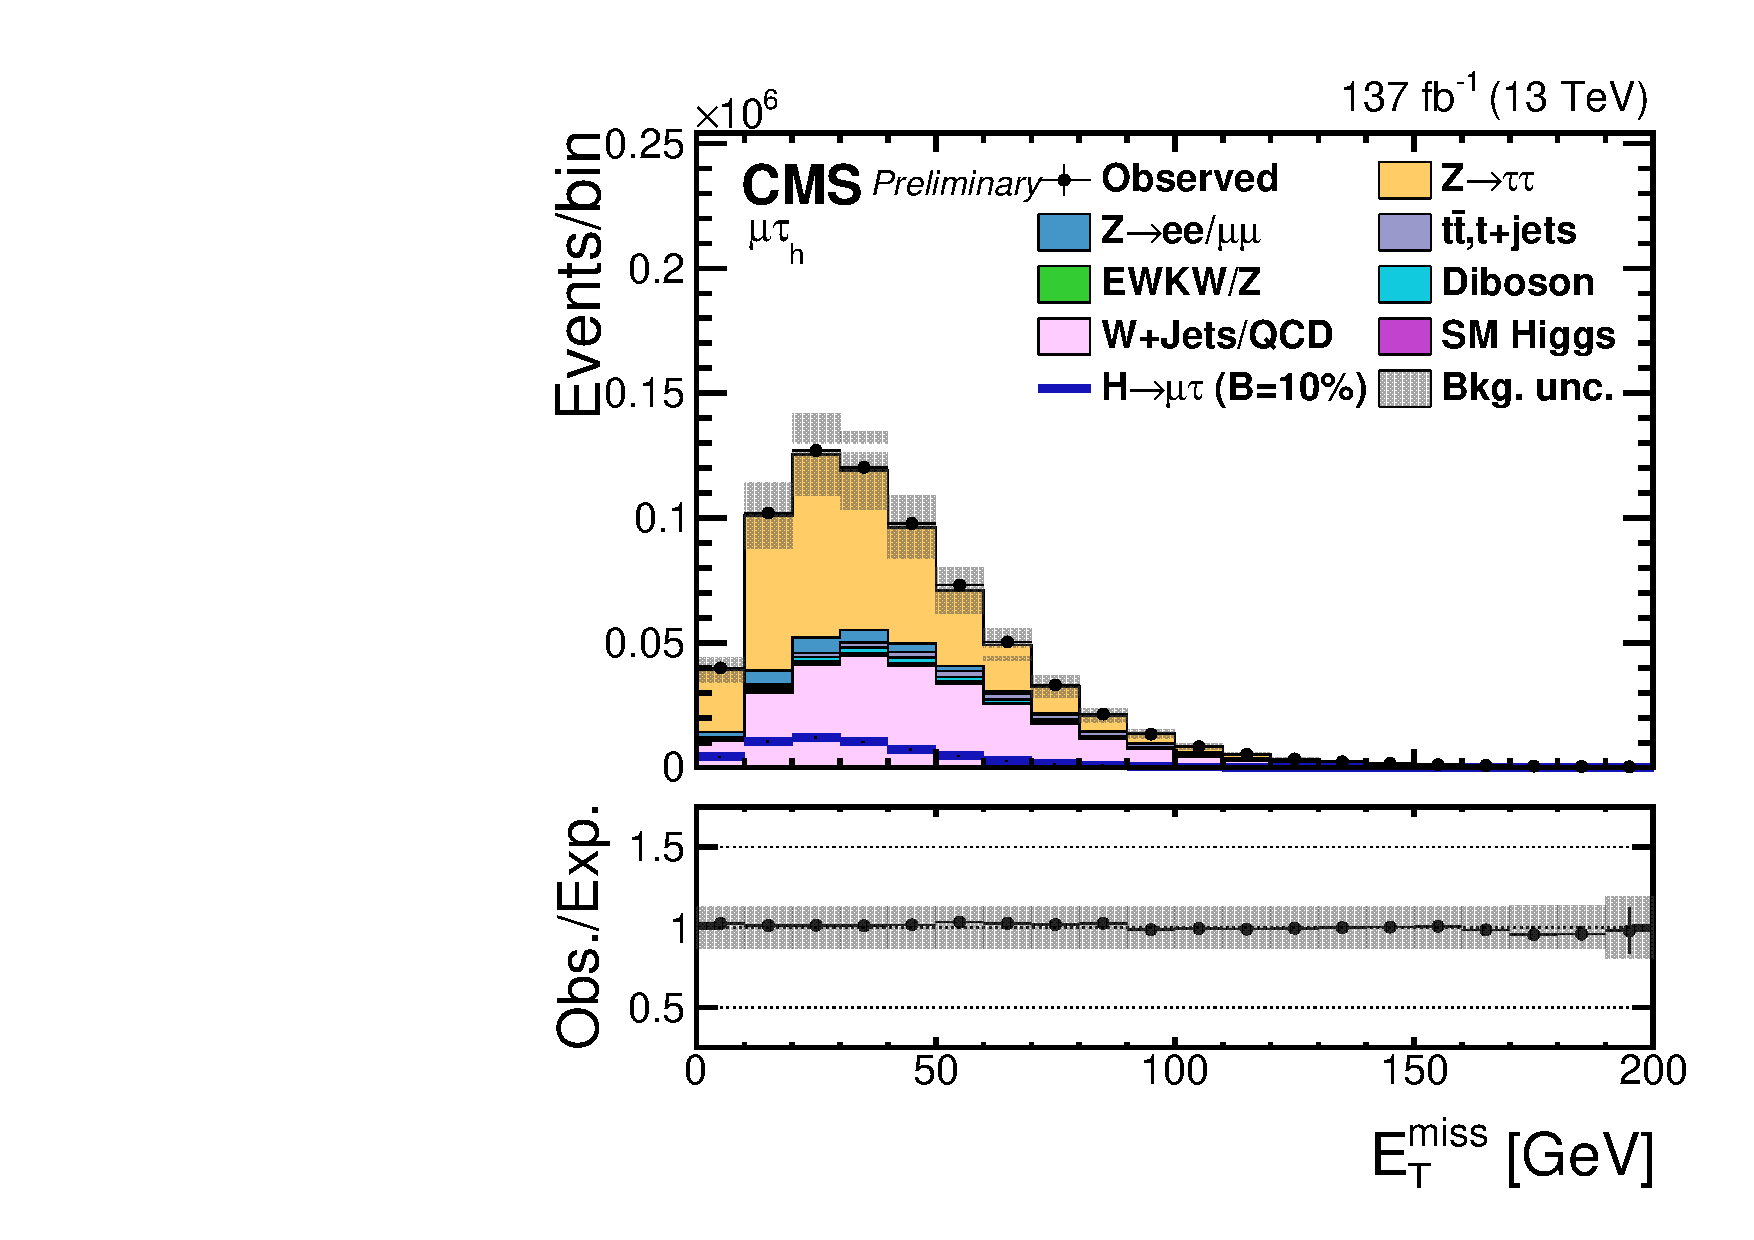
\includegraphics[width=0.36\textwidth]{plots/chapter6/mutau/type1_pfMetEt.pdf}
  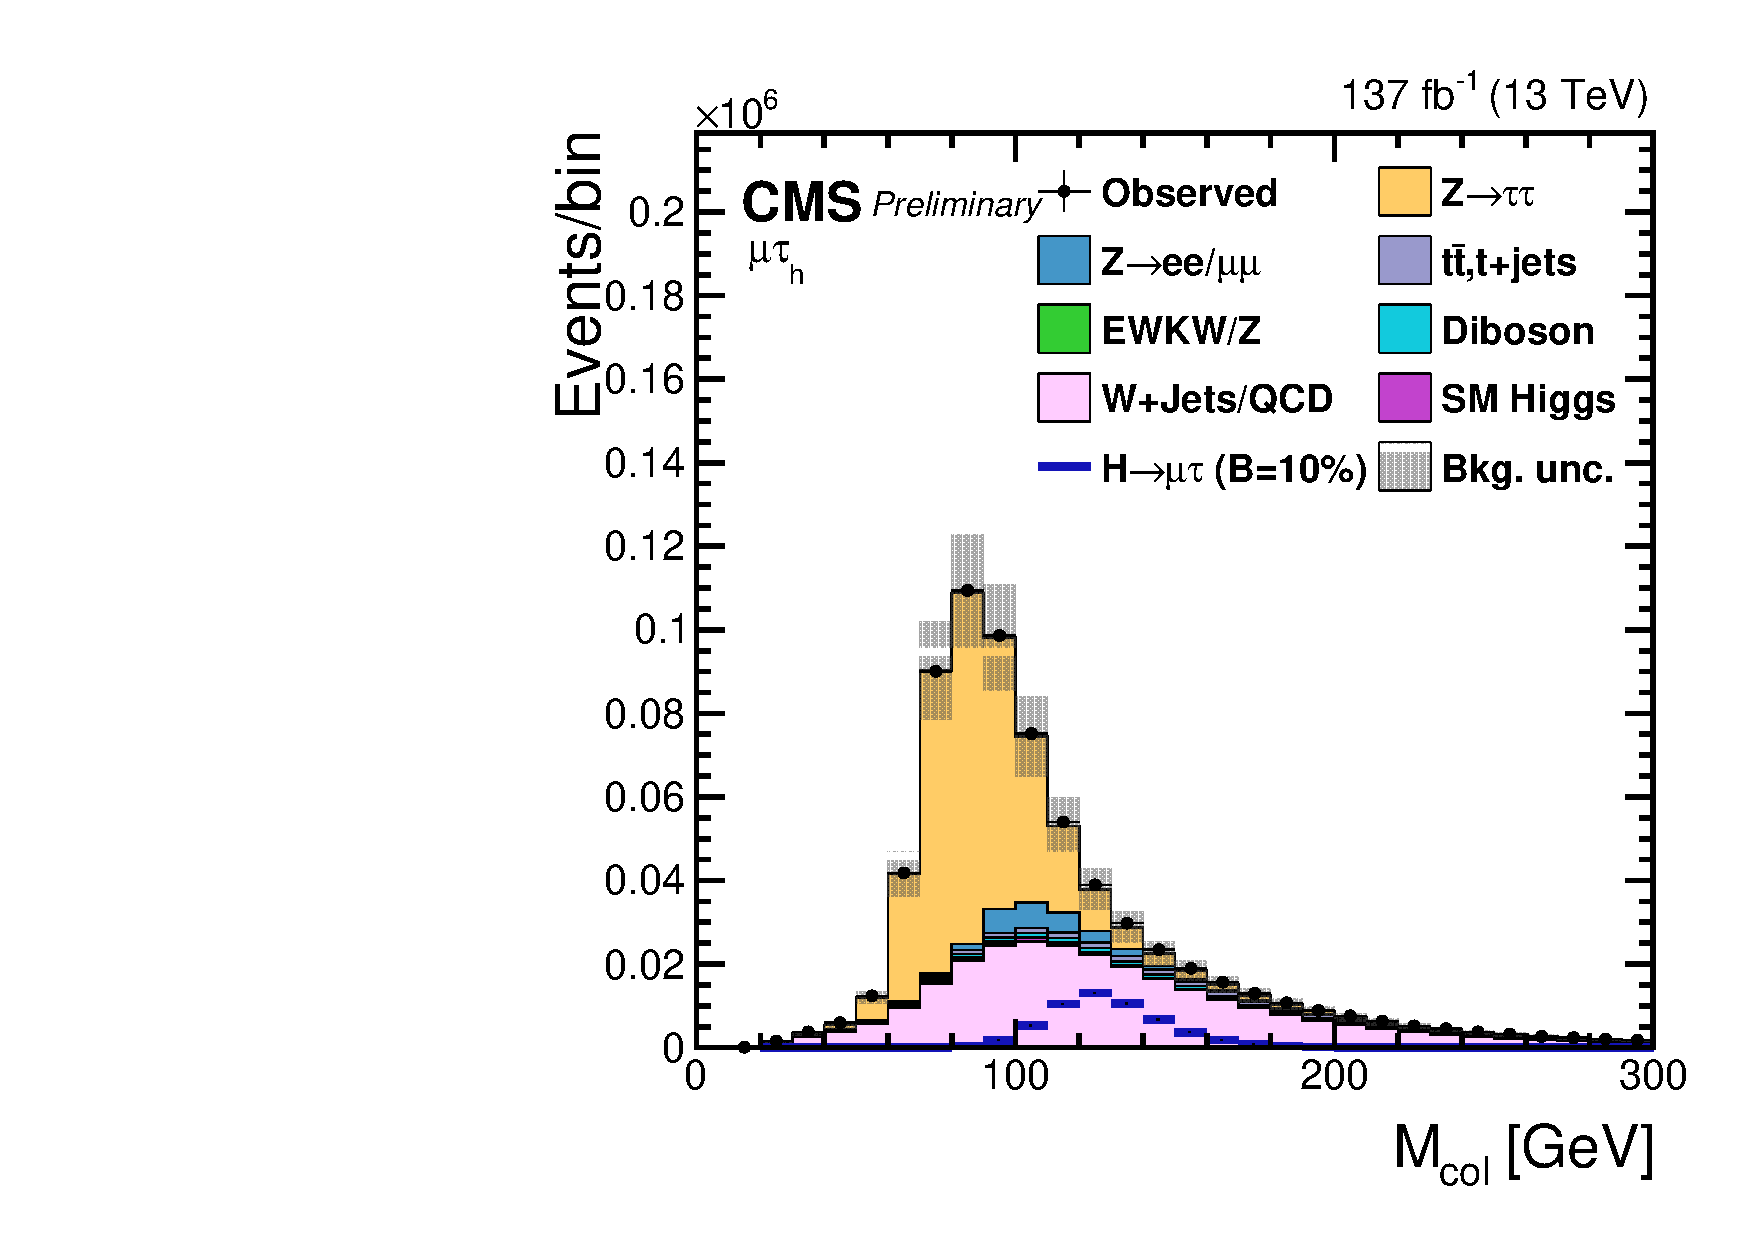
\includegraphics[width=0.36\textwidth]{plots/chapter6/mutau/m_t_CollinearMass.pdf}\\
  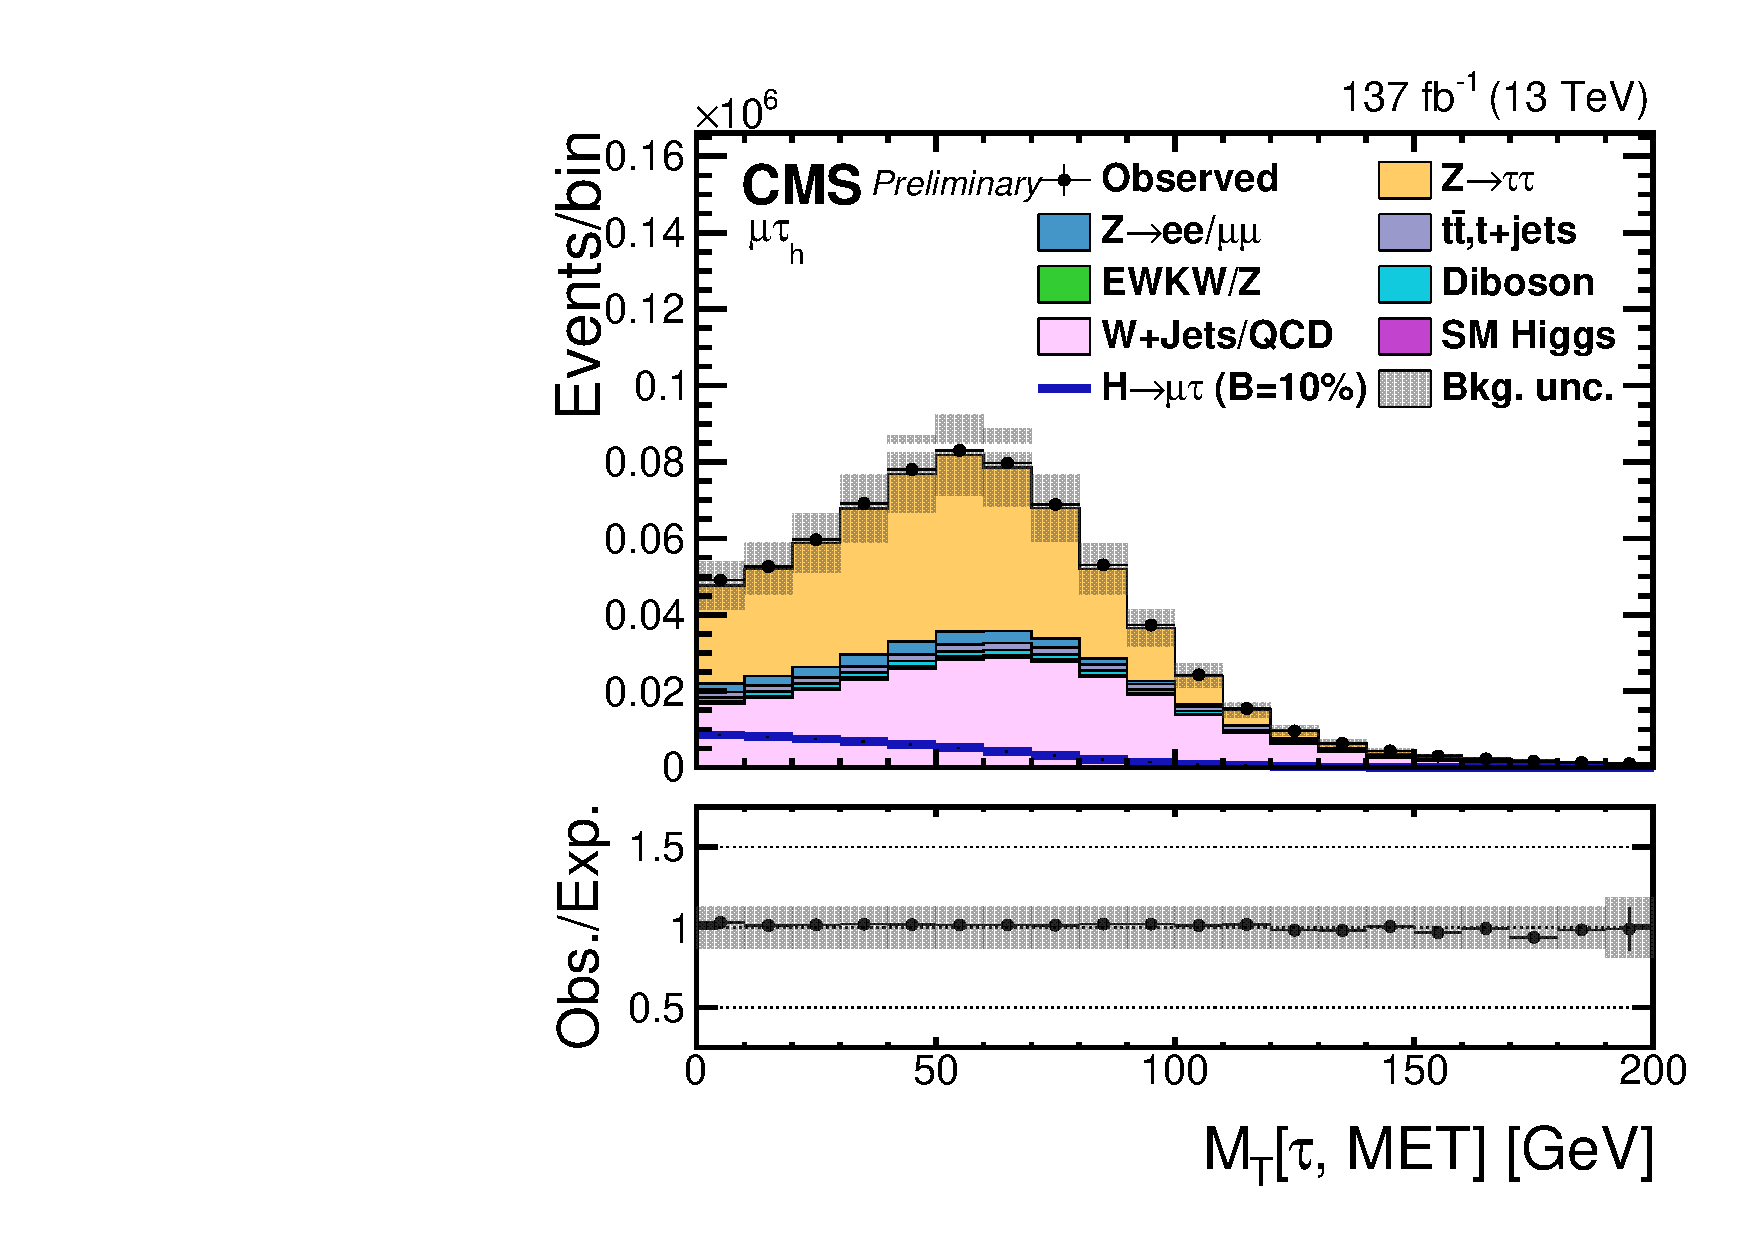
\includegraphics[width=0.36\textwidth]{plots/chapter6/mutau/MTTauMET.pdf}
  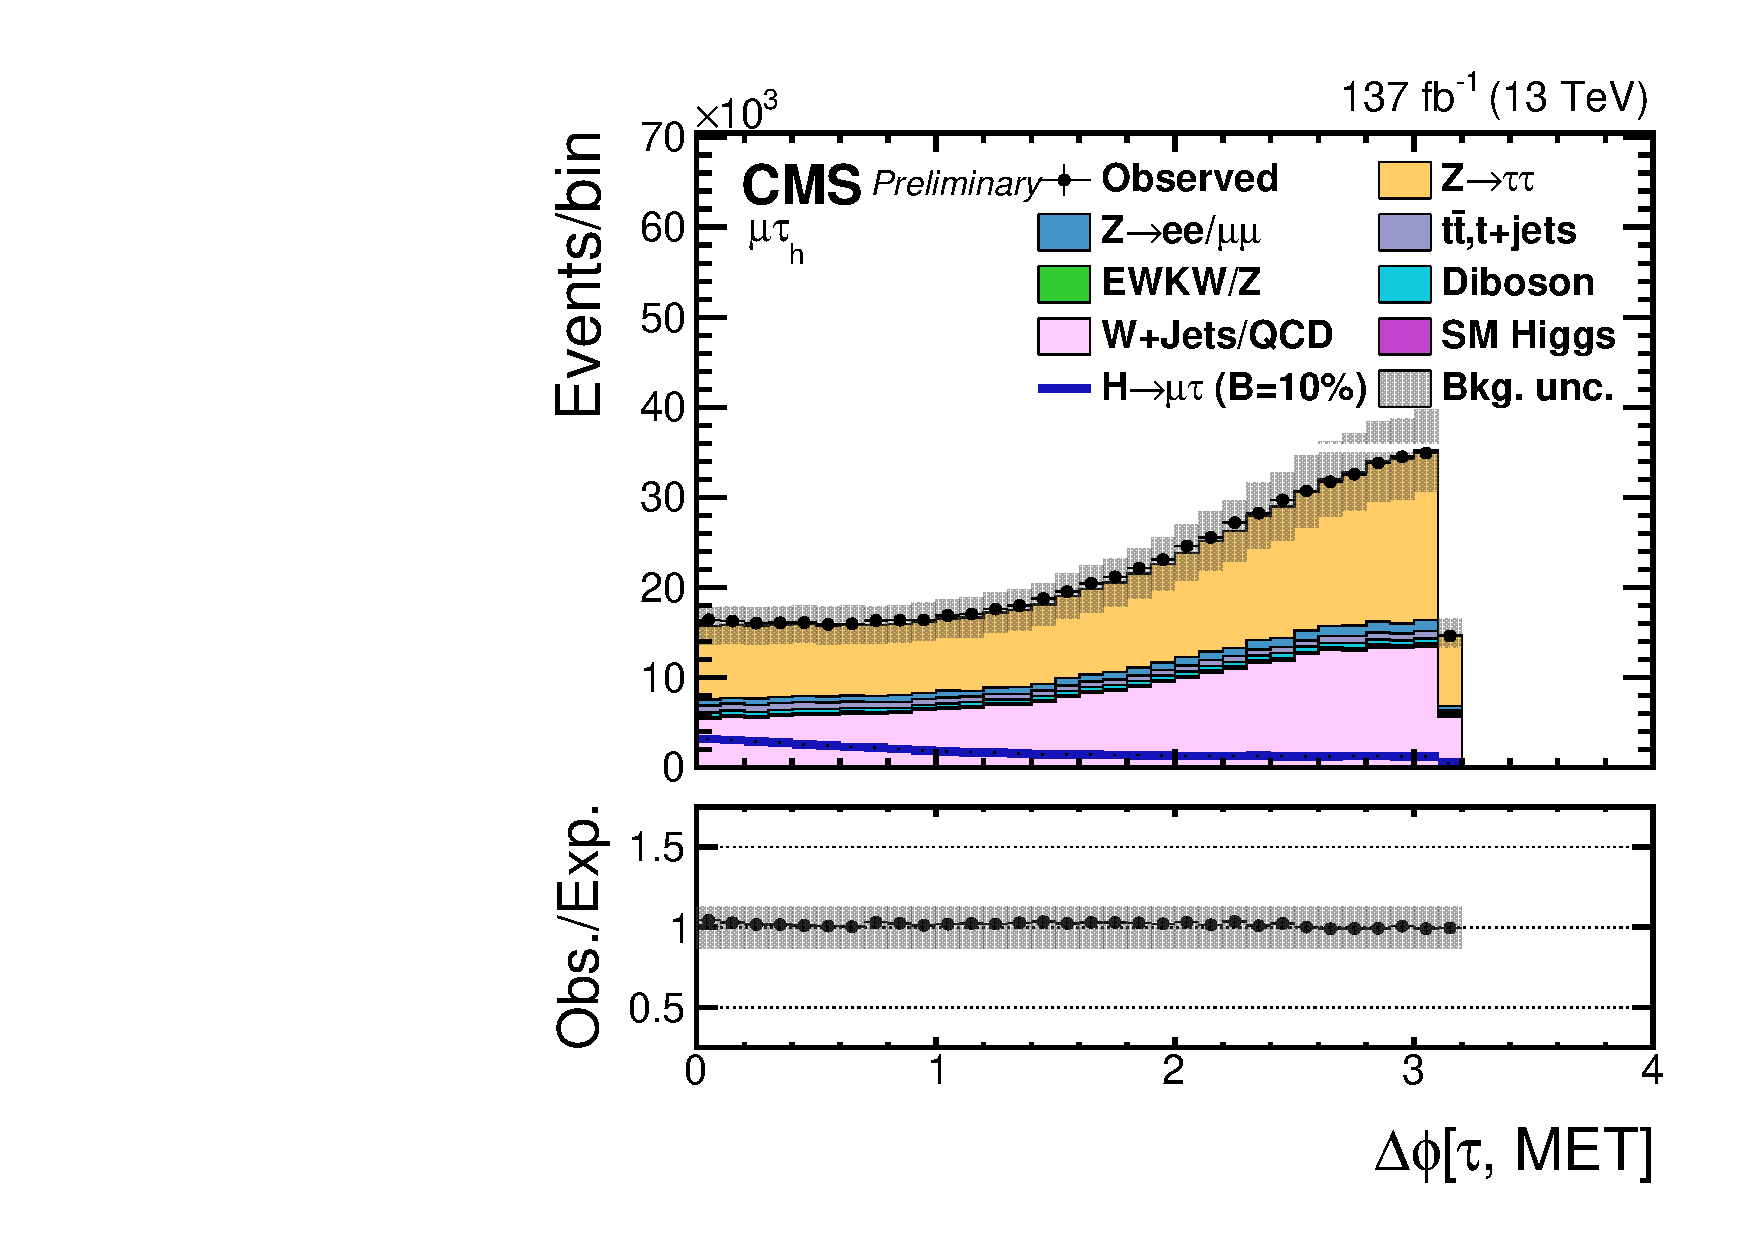
\includegraphics[width=0.36\textwidth]{plots/chapter6/mutau/dPhiTauMET.pdf}\\
  \caption{Distribution of the input variables to the BDT for the \Hmuhad process.}
  \label{fig:input_mt}
\end{figure}

The selection on \ptvecmiss is motivated by the presence of neutrinos in the \Pgt\, lepton decays. The neutrino is expected to be collinear with \tauh, which leads to selection on the \dphitauhmet variable. The two leptons are usually in the opposite direction in the azimuthal plane, which leads to selection on the \dphimtauh variable. The BDT discriminator distributions of simulated signal, data, and backgrounds for each category in \Hmuhad channel, are shown in results chapter.

In the \mcol fit method, additional selection criteria require $\mt(\tauh, \ptvecmiss) < 105\GeV$ in the $0-, 1-,$ and $2-$jet GGF categories and $\mt(\tauh, \ptvecmiss) < 85\GeV$ in the $2-$jet VBF category. The \mcol distributions of simulated signal, data, and backgrounds for each category in \Hmuhad channel, are shown in results chapter.

\begin{figure}[htbp]
  \centering
  \subfigure[]{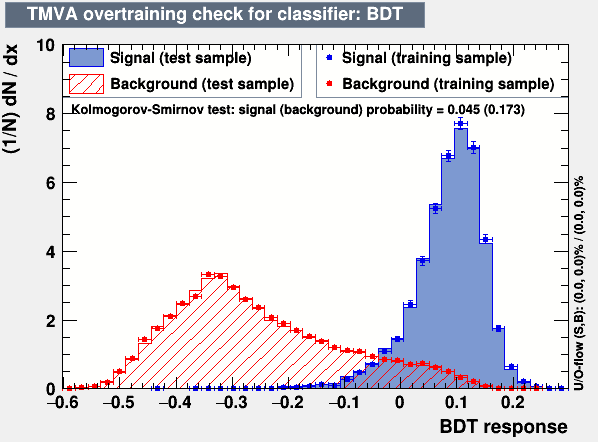
\includegraphics[width=0.32\textwidth]{plots/chapter6/BDT/mutau/2016.png}}
  \subfigure[]{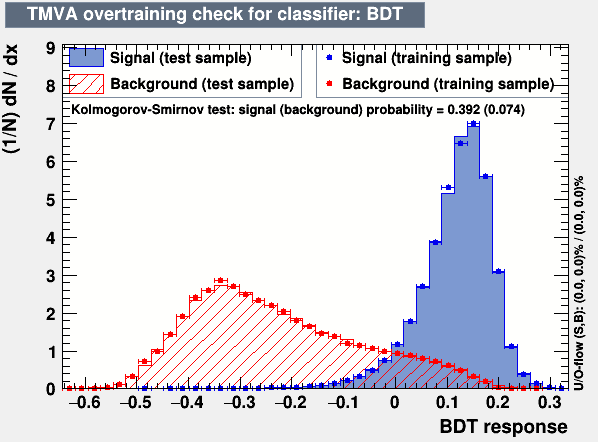
\includegraphics[width=0.32\textwidth]{plots/chapter6/BDT/mutau/2017.png}}
  \subfigure[]{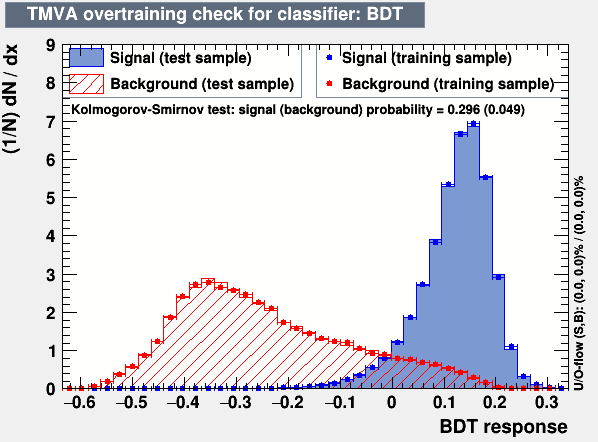
\includegraphics[width=0.32\textwidth]{plots/chapter6/BDT/mutau/2018.png}}
  \caption{Overtraining check as performed in TMVA for the trained BDT in \Hmuhad channel for 2016 (a), 2017 (b), and 2018 (c).}
  \label{fig:mutauh_bdttrain}
\end{figure}

%%% MU-TAU event selection
\begin{table}[!hbpt]
\centering
\caption{Event selection criteria for the kinematic variables for the \Hmt channels}
\begin{tabular}{lccccccccc}
\hline
Variable                       &       \multicolumn{4}{c}{\muhad}            & &          \multicolumn{4}{c}{\mue}                    \\
\hline
$\pt^{\Pe}$                    &       \multicolumn{4}{c}{\NA}               & &          \multicolumn{4}{c}{$>13$}                   \\
$\pt^{\Pgm}$                   &       \multicolumn{4}{c}{$>26$}             & &          \multicolumn{4}{c}{$>24$}                   \\
$\pt^{\tauh}$                  &       \multicolumn{4}{c}{$>30$}             & &          \multicolumn{4}{c}{\NA}                     \\
\hline
$\abs{\eta}^{\Pe}$             &       \multicolumn{4}{c}{\NA}               & &          \multicolumn{4}{c}{$<2.5$}                  \\
$\abs{\eta}^{\Pgm}$            &       \multicolumn{4}{c}{$<2.1$}            & &          \multicolumn{4}{c}{$<2.4$}                  \\
$\abs{\eta}^{\tauh}$           &       \multicolumn{4}{c}{$<2.3$}            & &          \multicolumn{4}{c}{\NA}                     \\
\hline
$I^{\Pe}_{\text{rel}}$         &       \multicolumn{4}{c}{\NA}               & &          \multicolumn{4}{c}{$<0.1$}                  \\
$I^{\Pgm}_{\text{rel}}$        &       \multicolumn{4}{c}{$<0.15$}           & &          \multicolumn{4}{c}{$<0.15$}                 \\
$I^{\tauh}_{\text{rel}}$       &       \multicolumn{4}{c}{DNN \tauh ID}      & &          \multicolumn{4}{c}{\NA}                     \\
\hline
Trigger                        &    \multicolumn{4}{c}{\Pgm(24) (all years)} & & \multicolumn{4}{c}{\Pe(12) and \Pgm(23) (all years)} \\
\hline \\

                               &                          \multicolumn{9}{c}{\mcol fit selection}                                     \\
\cline{2-10}
                               & 0-jet  & 1-jet  & \multicolumn{2}{c}{2-jet} & & 0-jet  & 1-jet  & \multicolumn{2}{c}{2-jet}          \\
\cline{2-5} \cline{7-10}
                               &        &        &   ggF       &      VBF    & &        &        &   ggF       &      VBF             \\
\hline
\mjj                           &   \NA    &   \NA    &  $<550$   & $\geq550$ & &    \NA    &    \NA    &  $<550$   &  $\geq550$       \\
\hline
$\pt^{\Pgm}$                   &          \multicolumn{4}{c}{\NA}            & &   $>30$   &   $>26$   &   $>26$   &   $>26$          \\
\mt(\Pgm)                      &          \multicolumn{4}{c}{\NA}            & &   $>60$   &   $>40$   &   $>15$   &   $>15$          \\
\mt(\Pgt)                      &  $<105$  &  $<105$  &  $<105$   &   $<85$   & &           \multicolumn{4}{c}{\NA}                    \\
\dphiemet                      &          \multicolumn{4}{c}{\NA}            & &   $<0.7$  &   $<0.7$  &   $<0.5$  &   $<0.3$         \\
\dphiem                        &          \multicolumn{4}{c}{\NA}            & &   $>2.5$  &   $>1.0$  &    \NA    &    \NA           \\
\hline
\end{tabular}
\label{tab:mutau_evtselection}
\end{table}


\section{\texorpdfstring{\Hmue}{Hmutaue} channel}
The events are required to pass the cross-trigger with \pt\, thresholds on the muon and the electron. The \pt\, threshold on the muon is 23\GeV, and on the electron is 12\GeV. The cross-trigger also places a constraint on the two leptons' longitudinal impact parameter to the primary vertex. However, this constraint is not present in the initial 2016 data samples and 2016 MC samples. In addition to the event passing the trigger, the reconstructed leptons corresponding to the trigger have to match the HLT objects within $\Delta R < 0.5$.

The preselection criteria for \Hmue channel requires an isolated muon and an isolated electron candidates of opposite charge and separated by $\Delta\text{R} > 0.3$. The muon candidate is required to have $\pt > 24\GeV$, $\abs{\eta} < 2.4$ and isolation $I^{\Pgm}_\text{rel} < 0.15$. The electron candidate is required to have $\pt > 13\GeV$, $\abs{\eta} < 2.5$ and isolation $I^{\Pe}_\text{rel} < 0.1$. The \pt\, thresold of the electron and the muon are dictated by the cross-trigger we use for selecting the events of this channel. Events containing additional electrons, muons, \tauh candidates or at least one b jet tagged by DeepCSV algorithm are removed.

Similar to the \Hmuhad channel, a BDT is trained after applying preselection criteria. The signal training is done in a similar way while for background training dominant contributors, \ttbar and \Zll ($\ell=\Pe, \Pgm, \Pgt$) events are mixed and weighted by their respective production cross-sections. The \ttbar process contributes dominantly for the $2-$jet category, with significant contribution to $1-$jet category. \Zll background processes dominantly contribute the $0-$ and $1-$jet categories. The QCD multijet background has the third-largest contribution, so we use the same sign control region in data as additional background for training. The input variables to the BDT are: $\pt^{\Pgm}, \pt^{\Pe}$, \mcol, \mt(\Pgm, \ptvecmiss), \mt(\Pe, \ptvecmiss), \dphiem, \dphimmet, and \dphiemet. The distribution of the input variables to the BDT can be seen in Figure ~\ref{fig:input_me}. The BDT discriminator distributions of simulated signal, data, and backgrounds for each category in \Hmue channel, are shown in results chapter.

\begin{figure}[htbp!]
  \centering
  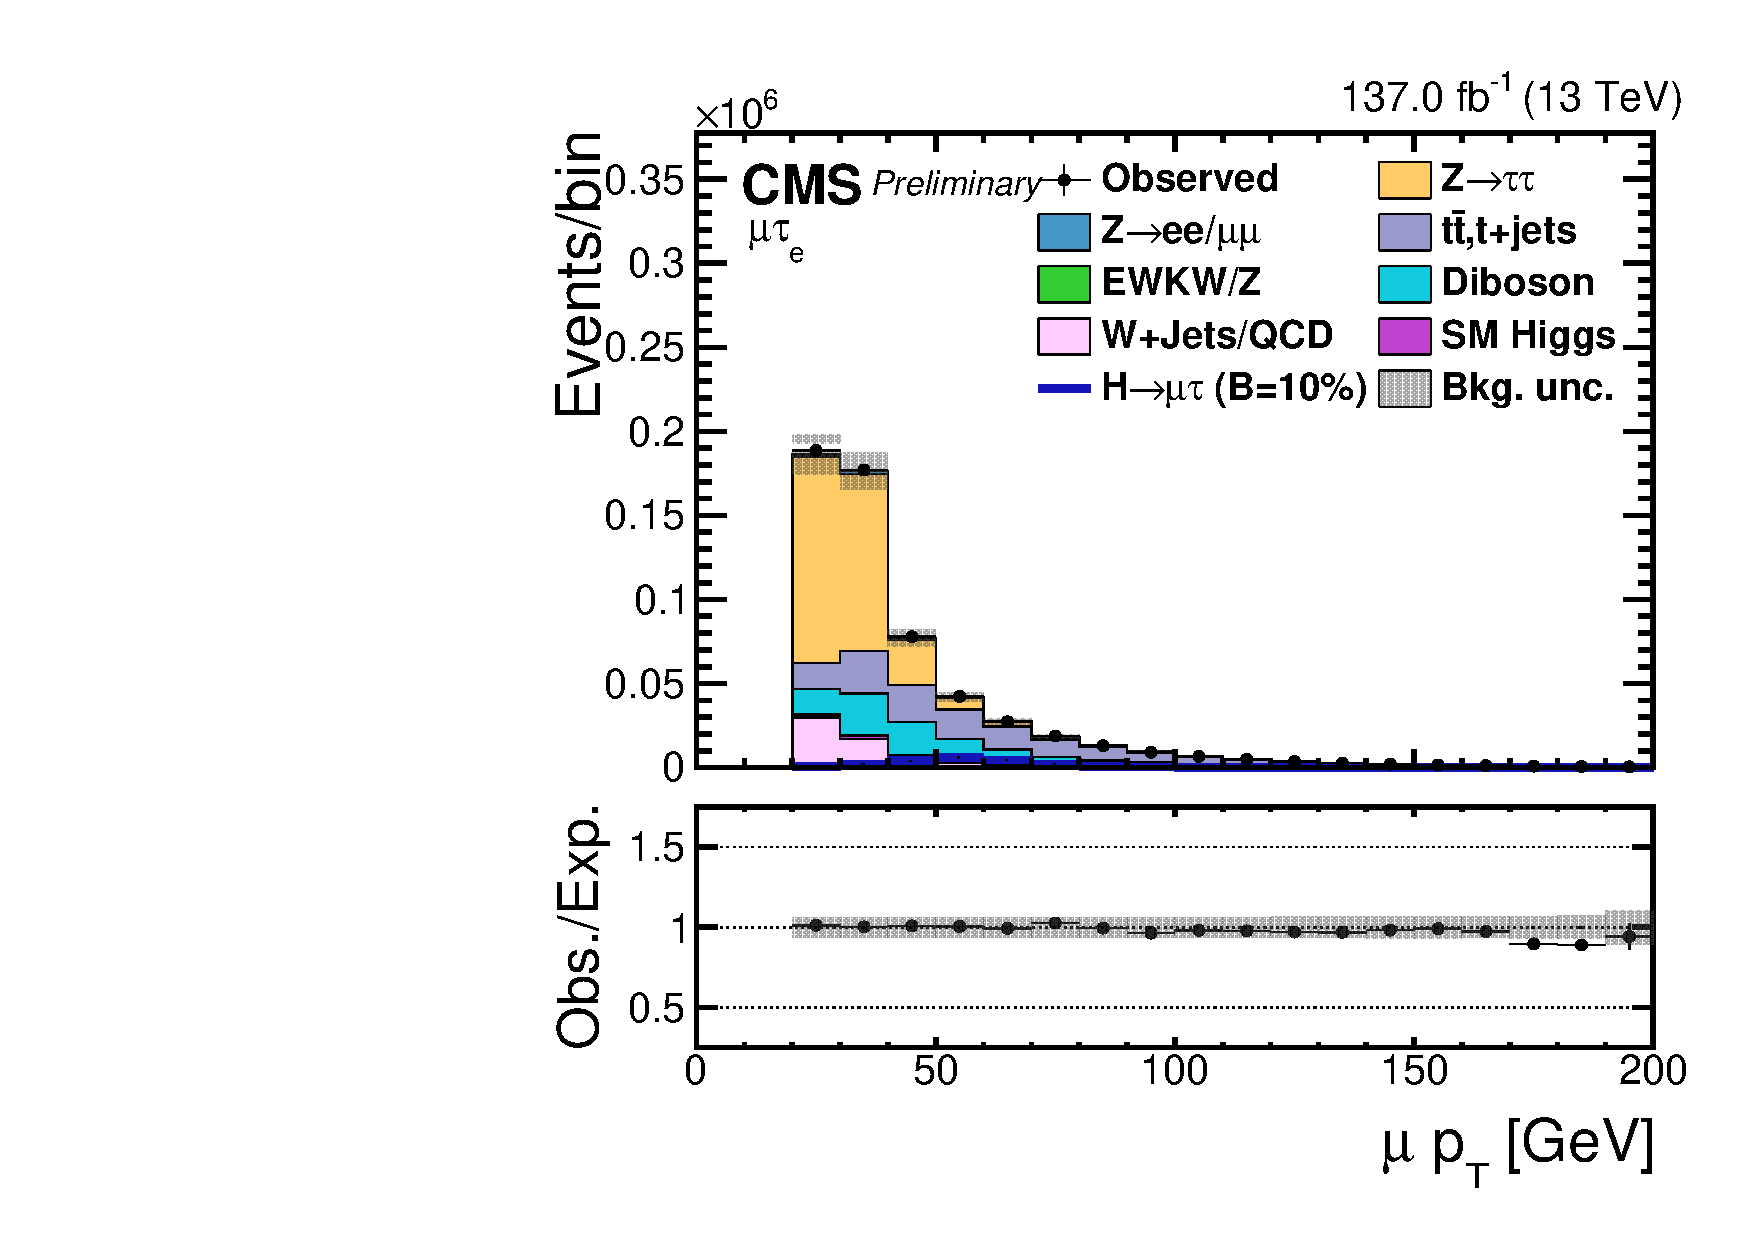
\includegraphics[width=0.36\textwidth]{plots/chapter6/mue/mPt.pdf}
  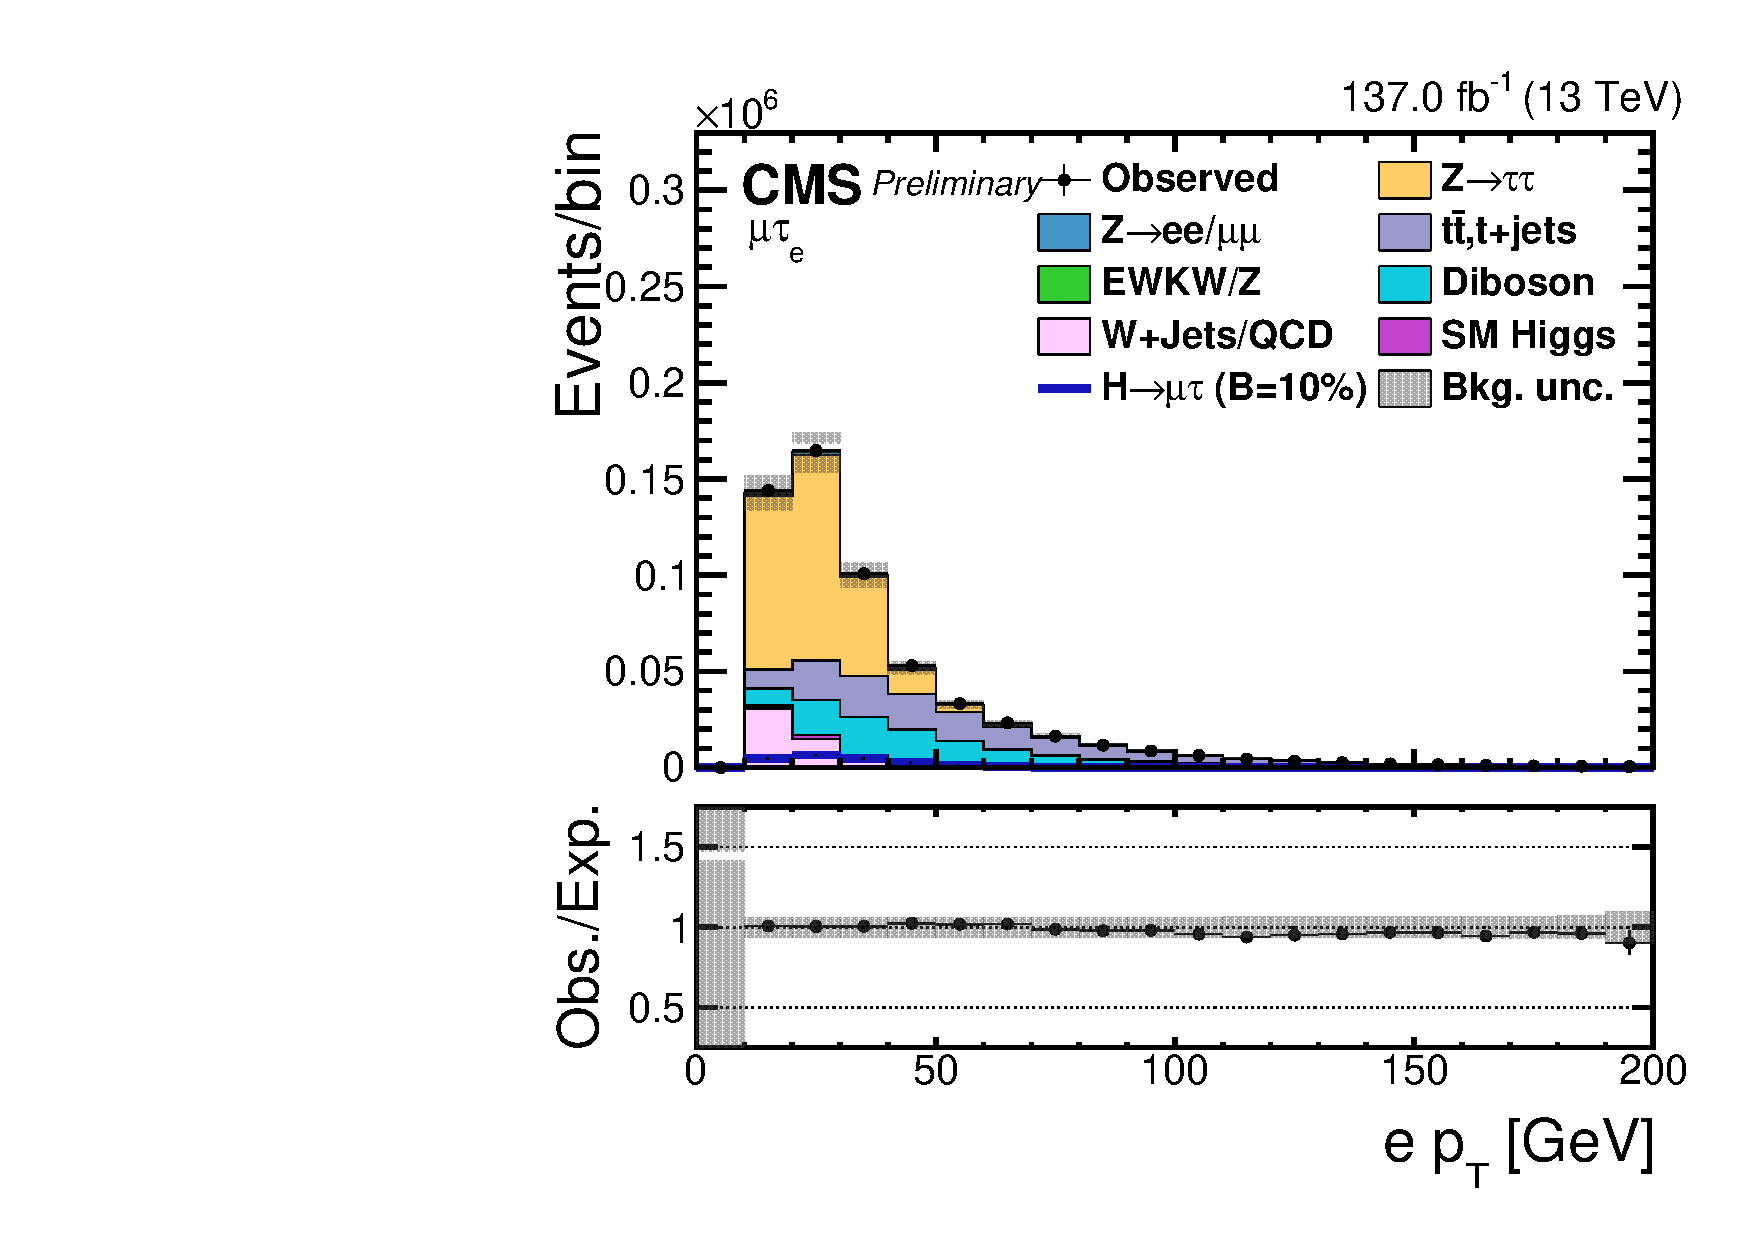
\includegraphics[width=0.36\textwidth]{plots/chapter6/mue/ePt.pdf}\\
  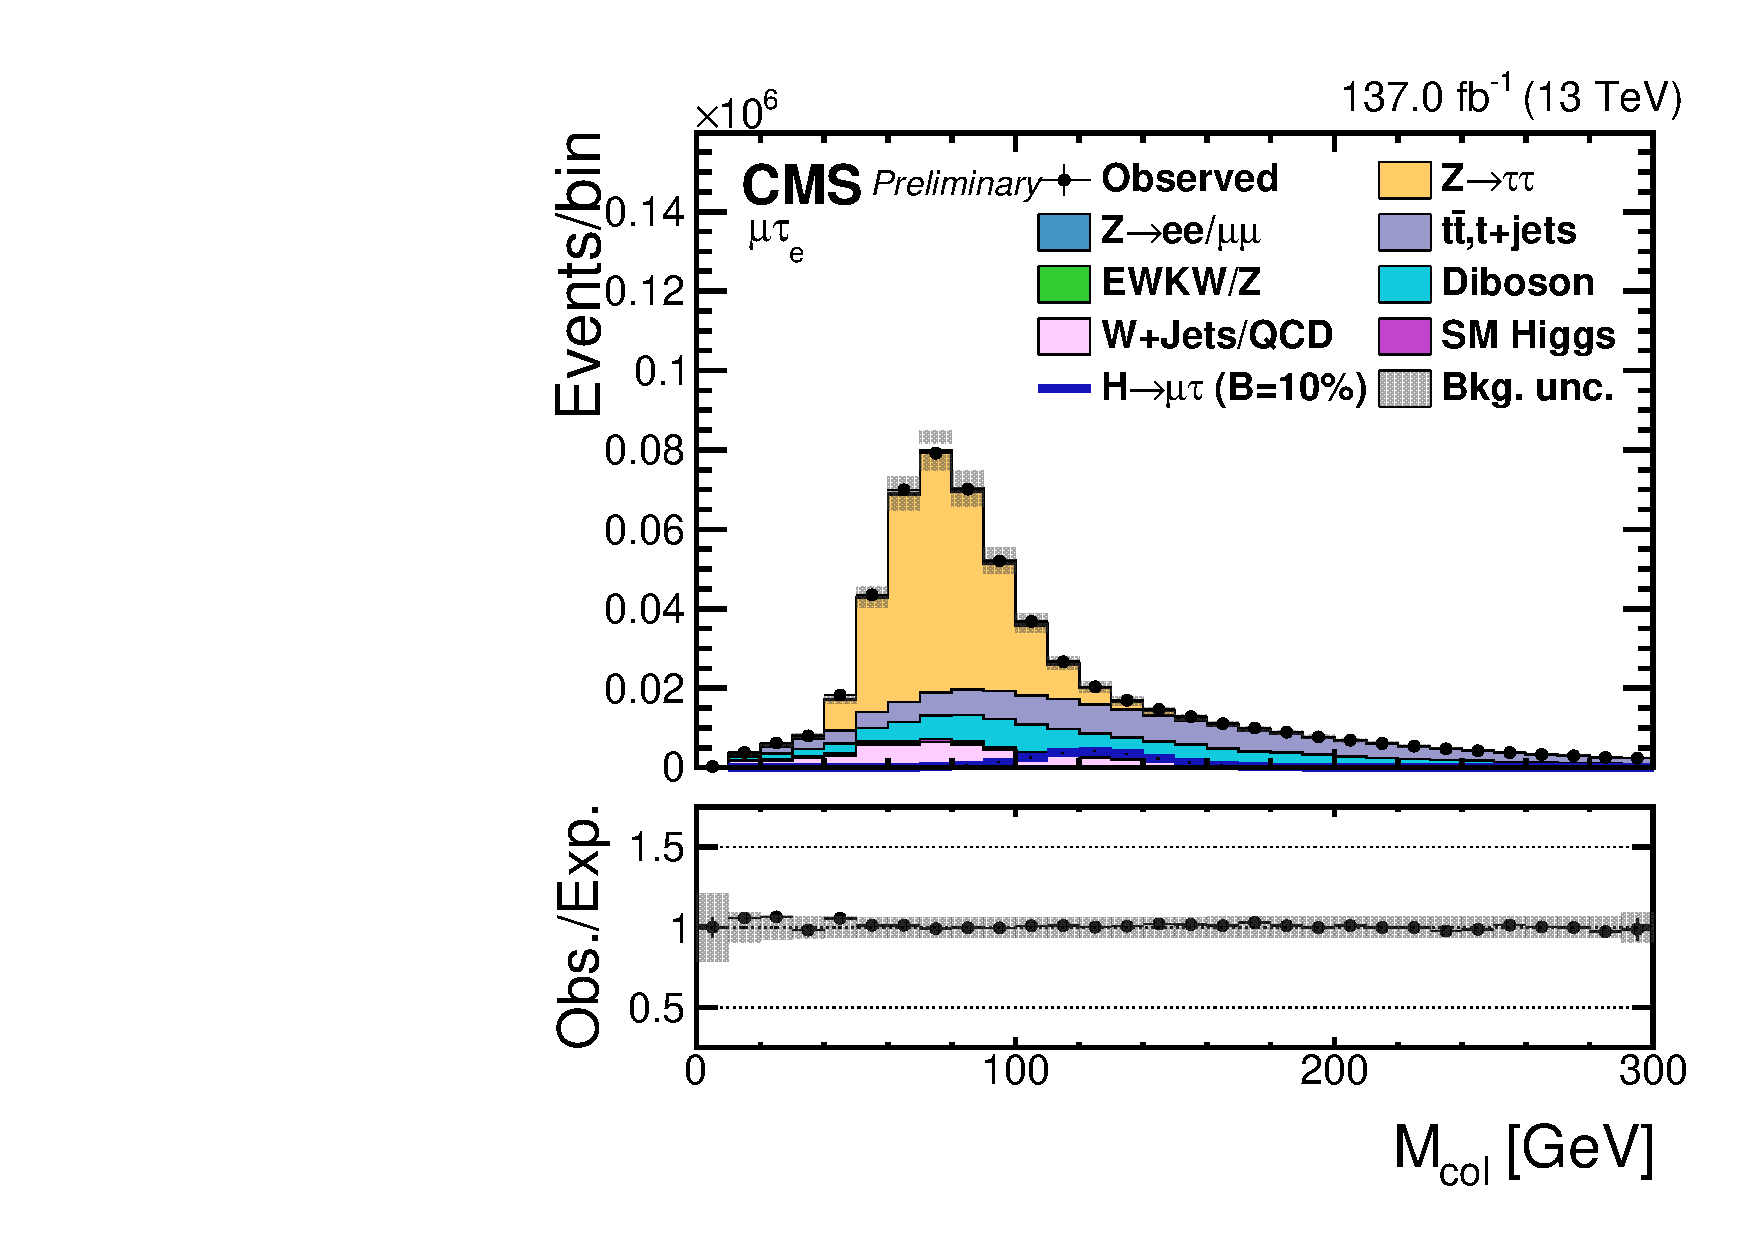
\includegraphics[width=0.36\textwidth]{plots/chapter6/mue/m_e_CollMass.pdf}
  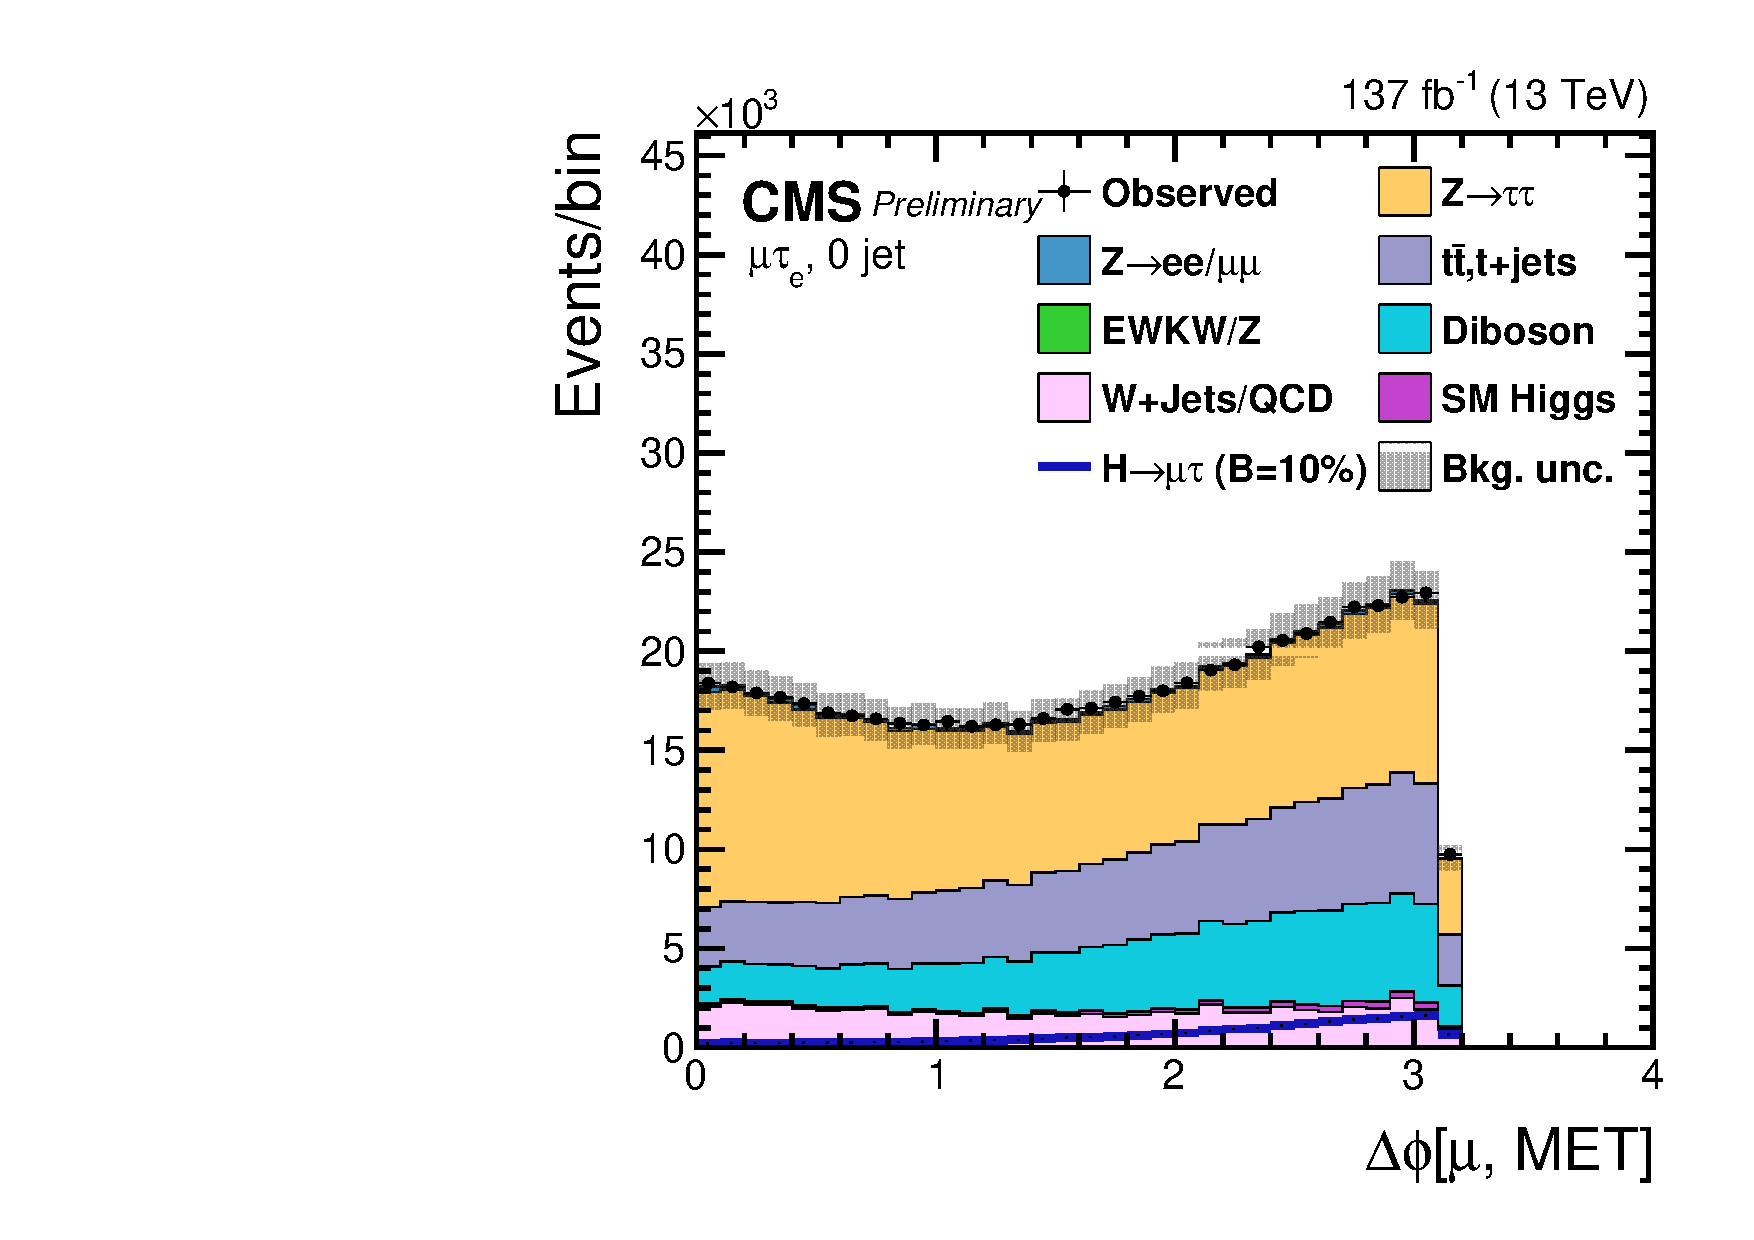
\includegraphics[width=0.36\textwidth]{plots/chapter6/mue/dPhiMuMET.pdf}\\
  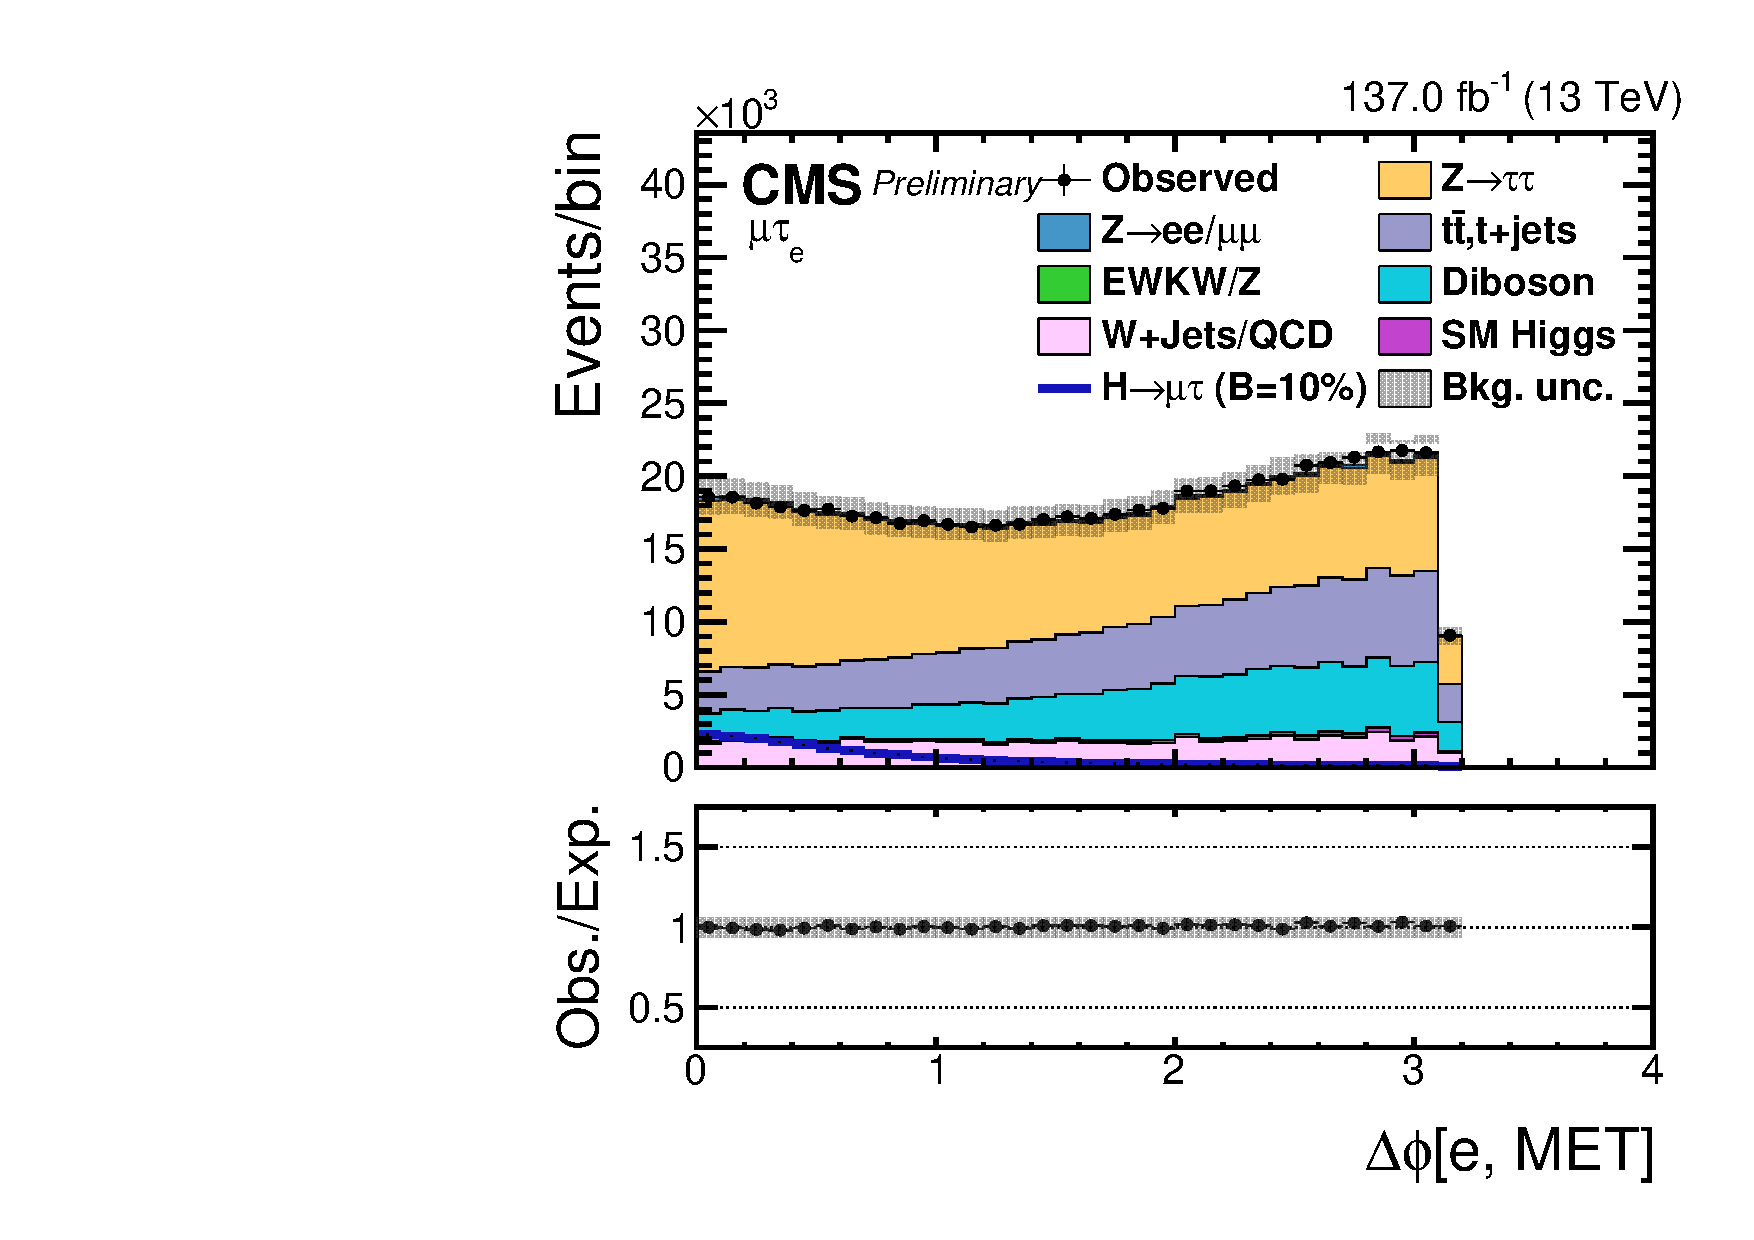
\includegraphics[width=0.36\textwidth]{plots/chapter6/mue/dPhiEMET.pdf}
  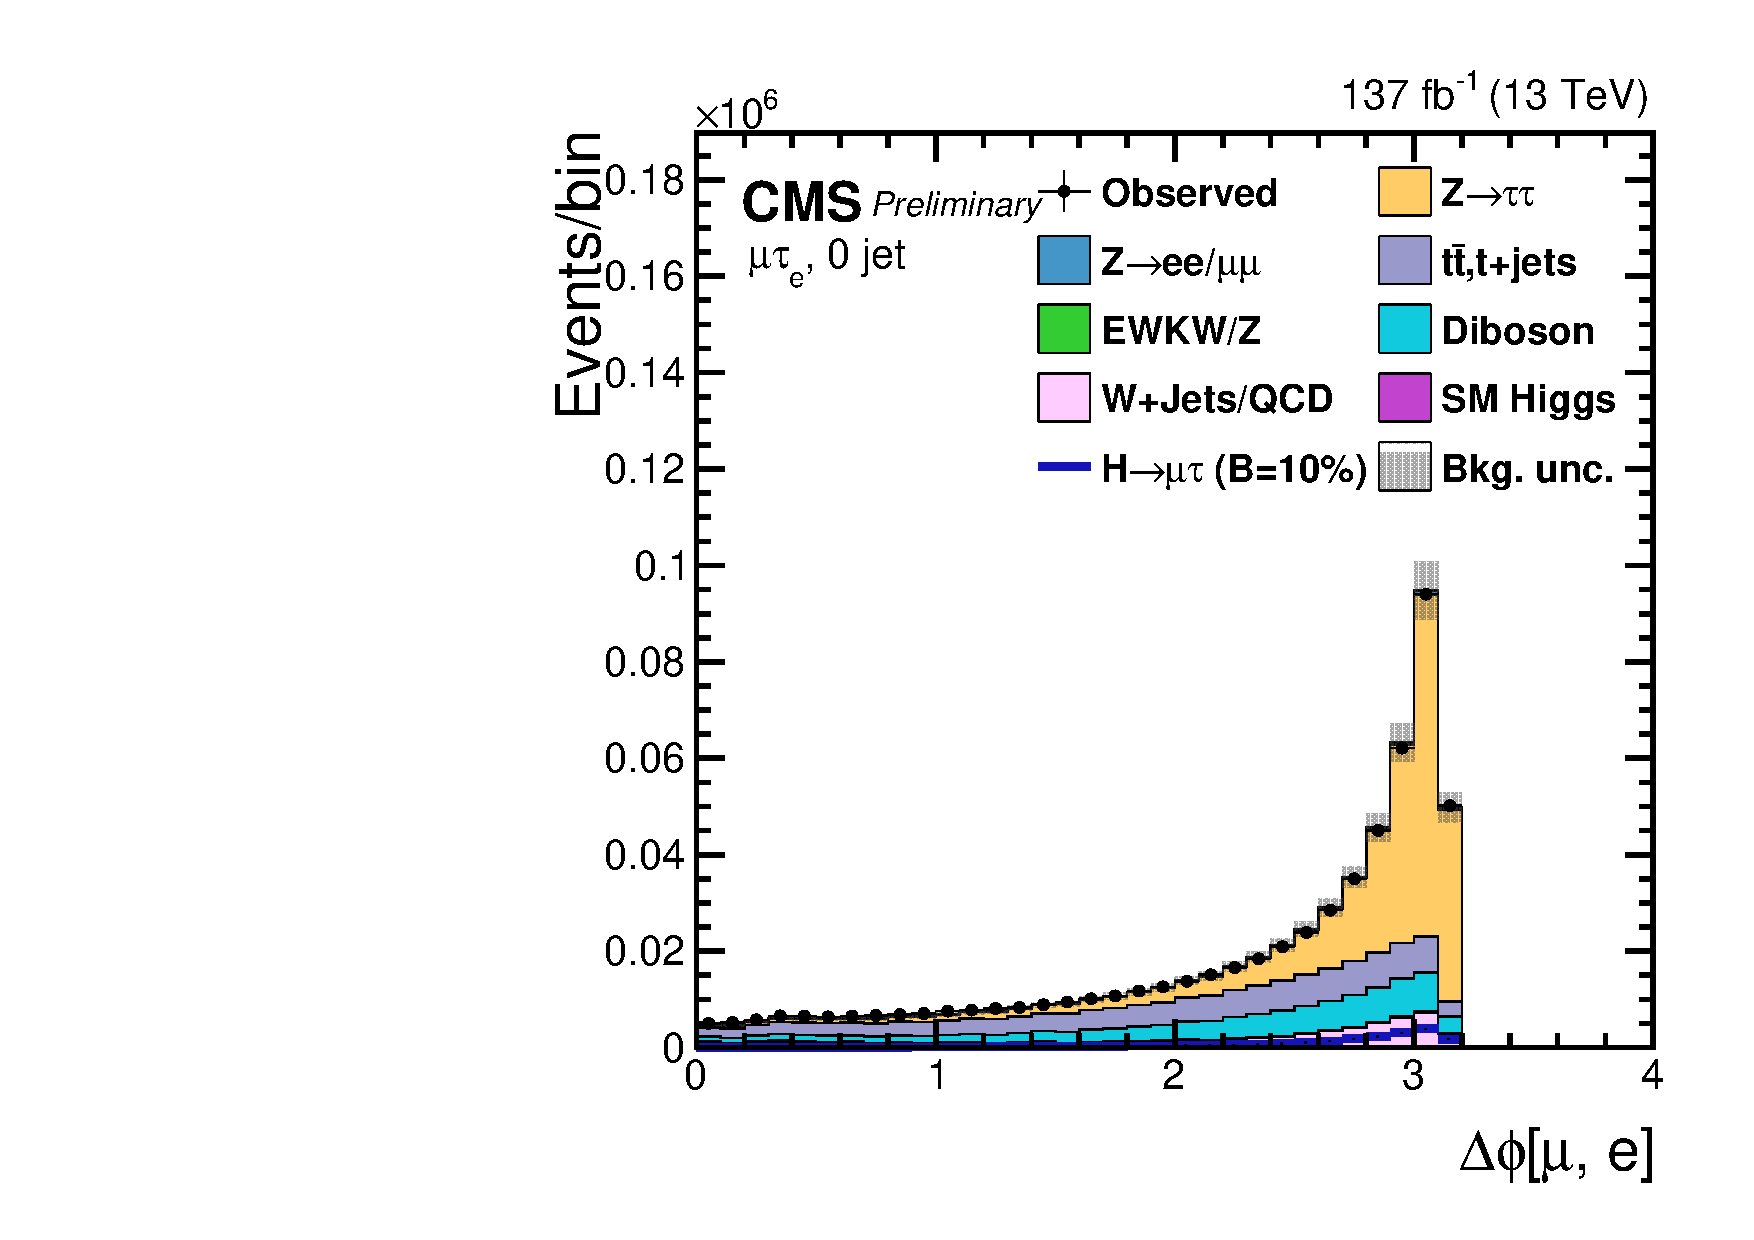
\includegraphics[width=0.36\textwidth]{plots/chapter6/mue/dPhiMuE.pdf}\\
  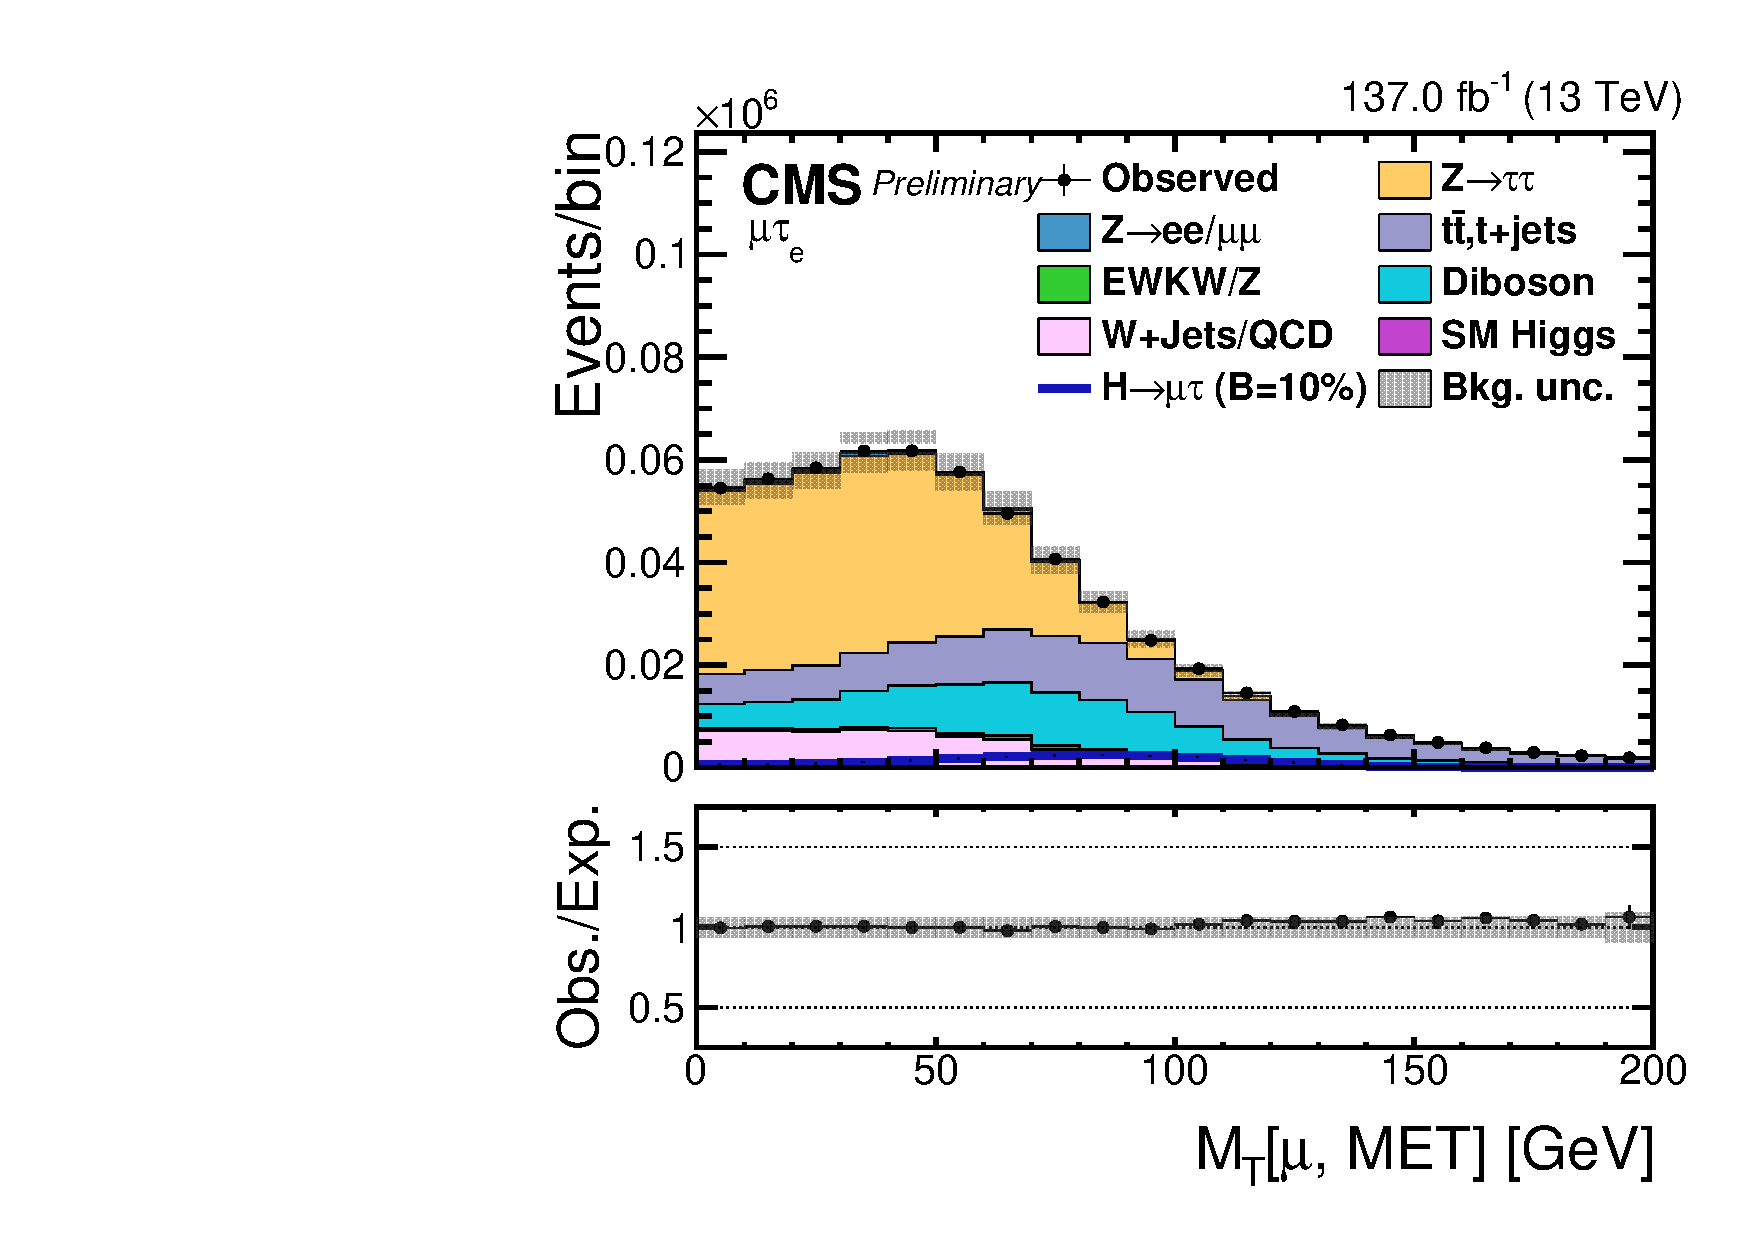
\includegraphics[width=0.36\textwidth]{plots/chapter6/mue/MTMuMET.pdf}
  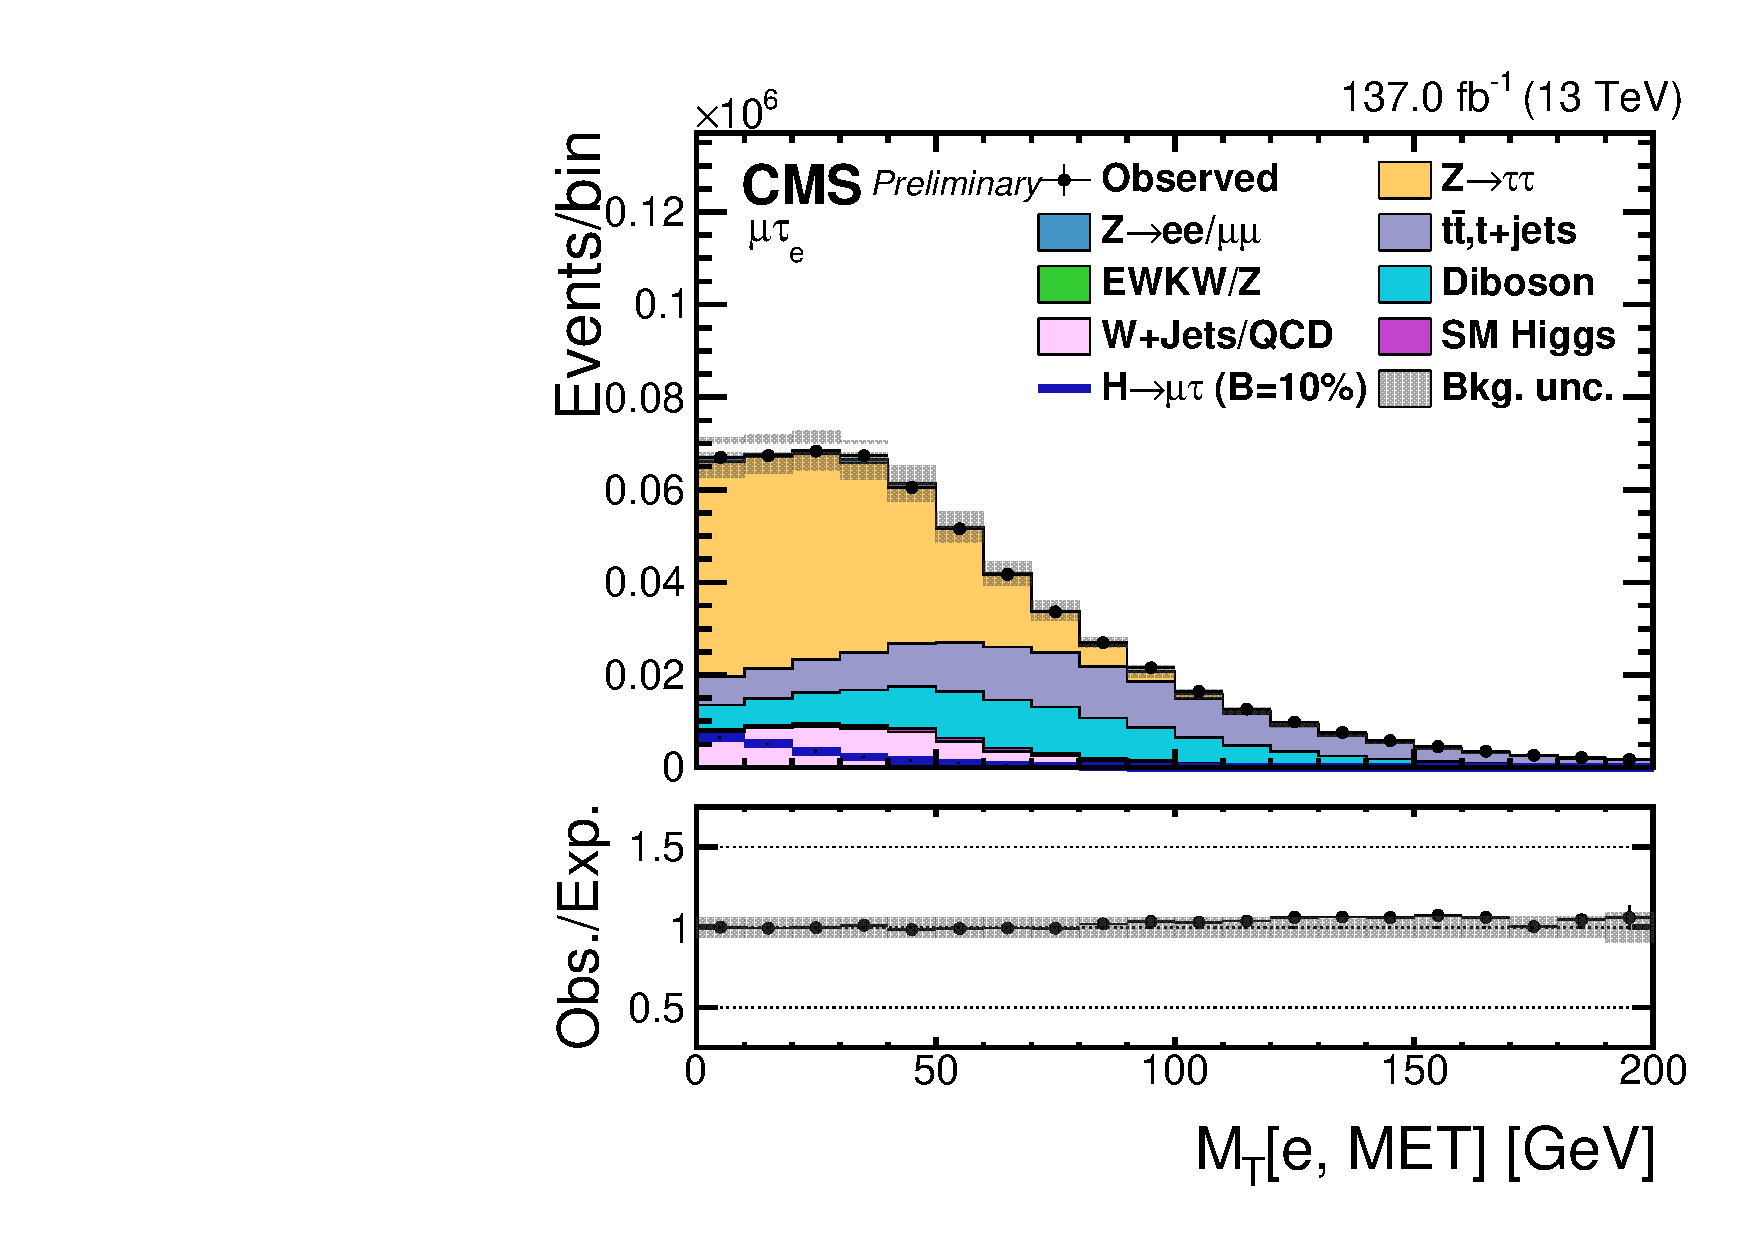
\includegraphics[width=0.36\textwidth]{plots/chapter6/mue/MTEMET.pdf}\\
  \caption{Distribution of the input variables to the BDT for the \Hmue process.}
  \label{fig:input_me}
\end{figure}

In the \mcol fit method, additional selection criteria require a stringent selection on muons, $\pt > 30\GeV$ for $0-$jet category and $\pt > 26\GeV$ in rest of the categories. The \mt(\Pgm, \ptvecmiss) is required to be greater than 60, 40, 15 and 15\GeV for $0-, 1-, 2-$jet GGF and VBF categories, respectively, while azimuthal separation between the electron and \ptvecmiss is required to be less than 0.7, 0.7, 0.5 and 0.3 for $0-, 1-, 2-$jet GGF and VBF categories, respectively. For the $0-$ and $1-$jet categories $\dphiem > 2.5$ and 1.0, respectively. The preselections and the selections for \Hmuhad and \Hmue channels in all categories are summarized in Table ~\ref{tab:mutau_evtselection}. The \mcol distributions of simulated signal, data, and backgrounds for each category in \Hmue channel, are shown in results chapter.

\begin{figure}[htbp]
  \centering
  \subfigure[]{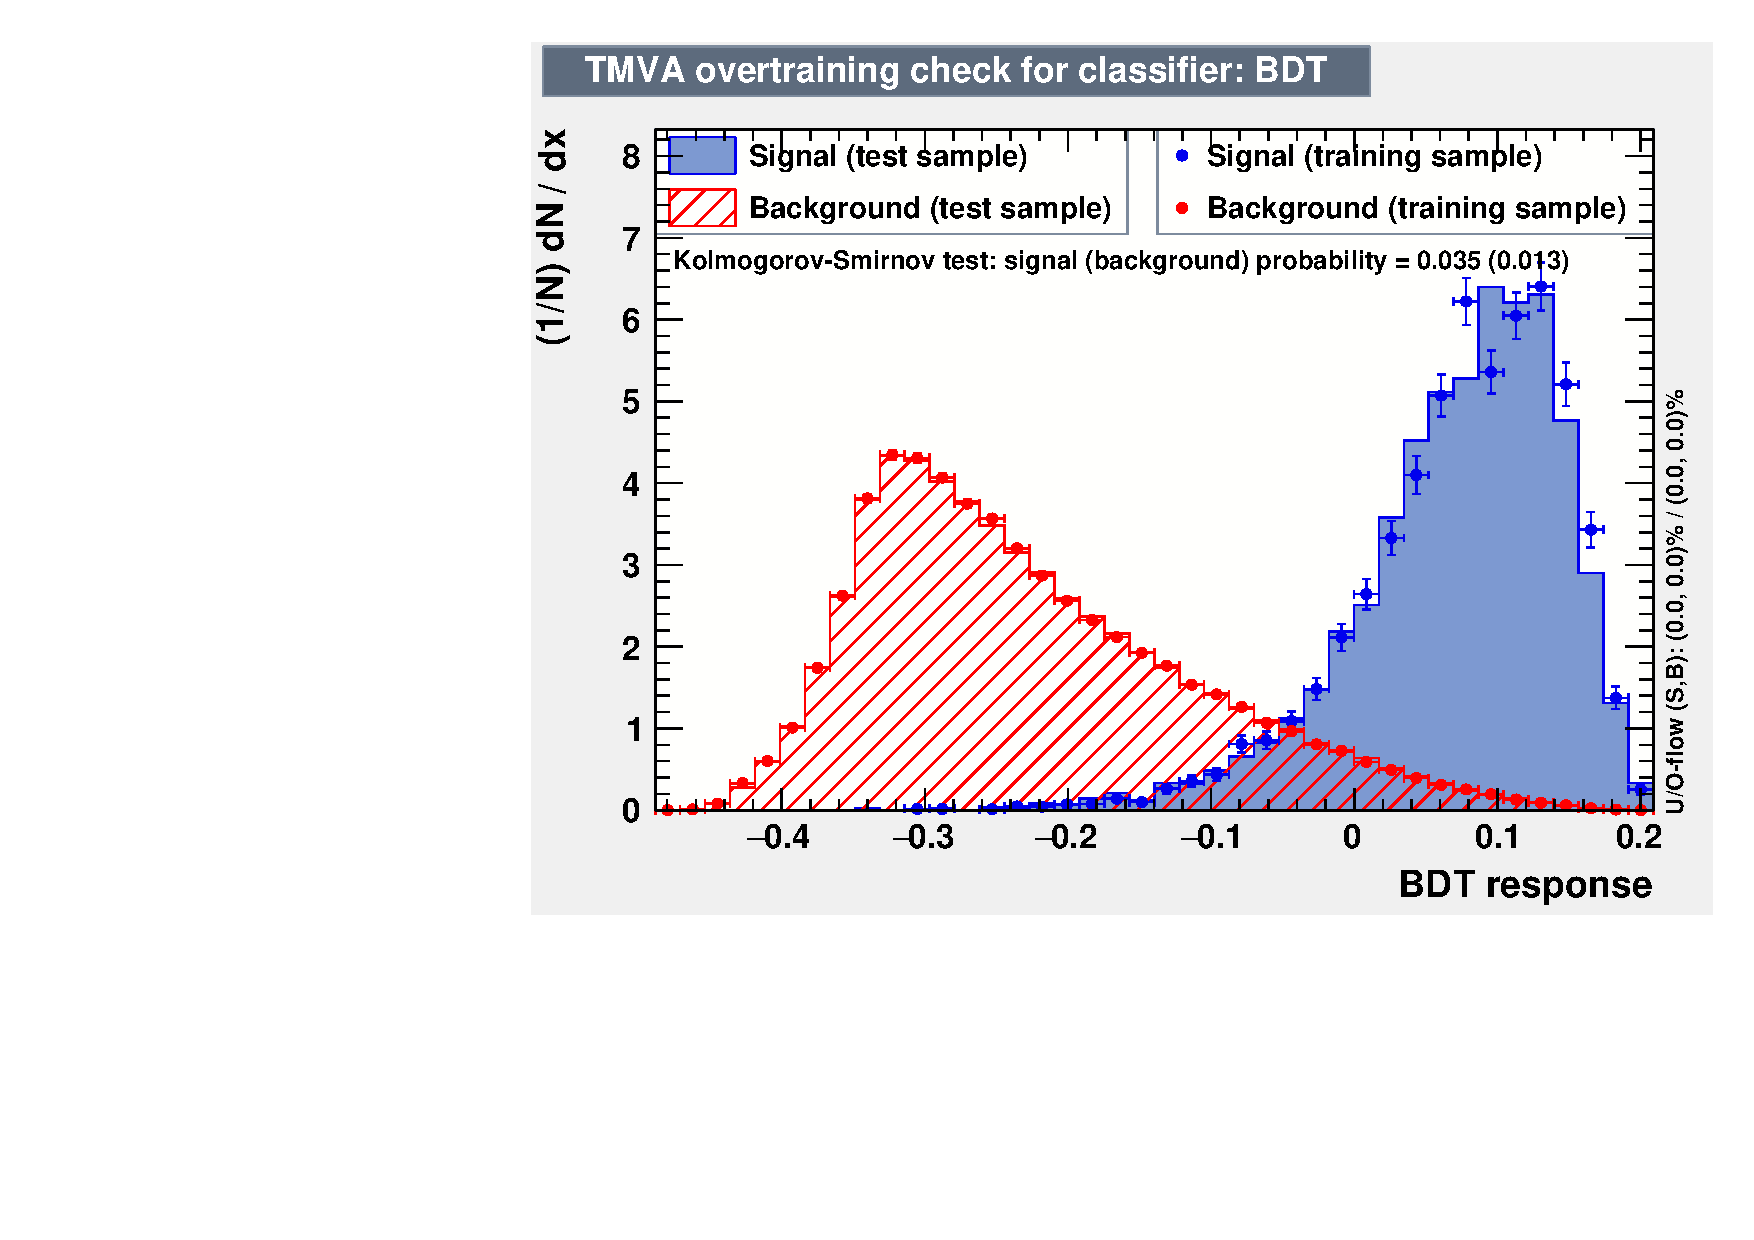
\includegraphics[width=0.32\textwidth]{plots/chapter6/BDT/mue/2016.pdf}}
  \subfigure[]{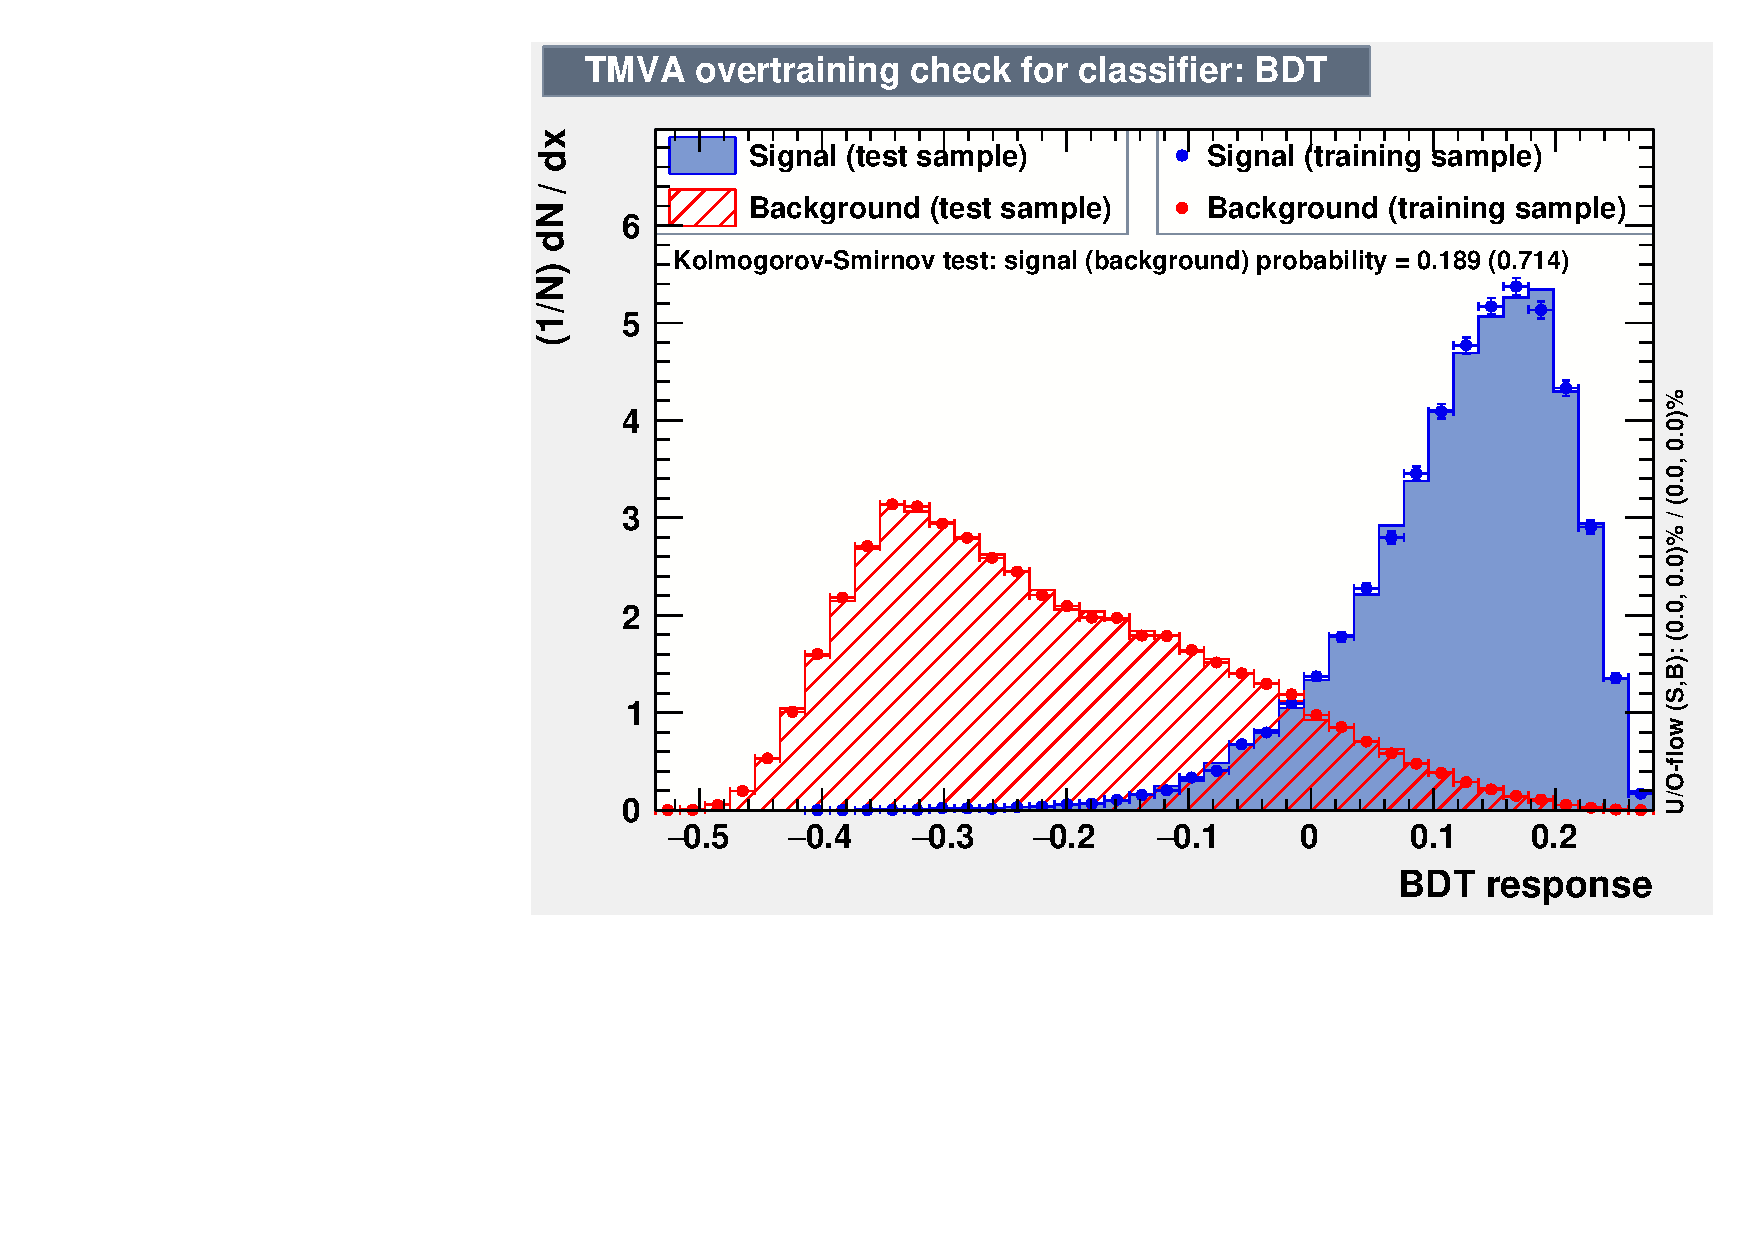
\includegraphics[width=0.32\textwidth]{plots/chapter6/BDT/mue/2017.pdf}}
  \subfigure[]{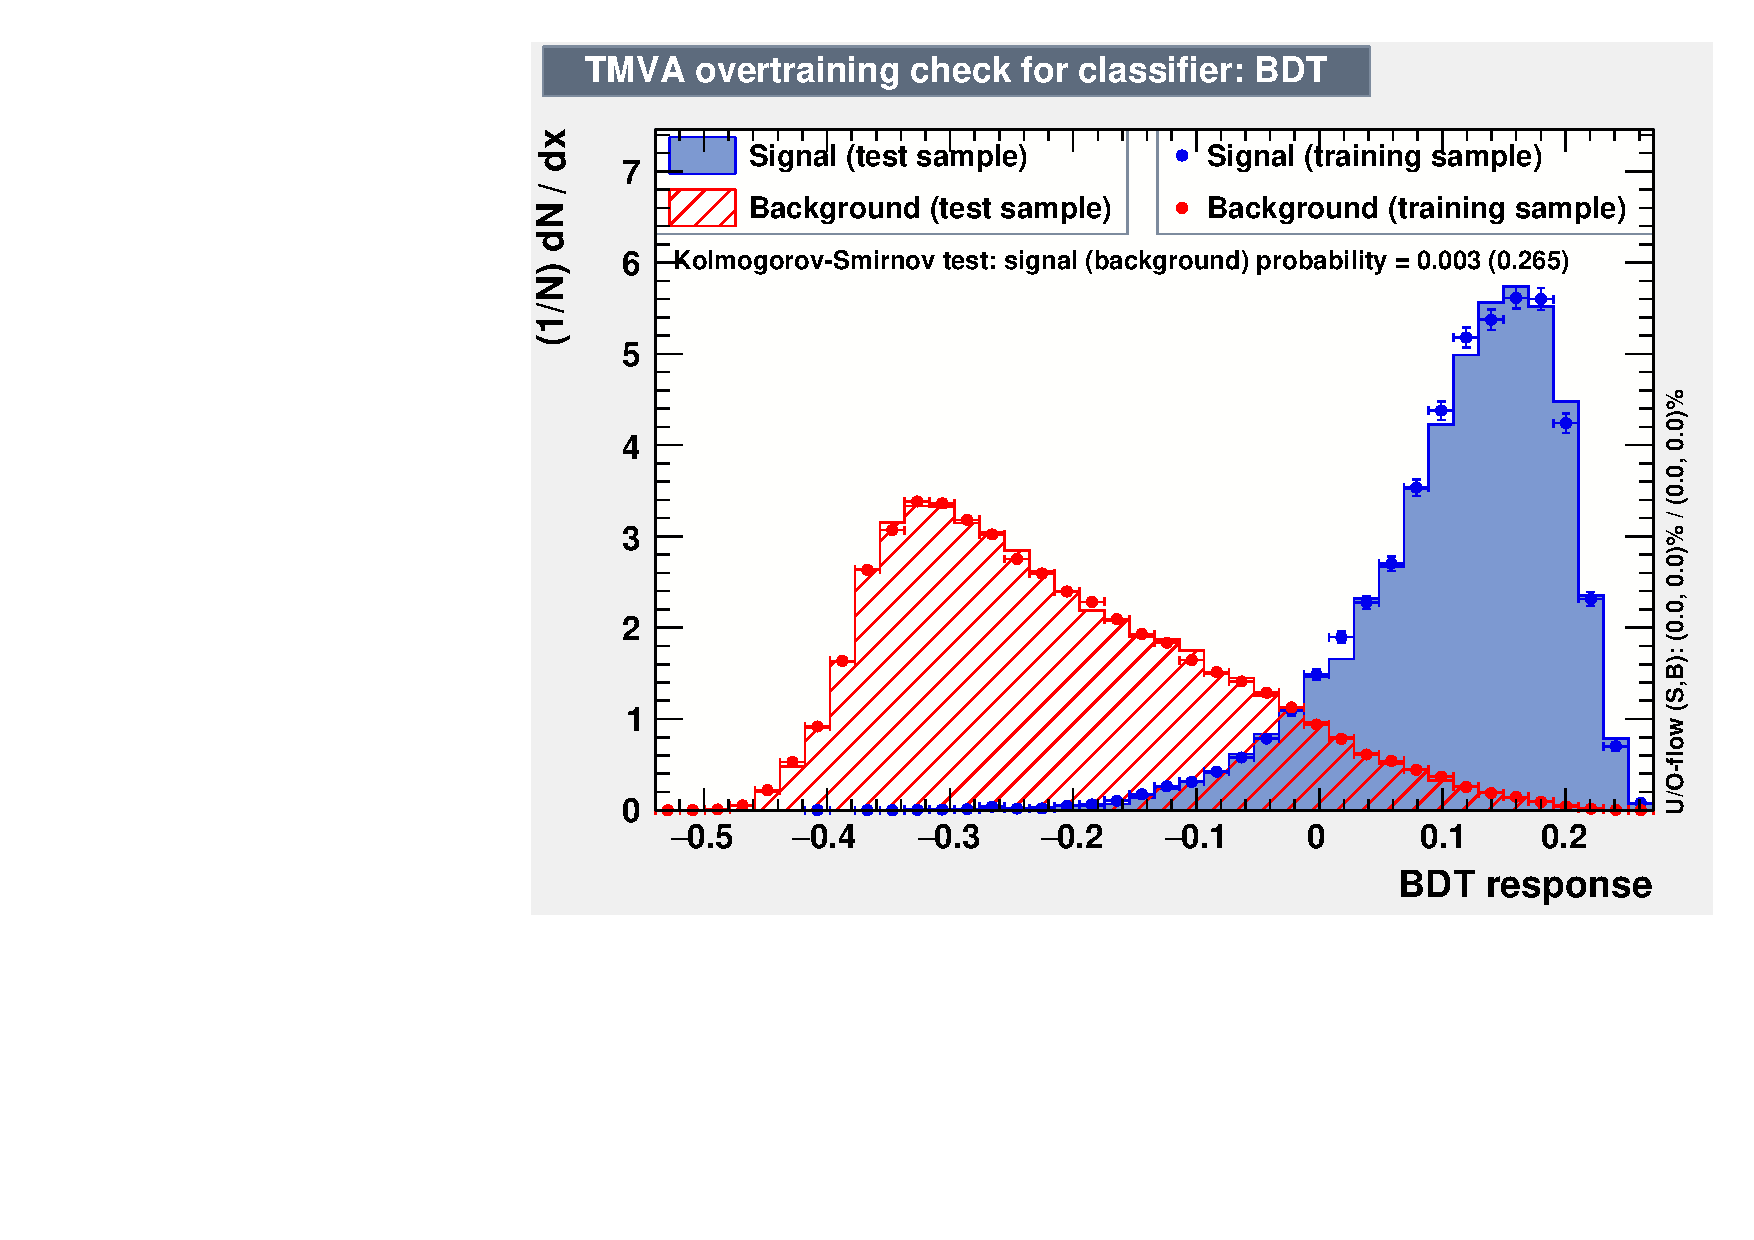
\includegraphics[width=0.32\textwidth]{plots/chapter6/BDT/mue/2018.pdf}}
  \caption{Overtraining check as performed in TMVA for the trained BDT in \Hmue channel for 2016 (a), 2017 (b), and 2018 (c).}
  \label{fig:mutaue_bdttrain}
\end{figure}

\section{\texorpdfstring{\Hehad}{Hetauh} channel}
The first step is to require the events to pass a single electron trigger. For 2016 data, this trigger has an electron \pt\, threshold of 25\GeV. However, for the 2017 and 2018 data, the trigger with the 25\GeV threshold is prescaled. Single-electron triggers with an electron \pt\, threshold of 27\GeV, 32\GeV, and 35\GeV are used in conjunction with the cross-trigger with an electron \pt\, threshold of 24\GeV and tau \pt\, threshold of 30\GeV. In addition to the event passing the trigger, the reconstructed leptons corresponding to the trigger have to match the HLT objects within $\Delta R < 0.5$.

The  preselection in this channel requires an isolated electron and an isolated \tauh candidates of opposite charge and separated by $\Delta\text{R} > 0.5$. The electron candidate is required to have $\pt > 27\GeV$, $\abs{\eta} < 2.1$ and isolation $I^{\Pgm}_\text{rel} < 0.15$. The \tauh candidate is required to have $\pt > 30\GeV$ and $\abs{\eta} < 2.3$. Events containing additional electrons, muons, or \tauh candidates or at least one b jet tagged by DeepCSV algorithm are removed.

A BDT is trained after applying preselection criteria. The same training samples, as used in the \Hmuhad channel, are considered. The list of input variables to BDT training stays the same, except for the addition of the visible mass, \mvis variable, and removal of \ptvecmiss. The \mvis variable is more useful as the relative composition of the two channels' backgrounds is different. In particular, $\Zee+$jets background contributes more with respect to $\Zmm+$jets background. The distribution of the input variables to the BDT can be seen in Figure ~\ref{fig:input_et}. The BDT discriminator distributions of simulated signal, data, and backgrounds for each category in \Hehad channel, are shown in results chapter.

\begin{figure}[htbp!]
  \centering
  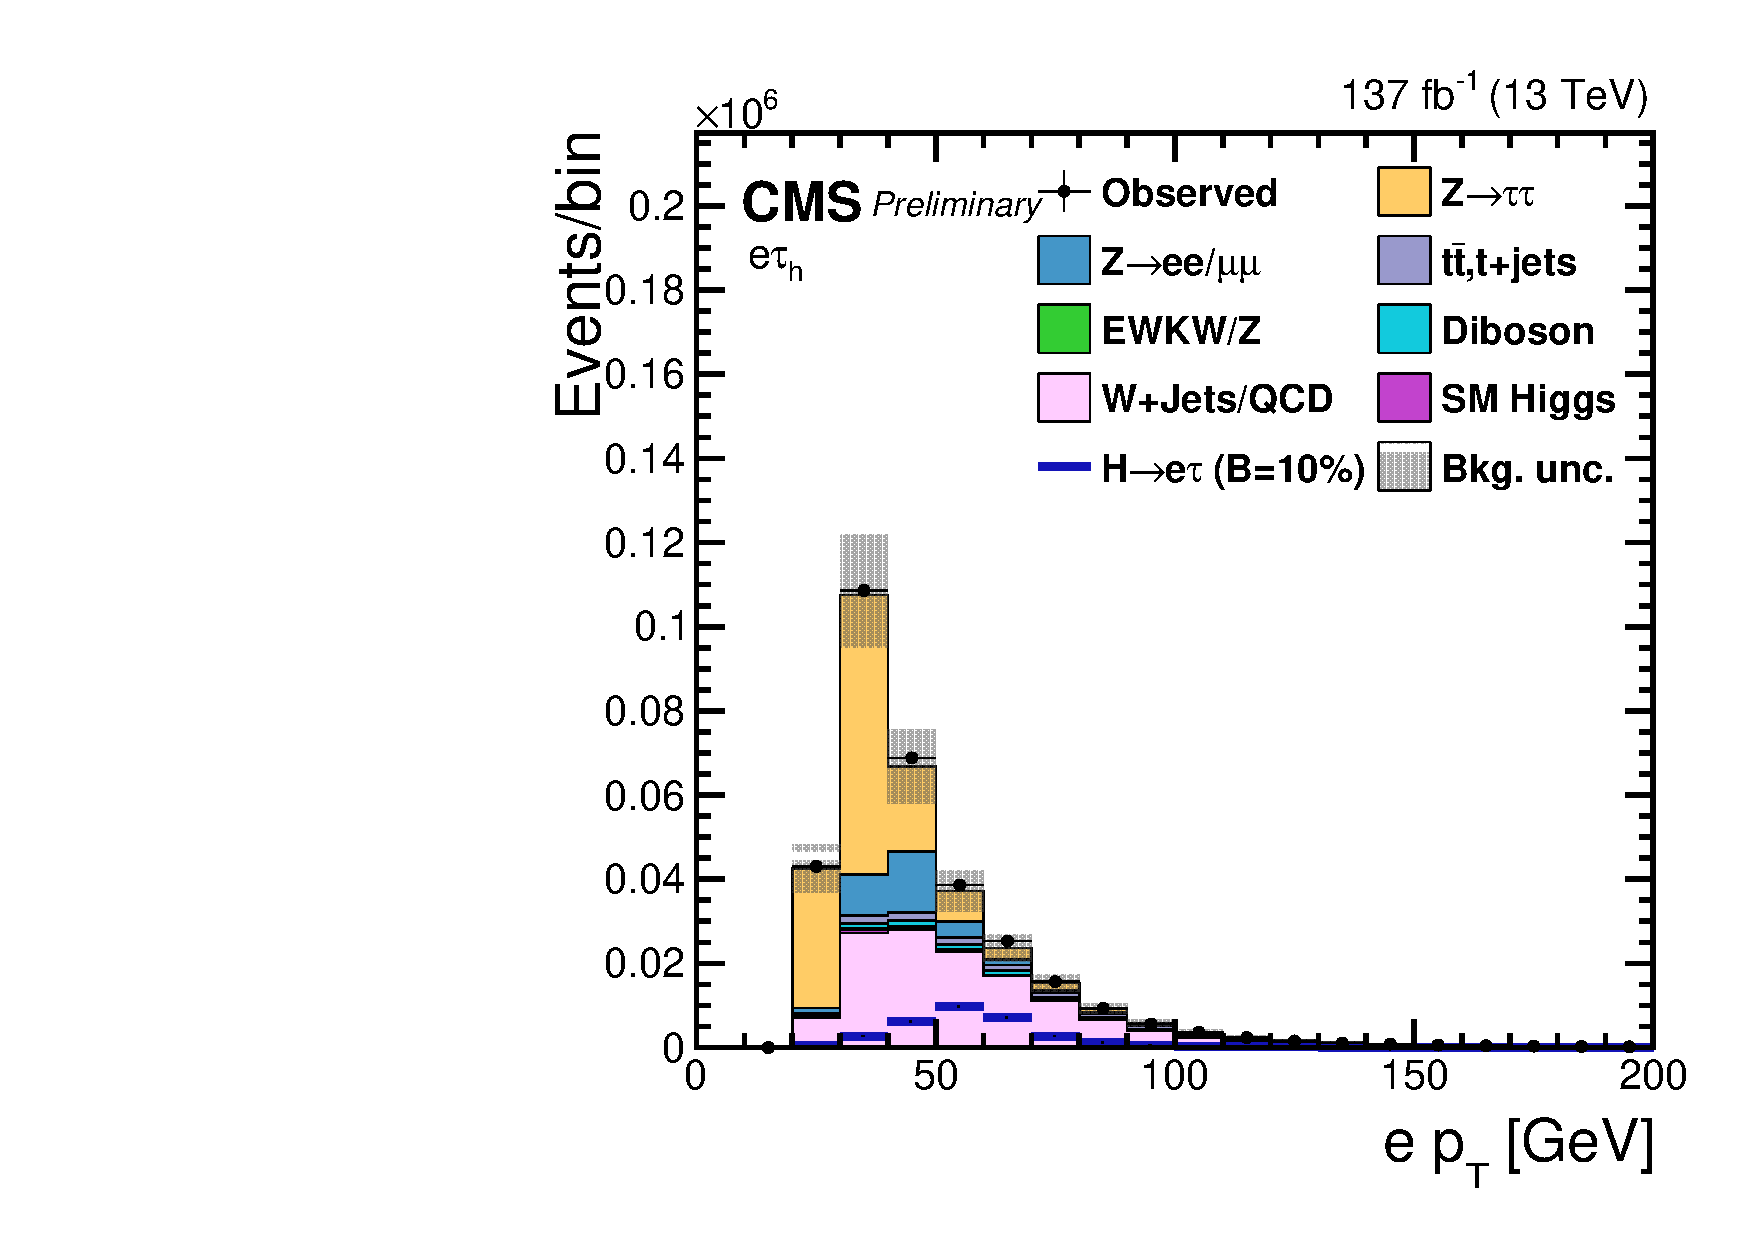
\includegraphics[width=0.36\textwidth]{plots/chapter6/etau/ePt.pdf}
  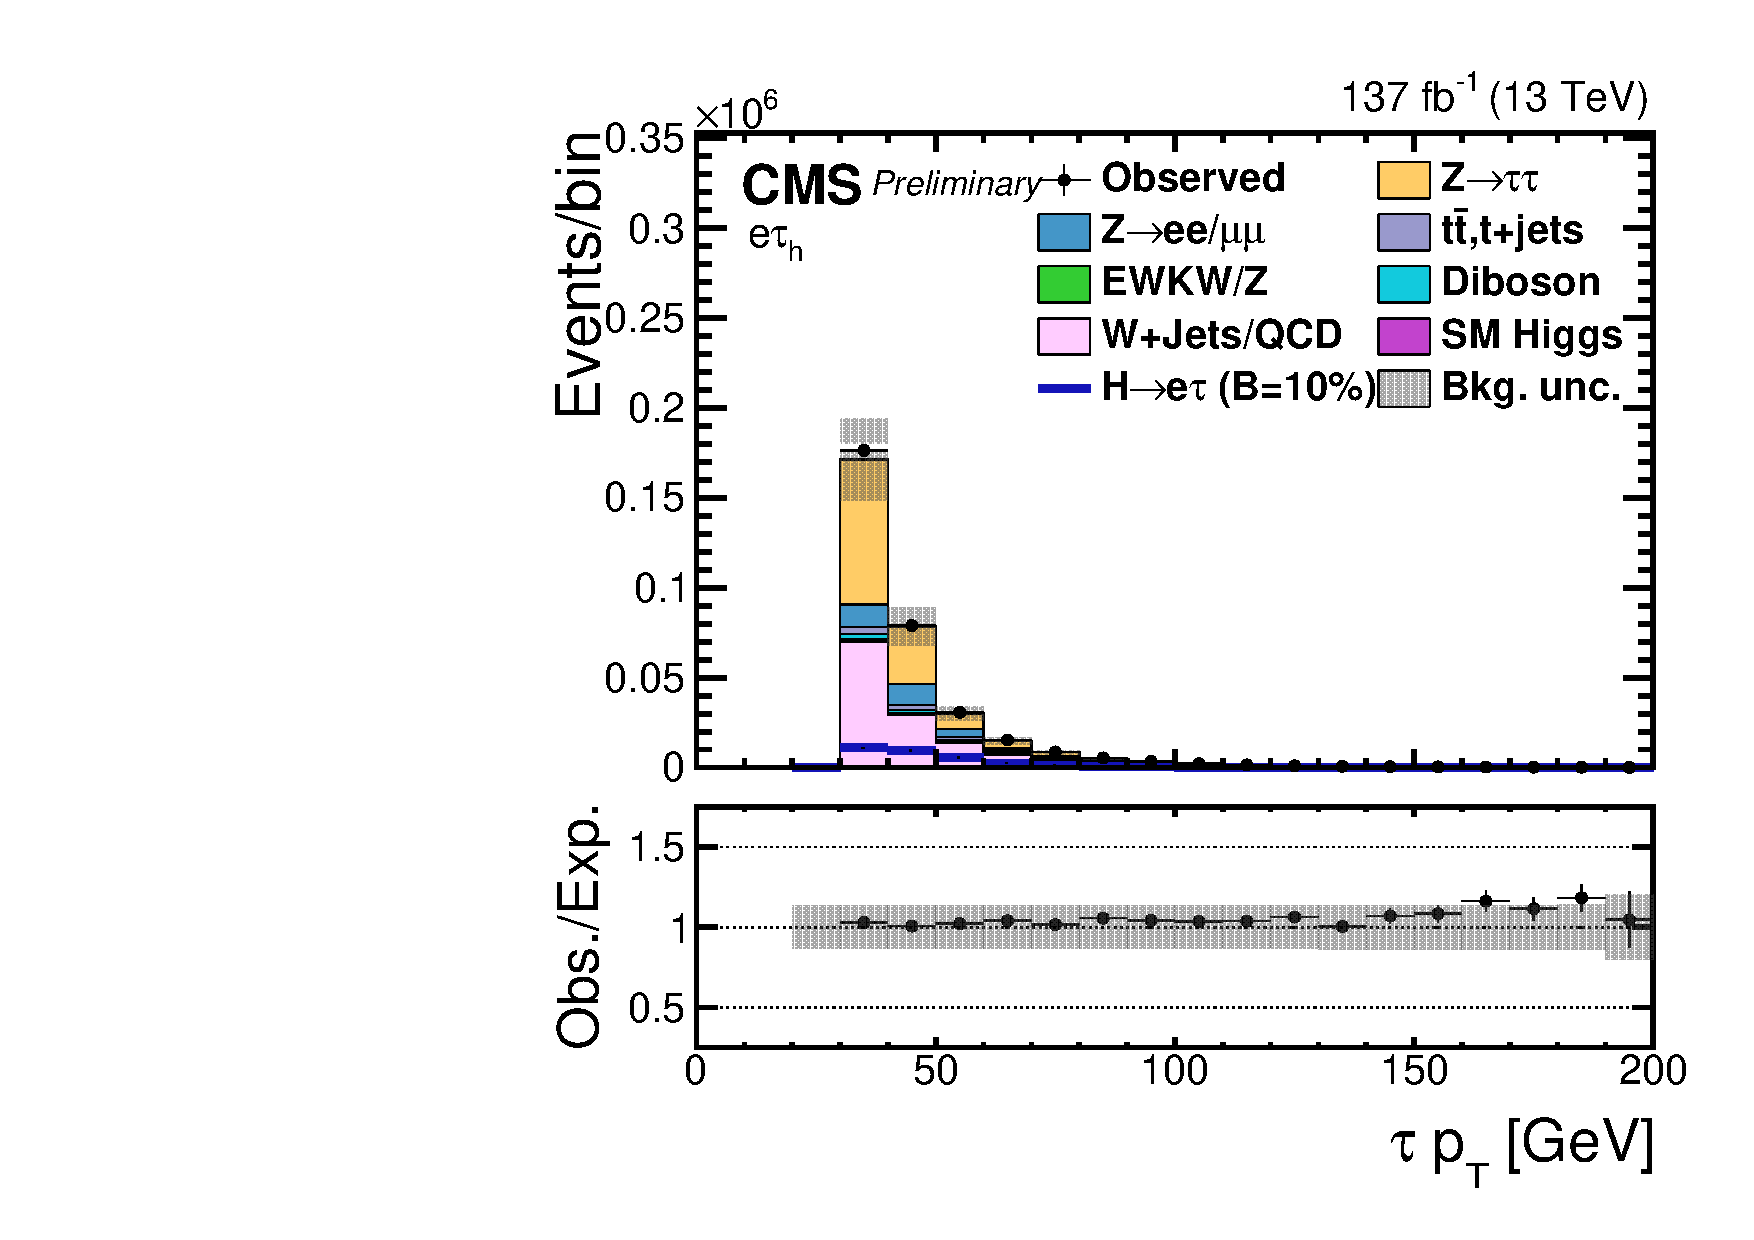
\includegraphics[width=0.36\textwidth]{plots/chapter6/etau/tPt.pdf}\\
  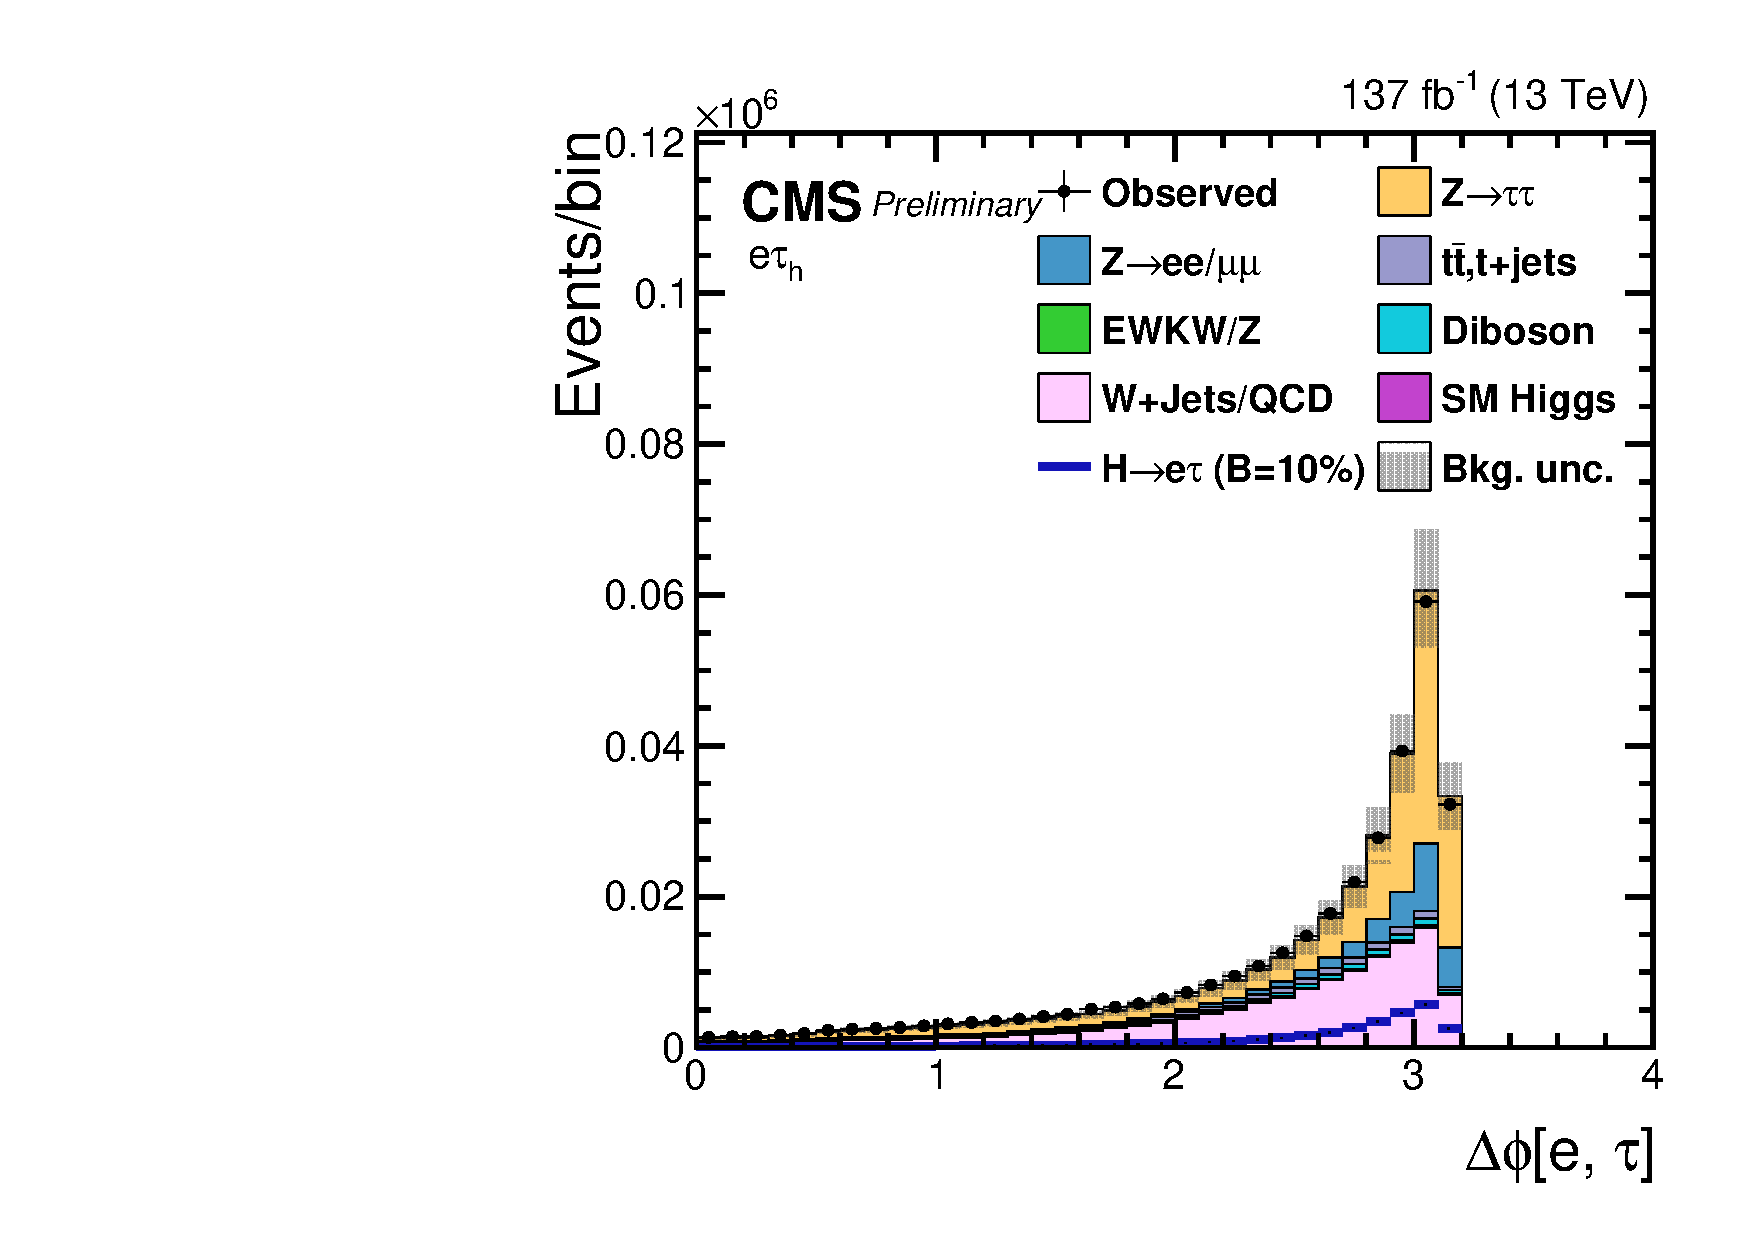
\includegraphics[width=0.36\textwidth]{plots/chapter6/etau/dPhiETau.pdf}
  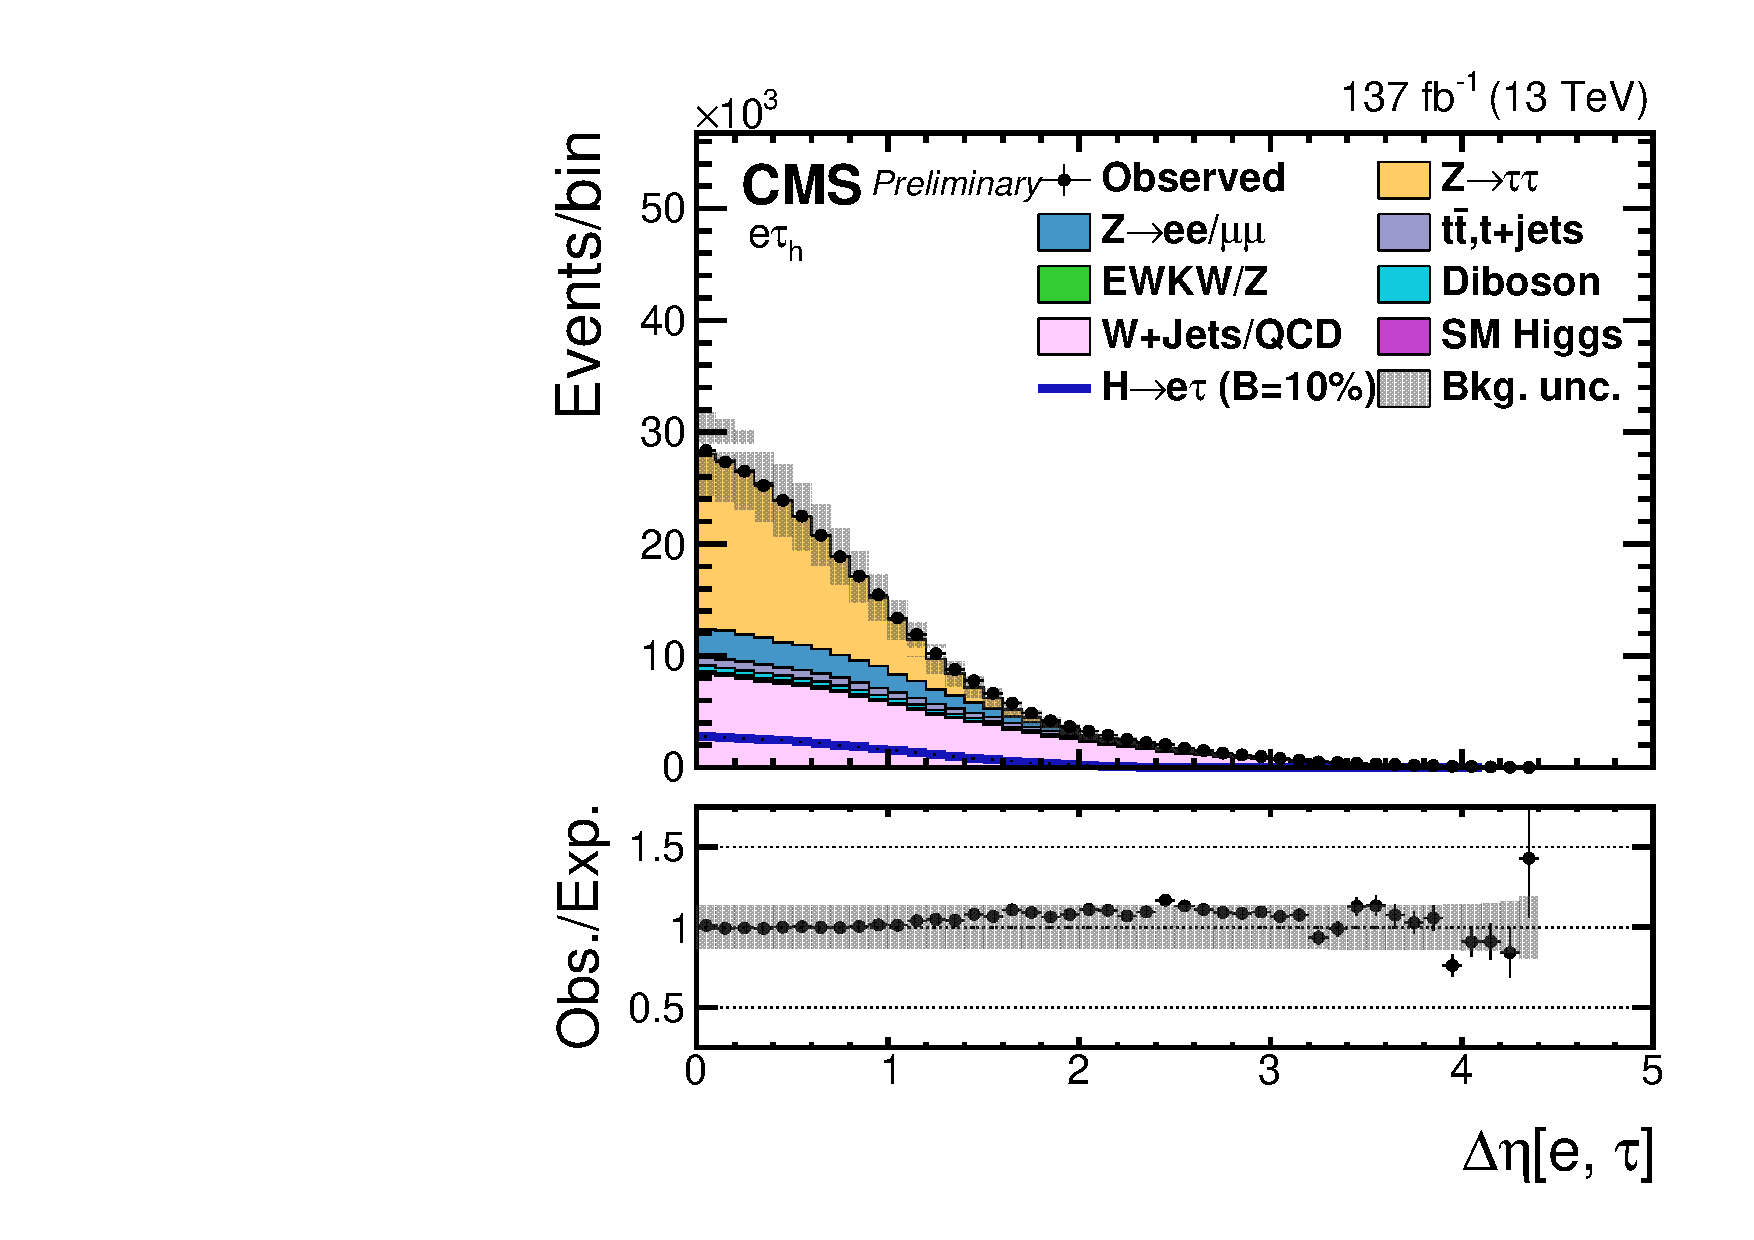
\includegraphics[width=0.36\textwidth]{plots/chapter6/etau/dEtaETau.pdf}\\
  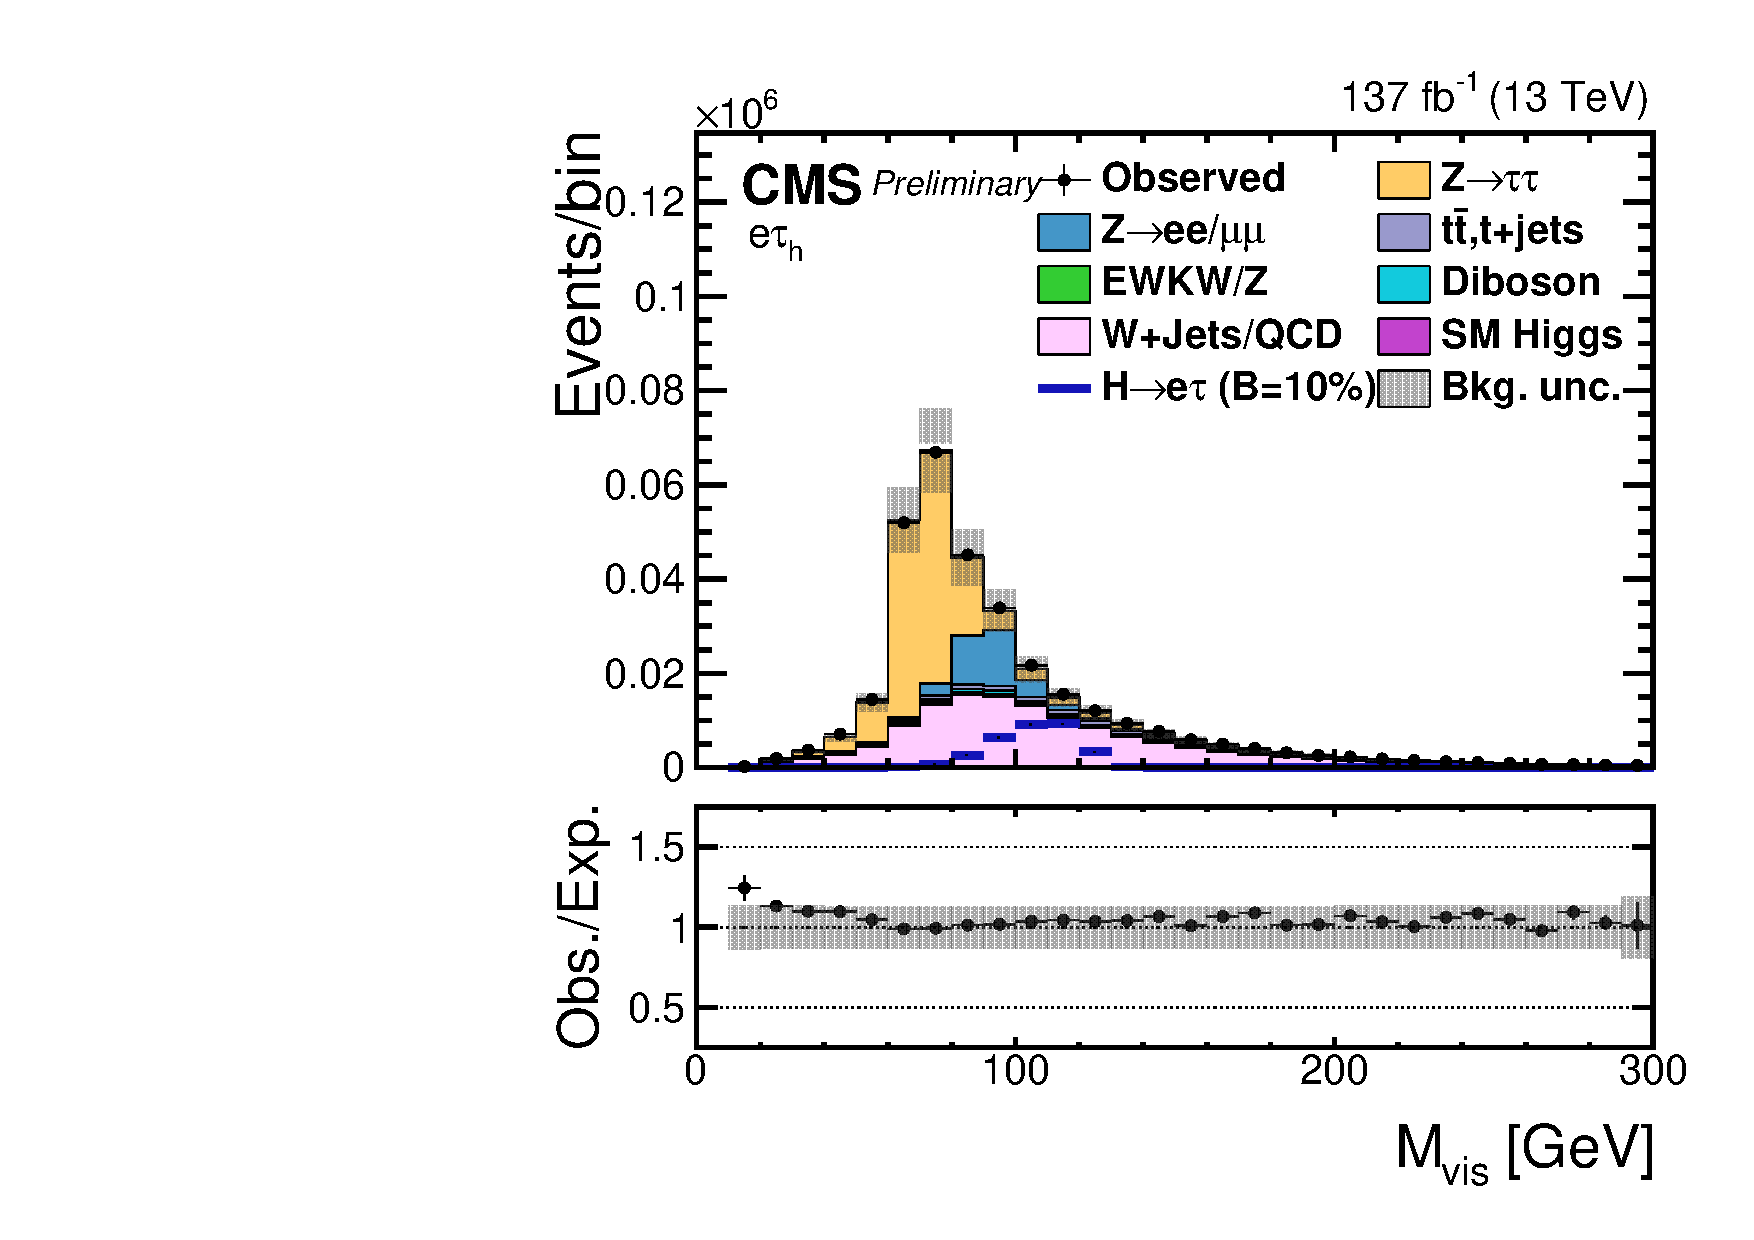
\includegraphics[width=0.36\textwidth]{plots/chapter6/etau/e_t_Mass.pdf}
  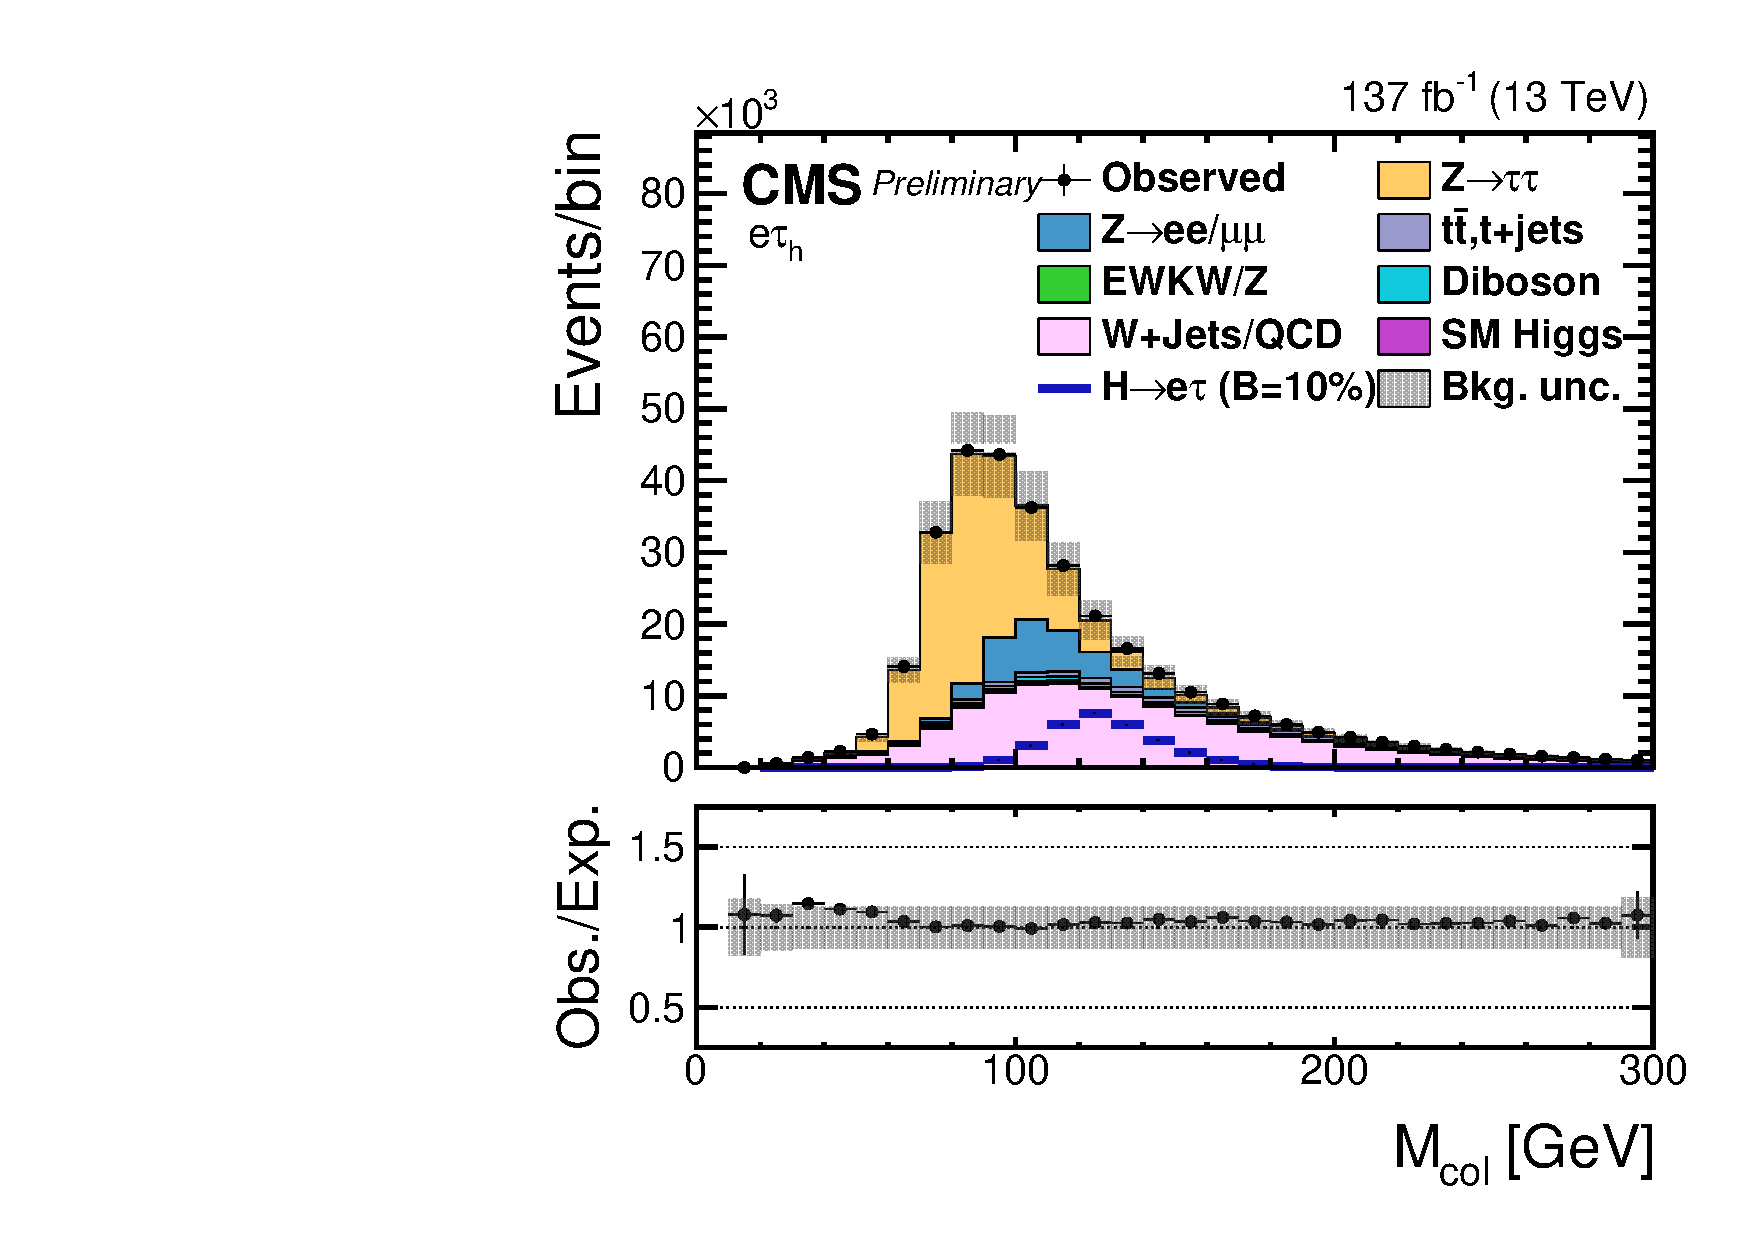
\includegraphics[width=0.36\textwidth]{plots/chapter6/etau/e_t_CollinearMass.pdf}\\
  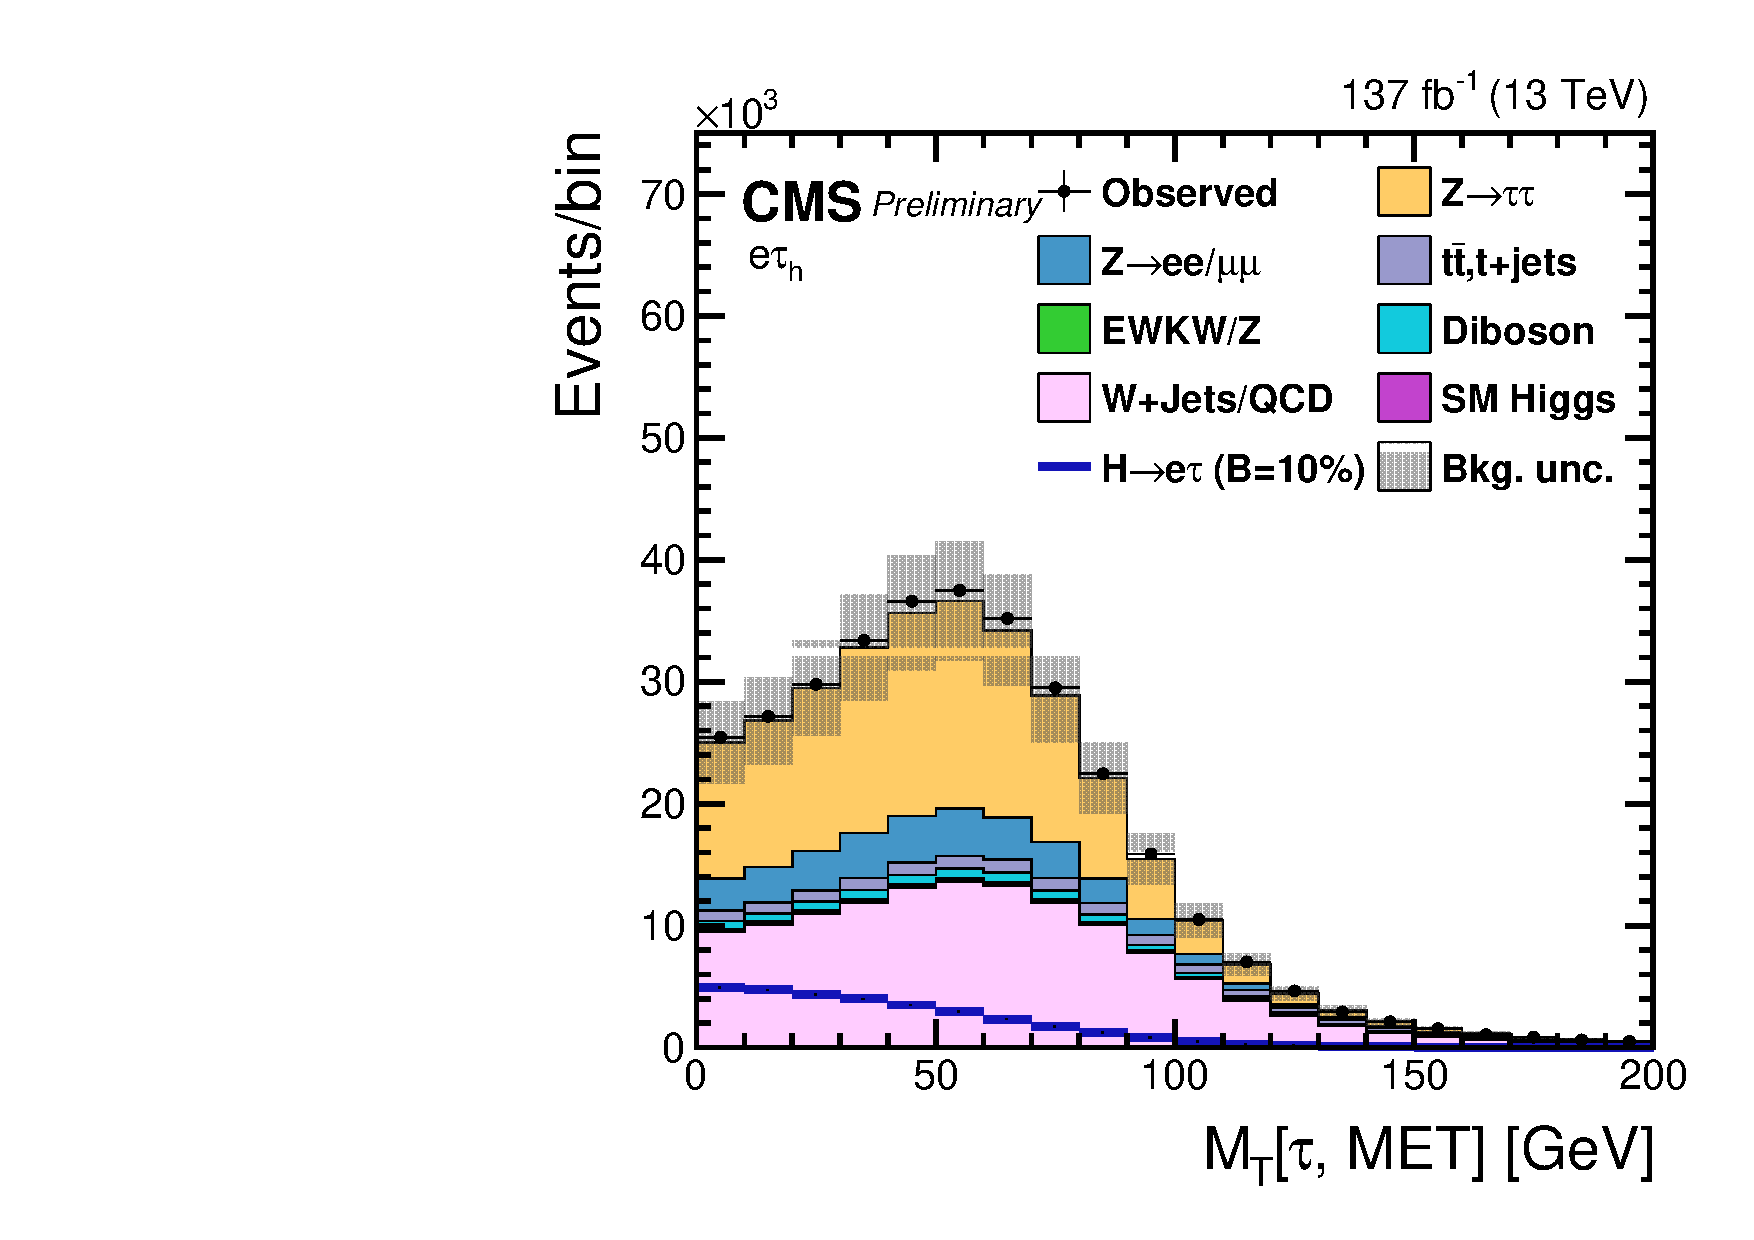
\includegraphics[width=0.36\textwidth]{plots/chapter6/etau/MTTauMET.pdf}
  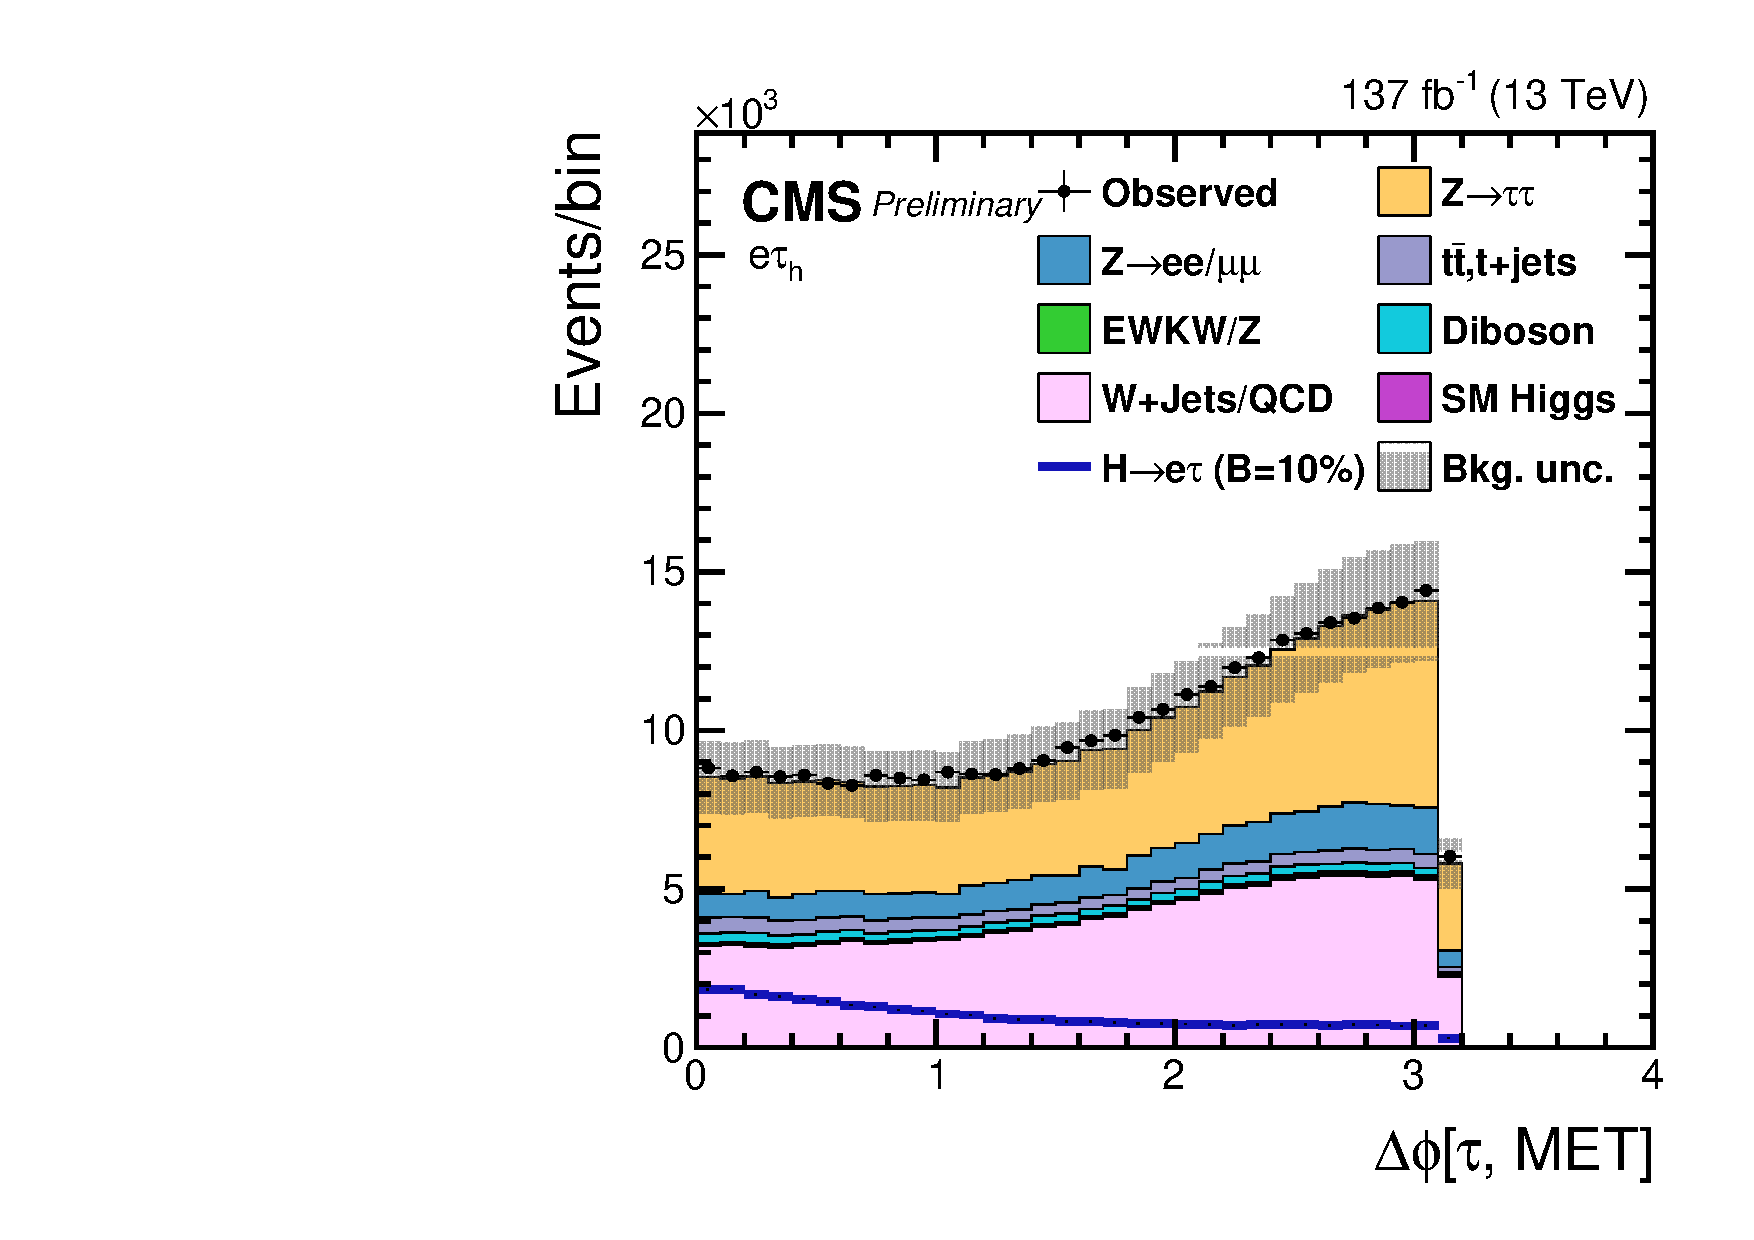
\includegraphics[width=0.36\textwidth]{plots/chapter6/etau/dPhiTauMET.pdf}\\
  \caption{Distribution of the input variables to the BDT for the \Hehad process.}
  \label{fig:input_et}
\end{figure}

In the \mcol fit method, additional selection criteria require $\mt(\tauh, \ptvecmiss) < 60\GeV$ in all the categories. The \mcol distributions of simulated signal, data, and backgrounds for each category in \Hehad channel, are shown in results chapter.

\begin{figure}[htbp]
  \centering
  \subfigure[]{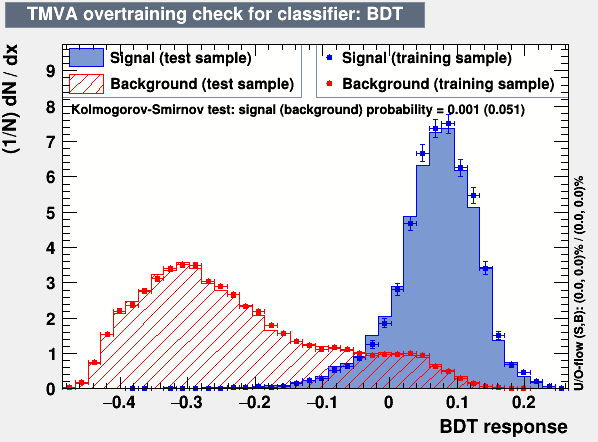
\includegraphics[width=0.32\textwidth]{plots/chapter6/BDT/etau/2016.png}}
  \subfigure[]{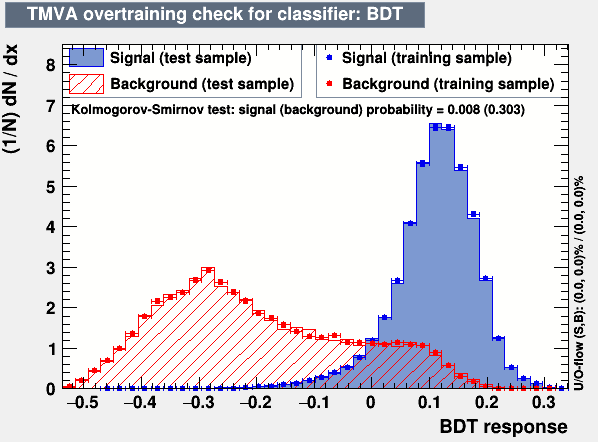
\includegraphics[width=0.32\textwidth]{plots/chapter6/BDT/etau/2017.png}}
  \subfigure[]{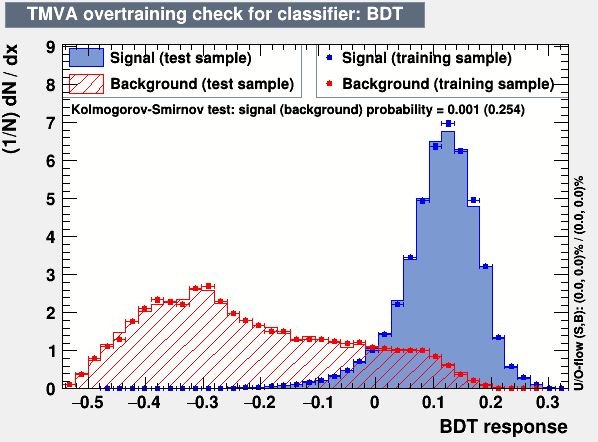
\includegraphics[width=0.32\textwidth]{plots/chapter6/BDT/etau/2018.png}}
  \caption{Overtraining check as performed in TMVA for the trained BDT in \Hehad channel for 2016 (a), 2017 (b), and 2018 (c).}
  \label{fig:etauh_bdttrain}
\end{figure}

%%% E-TAU event selection
\begin{table}[!hbpt]
\centering
\caption{Event selection criteria for the kinematic variables for the \Het channels}
\begin{tabular}{lccccccccc}
\hline
Variable                       &       \multicolumn{4}{c}{\ehad}                              & &          \multicolumn{4}{c}{\emu}                   \\
\hline
$\pt^{\Pe}$                    &       \multicolumn{4}{c}{$>27$}                              & &          \multicolumn{4}{c}{$>24$}                  \\
$\pt^{\Pgm}$                   &       \multicolumn{4}{c}{\NA}                                & &          \multicolumn{4}{c}{$>10$}                  \\
$\pt^{\tauh}$                  &       \multicolumn{4}{c}{$>30$}                              & &          \multicolumn{4}{c}{\NA}                    \\
\hline
$\abs{\eta}^{\Pe}$             &       \multicolumn{4}{c}{$<2.1$}                             & &          \multicolumn{4}{c}{$<2.5$}                 \\
$\abs{\eta}^{\Pgm}$            &       \multicolumn{4}{c}{\NA}                                & &          \multicolumn{4}{c}{$<2.4$}                 \\
$\abs{\eta}^{\tauh}$           &       \multicolumn{4}{c}{$<2.3$}                             & &          \multicolumn{4}{c}{\NA}                    \\
\hline
$I^{\Pe}_{\text{rel}}$         &       \multicolumn{4}{c}{$<0.15$}                            & &          \multicolumn{4}{c}{$<0.1$}                 \\
$I^{\Pgm}_{\text{rel}}$        &       \multicolumn{4}{c}{\NA}                                & &          \multicolumn{4}{c}{$<0.15$}                \\
$I^{\tauh}_{\text{rel}}$       &       \multicolumn{4}{c}{DNN \tauh ID}                       & &          \multicolumn{4}{c}{\NA}                    \\
\hline
Trigger                        &    \multicolumn{4}{c}{\Pe(25, 27, 32) (2016, 2017, 2018)}    & & \multicolumn{4}{c}{\Pe(23) and \Pgm(8) (all years)} \\
                               &       \multicolumn{4}{c}{\Pe(24) and \tauh(30) (2017, 2018)} & &                                                     \\
\hline \\

                               &                                          \multicolumn{9}{c}{\mcol fit selection}                                     \\
\cline{2-10}
                               &    0-jet    &   1-jet    &     \multicolumn{2}{c}{2-jet}     & &  0-jet  &  1-jet  &   \multicolumn{2}{c}{2-jet}     \\
\cline{2-5} \cline{7-10}
                               &             &            &       ggF       &      VBF        & &         &         &       ggF       &      VBF      \\
\hline
\mjj                           &     \NA     &     \NA    &     $<550$      &   $\geq550$     & &   \NA   &   \NA   &      $<550$     &    $\geq550$  \\
\hline
$\pt^{\Pe}$                    &                    \multicolumn{4}{c}{\NA}                   & &  $>30$  &  $>26$  &      $>26$      &    $>26$      \\
\mt(\Pe)                       &                    \multicolumn{4}{c}{\NA}                   & &  $>60$  &  $>40$  &      $>15$      &    $>15$      \\
\mt(\Pgt)                      &    $<60$    &    $<60$   &      $<60$      &     $<60$       & &          \multicolumn{4}{c}{\NA}                    \\
\dphimmet                      &                    \multicolumn{4}{c}{\NA}                   & & $<0.7$  & $<0.7$  &      $<0.5$     &    $<0.3$     \\
\dphiem                        &                    \multicolumn{4}{c}{\NA}                   & & $>2.5$  & $>1.0$  &       \NA       &     \NA       \\
\hline
\end{tabular}
\label{tab:etau_evtselection}
\end{table}


\section{\texorpdfstring{\Hemu}{Hetaumu} channel}
The events are required to pass the cross-trigger with \pt\, thresholds on the electron and the muon. The \pt\, threshold on the electron is 23\GeV, and on the muon is 8\GeV. The cross-trigger also places a constraint on the longitudinal impact parameter of the two leptons to the primary vertex. However, this constraint is not present in the initial 2016 data samples and 2016 MC samples. In addition to the event passing the trigger, the reconstructed leptons corresponding to the trigger have to match the HLT objects within $\Delta R < 0.5$.

The preselection criteria for this channel requires an isolated electron and an isolated muon candidates of opposite charge and separated by $\Delta\text{R} > 0.4$. The electron candidate is required to have $\pt > 24\GeV$, $\abs{\eta} < 2.4$ and isolation $I^{\Pe}_\text{rel} < 0.1$. The muon candidate is required to have $\pt > 10\GeV$, $\abs{\eta} < 2.5$ and isolation $I^{\Pgm}_\text{rel} < 0.15$. The \pt\, thresold of the electron and the muon are dictated by the trigger we use for selecting the events of this channel. Events containing additional electrons, muons, \tauh candidates or at least one b jet tagged by DeepCSV algorithm are removed. The selections for both \Hehad and \Hemu channels in all categories are also summarized in Table ~\ref{tab:etau_evtselection}.

The BDT training is done after applying preselection criteria. The same training samples as used in the \Hmue channel are considered. The list of input variables to BDT training also stays the same, except for the addition of the visible mass, \mvis variable, and removal of \mt(\Pe, \ptvecmiss). The distribution of the input variables to the BDT can be seen in Figure ~\ref{fig:input_em}.The BDT discriminator distributions of simulated signal, data, and backgrounds for each category in \Hemu channel, are shown in results chapter.

\begin{figure}[htbp!]
  \centering
  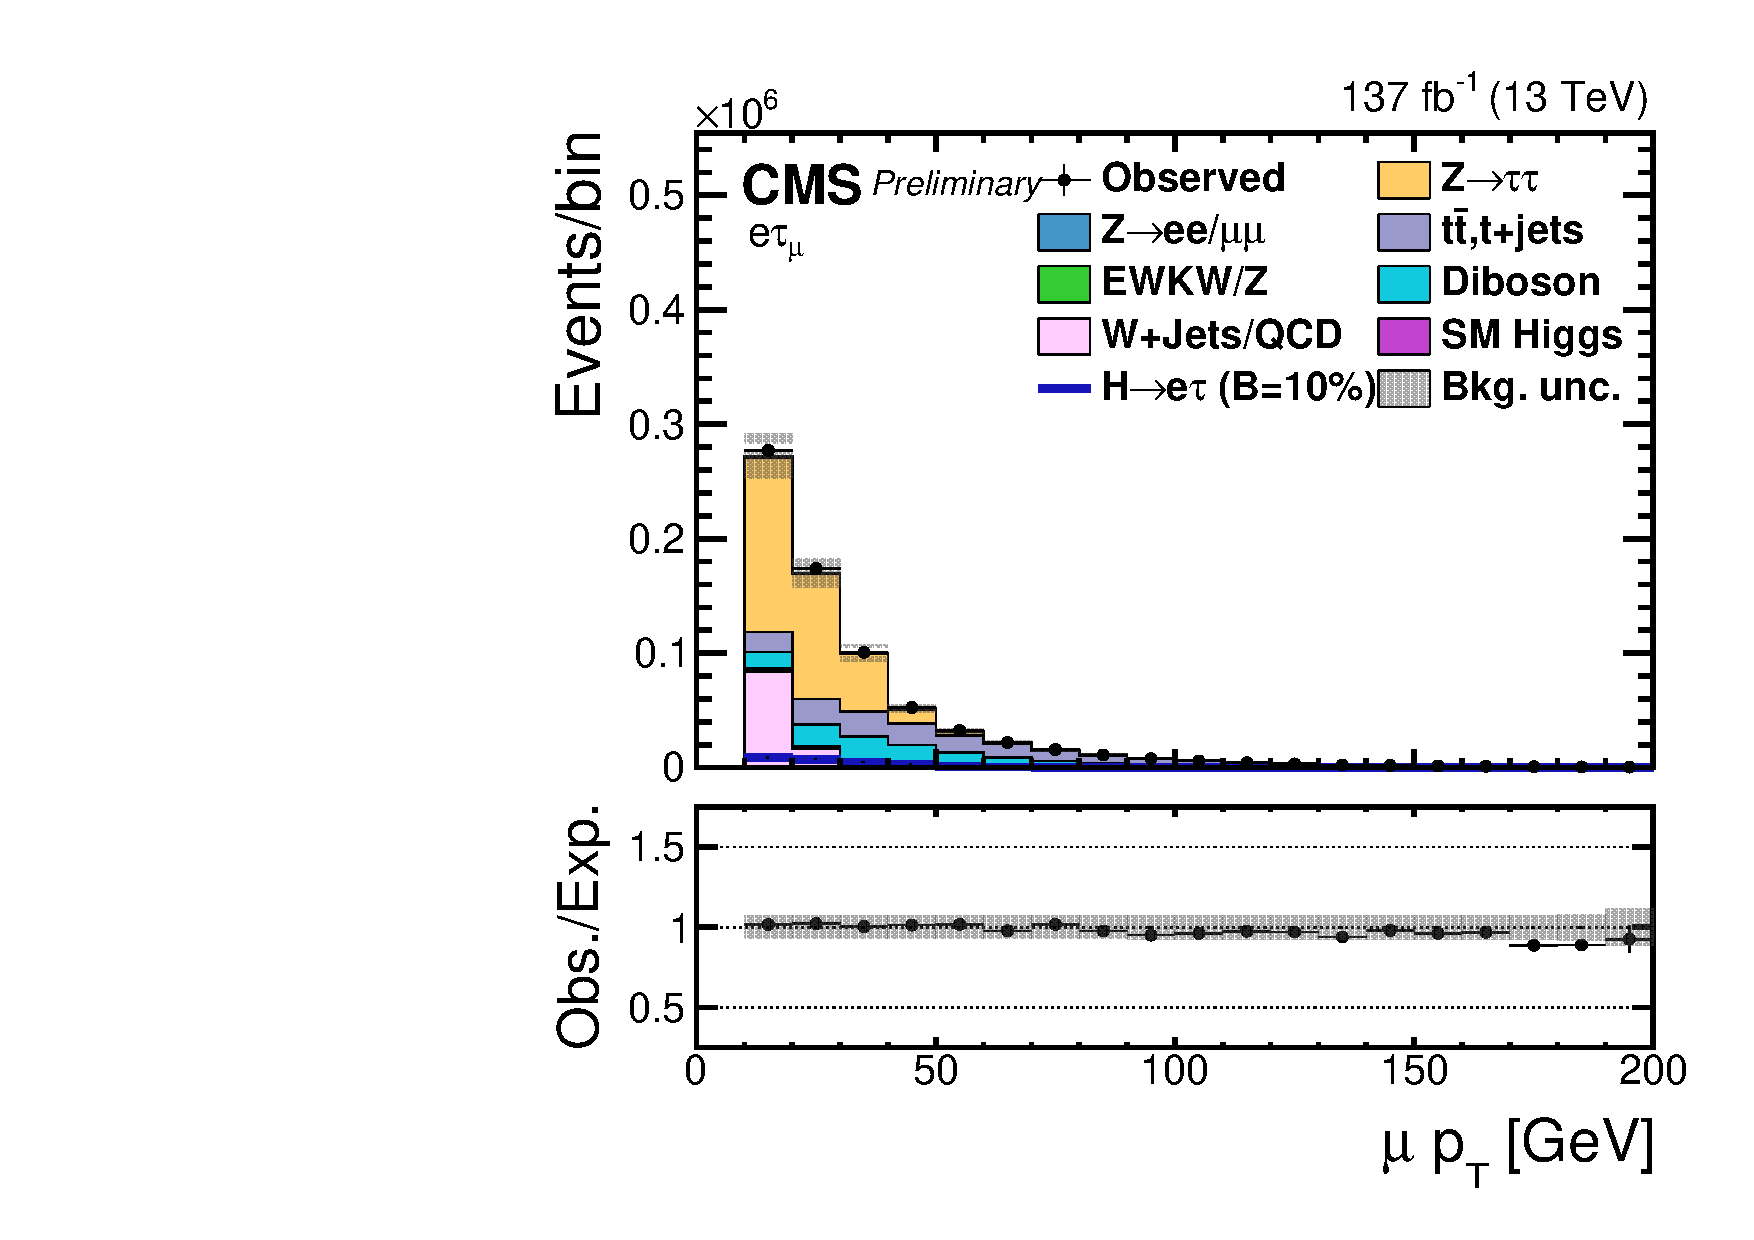
\includegraphics[width=0.36\textwidth]{plots/chapter6/emu/mPt.pdf}
  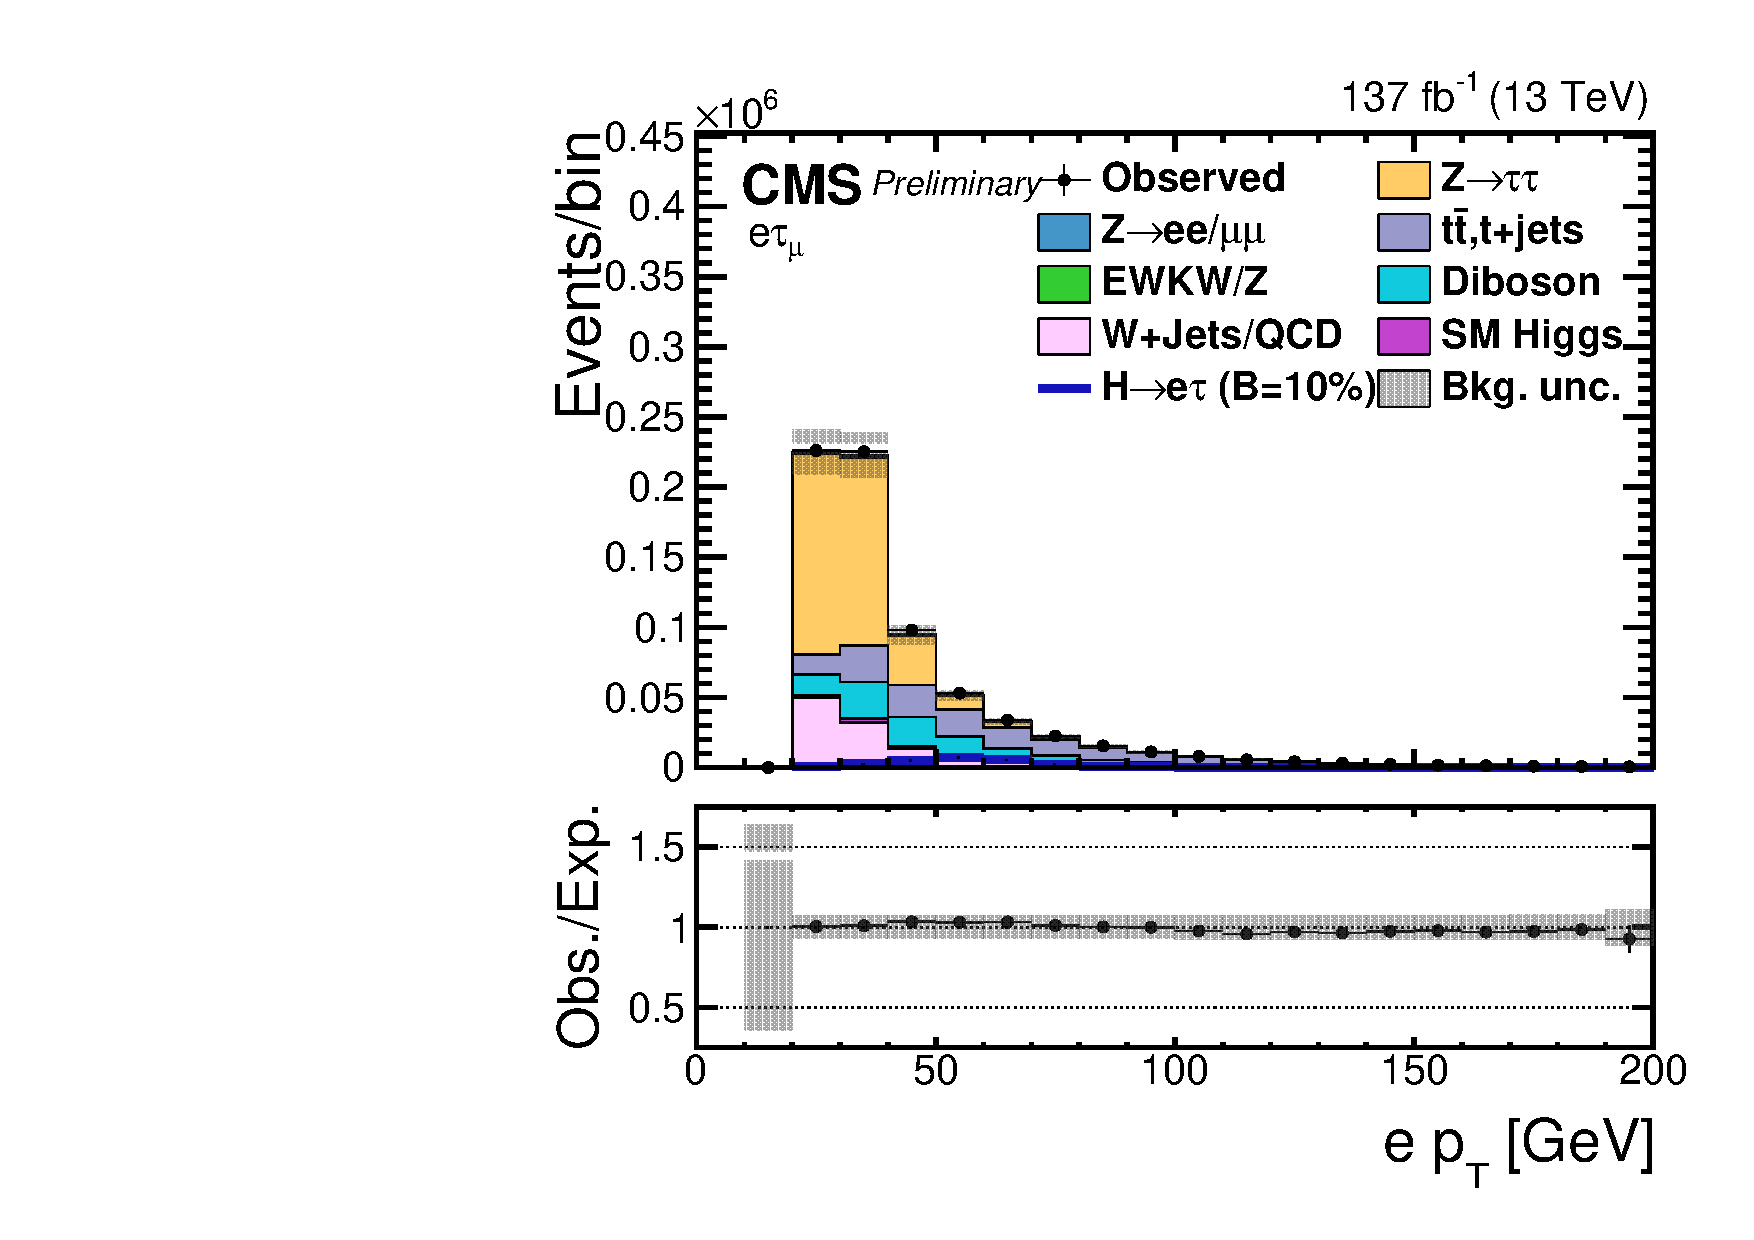
\includegraphics[width=0.36\textwidth]{plots/chapter6/emu/ePt.pdf}\\
  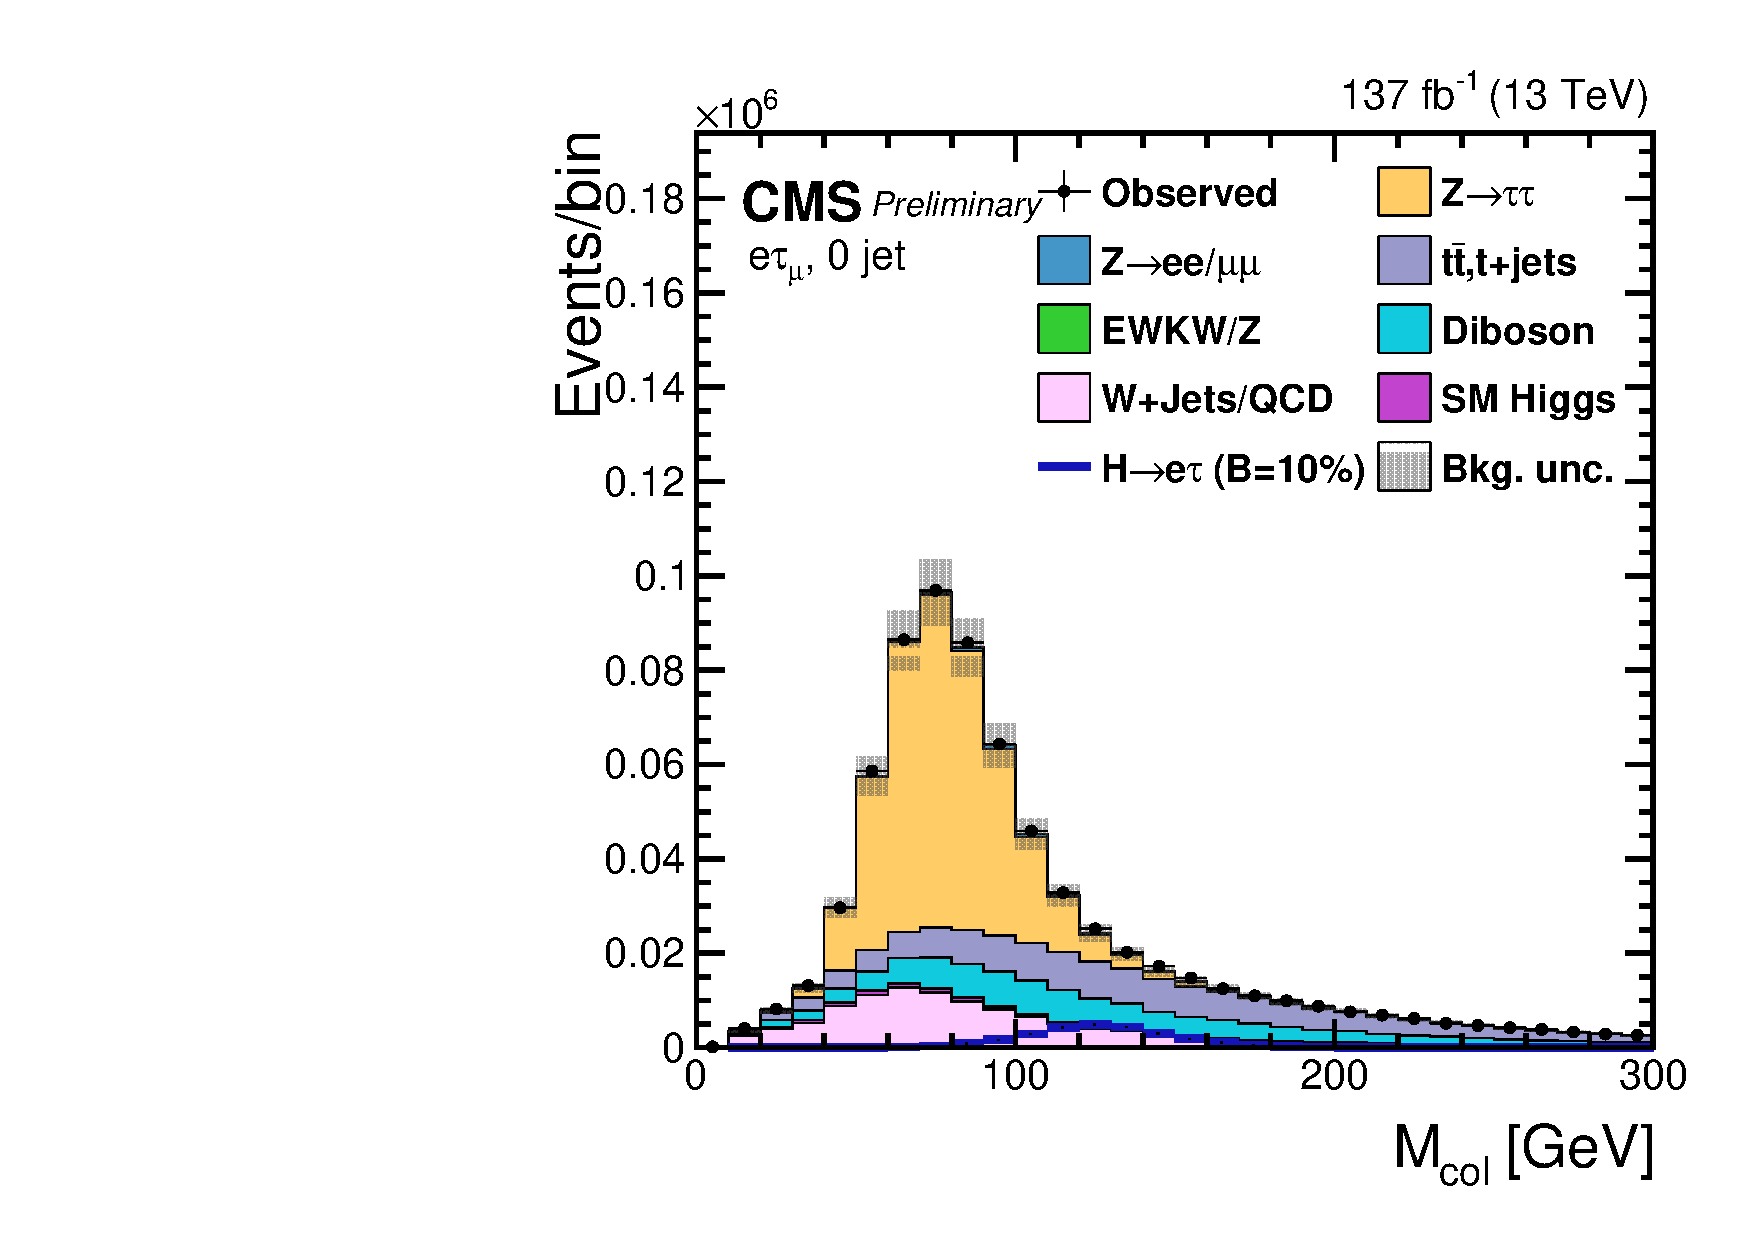
\includegraphics[width=0.36\textwidth]{plots/chapter6/emu/e_m_CollMass.pdf}
  \includegraphics[width=0.36\textwidth]{plots/chapter6/emu/e_m_Mass.pdf}\\
  \includegraphics[width=0.36\textwidth]{plots/chapter6/emu/dPhiMuMET.pdf}
  \includegraphics[width=0.36\textwidth]{plots/chapter6/emu/dPhiEMET.pdf}\\
  \includegraphics[width=0.36\textwidth]{plots/chapter6/emu/dPhiEMu.pdf}
  \includegraphics[width=0.36\textwidth]{plots/chapter6/emu/MTMuMET.pdf}\\
  \caption{Distribution of the input variables to the BDT for the \Hemu process.}
  \label{fig:input_em}
\end{figure}

In the \mcol fit method, additional selection criteria require a stringent selection on electrons, $\pt > 30\GeV$ for $0-$jet category and $\pt > 26\GeV$ in rest of the categories. The \mt(\Pe, \ptvecmiss) is required to be greater than 60, 40, 15 and 15\GeV for $0-, 1-, 2-$jet GGF and VBF categories, respectively, while azimuthal separation between the muon and \ptvecmiss is required to be less than 0.7, 0.7, 0.5 and 0.3 for $0-, 1-, 2-$jet GGF and VBF categories, respectively. For the $0-$ and $1-$jet categories $\dphiem > 2.5$ and 1.0, respectively. The selections for both \Hehad and \Hemu channels in all categories are also summarized in Table ~\ref{tab:etau_evtselection}. The \mcol distributions of simulated signal, data, and backgrounds for each category in \Hemu channel, are shown in results chapter.

\begin{figure}[htbp]
  \centering
  \subfigure[]{\includegraphics[width=0.32\textwidth]{plots/chapter6/BDT/emu/2016.pdf}}
  \subfigure[]{\includegraphics[width=0.32\textwidth]{plots/chapter6/BDT/emu/2017.pdf}}
  \subfigure[]{\includegraphics[width=0.32\textwidth]{plots/chapter6/BDT/emu/2018.pdf}}
  \caption{Overtraining check as performed in TMVA for the trained BDT in \Hemu channel for 2016 (a), 2017 (b), and 2018 (c).}
  \label{fig:etaumu_bdttrain}
\end{figure}
